%% This is file `elsarticle-template-1a-num.tex',
%%
%% Copyright 2009 Elsevier Ltd
%%
%% This file is part of the 'Elsarticle Bundle'.
%% ---------------------------------------------
%%
%% It may be distributed under the conditions of the LaTeX Project Public
%% License, either version 1.2 of this license or (at your option) any
%% later version.  The latest version of this license is in
%%    http://www.latex-project.org/lppl.txt
%% and version 1.2 or later is part of all distributions of LaTeX
%% version 1999/12/01 or later.
%%
%% The list of all files belonging to the 'Elsarticle Bundle' is
%% given in the file `manifest.txt'.
%%
%% Template article for Elsevier's document class `elsarticle'
%% with numbered style bibliographic references
%%
%% $Id: elsarticle-template-1a-num.tex 151 2009-10-08 05:18:25Z rishi $
%% $URL: http://lenova.river-valley.com/svn/elsbst/trunk/elsarticle-template-1a-num.tex $
%%
% \documentclass[preprint,12pt]{elsarticle}
%\documentclass[preprint,authoryear,12pt]{elsarticle}

%% Use the option review to obtain double line spacing
%% \documentclass[preprint,review,12pt]{elsarticle}

%% Use the options 1p,twocolumn; 3p; 3p,twocolumn; 5p; or 5p,twocolumn
%% for a journal layout:
%% \documentclass[final,1p,times]{elsarticle}
%%  \documentclass[final,1p,times,twocolumn]{elsarticle}
%% \documentclass[final,3p,times]{elsarticle}
%% \documentclass[final,3p,times,twocolumn]{elsarticle}
%% \documentclass[final,5p,times]{elsarticle}
\documentclass[final,authoryear,5p,times,twocolumn]{elsarticle}

%% if you use PostScript figures in your article
%% use the graphics package for simple commands
%% \usepackage{graphics}
%% or use the graphicx package for more complicated commands
%% \usepackage{graphicx}
%% or use the epsfig package if you prefer to use the old commands
%% \usepackage{epsfig}

%% The amssymb package provides various useful mathematical symbols
\usepackage{amssymb}
%% The amsthm package provides extended theorem environments
%% \usepackage{amsthm}

%% The lineno packages adds line numbers. Start line numbering with
%% \begin{linenumbers}, end it with \end{linenumbers}. Or switch it on
%% for the whole article with \linenumbers after \end{frontmatter}.
\usepackage{lineno}

%% natbib.sty is loaded by default. However, natbib options can be
%% provided with \biboptions{...} command. Following options are
%% valid:

%%   round  -  round parentheses are used (default)
%%   square -  square brackets are used   [option]
%%   curly  -  curly braces are used      {option}
%%   angle  -  angle brackets are used    <option>
%%   semicolon  -  multiple citations separated by semi-colon
%%   colon  - same as semicolon, an earlier confusion
%%   comma  -  separated by comma
%%   numbers-  selects numerical citations
%%   super  -  numerical citations as superscripts
%%   sort   -  sorts multiple citations according to order in ref. list
%%   sort&compress   -  like sort, but also compresses numerical citations
%%   compress - compresses without sorting
%%
%% \biboptions{comma,round}

% \biboptions{}

\usepackage{amsmath}
% \usepackage{breqn}
% \ExplSyntaxOn
% \cs_set_eq:NN \intexpr_eval:w \int_eval:w
% \cs_set_eq:NN \intexpr_eval_end: \int_eval_end:
% \ExplSyntaxOff


\usepackage{subfigure}
\usepackage{changepage}


\journal{Journal of Applied Geophysics}

\begin{document}

\begin{frontmatter}

%% Title, authors and addresses

%% use the tnoteref command within \title for footnotes;
%% use the tnotetext command for the associated footnote;
%% use the fnref command within \author or \address for footnotes;
%% use the fntext command for the associated footnote;
%% use the corref command within \author for corresponding author footnotes;
%% use the cortext command for the associated footnote;
%% use the ead command for the email address,
%% and the form \ead[url] for the home page:
%%
%% \title{Title\tnoteref{label1}}
%% \tnotetext[label1]{}
%% \author{Name\corref{cor1}\fnref{label2}}
%% \ead{email address}
%% \ead[url]{home page}
%% \fntext[label2]{}
%% \cortext[cor1]{}
%% \address{Address\fnref{label3}}
%% \fntext[label3]{}

\title{Data Quality Control Methodologies for Large, Non-Conventional DC Resistivity Datasets}

%% use optional labels to link authors explicitly to addresses:
%% \author[label1,label2]{<author name>}
%% \address[label1]{<address>}
%% \address[label2]{<address>}

\author{Michael A. Mitchell and Douglas W. Oldenburg}

\address{Geophysical Inversion Facility (GIF), \\
Department of Earth, Ocean and Atmospheric Sciences, \\
University of British Columbia, \\
2020-2207 Main Mall, \\
Vancouver, British Columbia \\
Canada, V6T 1Z4}

\begin{abstract}
With developments in instrumentation and computational resources, the collection of large, non-conventional DC resistivity datasets has become commonplace. While the increased data content of these large datasets can significantly improve the resolution of inverse models, these datasets also present challenges for standard data quality control (QC) methodologies. Standard QC methodologies for DC resistivity datasets typically rely on our ability to decompose the dataset into 2D lines and/or reciprocal measurements. Non-conventional electrode geometries and the cost of collecting a large number of reciprocal measurements can severely limit the applicability of standard DC resistivity QC methodologies.

To address these limitations, we developed a more generalized data QC methodology which utilizes statistical analysis and classification tools. The merit of this methodology is illustrated using a field dataset collected in an underground potash mine and several synthetic examples. Results from these applications show that the methodology has the ability to identify and characterize highly noise-contaminated data from a number of different sources. The flexibility of the 4-stage methodology allows it be tailored to accommodate data from any type of DC resistivity survey and the use of statistical analysis and classification tools decreases the subjectivity of the process. Although this study focuses on the applicability of this methodology for DC resistivity data, it is potentially applicable to a variety of geophysical surveys.  

\end{abstract}

\begin{keyword}
%% keywords here, in the form: keyword \sep keyword
DC resistivity (ERT/ERI) \sep  Data Quality Control \sep 3D Inversion \sep Data Clustering

%% MSC codes here, in the form: \MSC code \sep code
%% or \MSC[2008] code \sep code (2000 is the default)

\end{keyword}

\end{frontmatter}

%%
%% Start line numbering here if you want
%%
\linenumbers

%% main text

\section{Introduction}
\label{Introduction}

Despite the many advances in multi-channel instrumentation systems, survey design optimization, and inversion techniques, large DC resistivity datasets can still be difficult to work with due to limitations of standard data quality control (QC) methodologies. Identifying and dealing with highly noise-contaminated or inconsistent data is a vitally important part of the inversion process since it informs our choice of measurement uncertainties.  These uncertainties define the relative importance or weight of each measurement. Standard tools for data QC include 2D pseudo-section plots of apparent resistivity and repeat or reciprocal measurements.  

With 2D profiles, a pseudo-section of the apparent resistivities is typically plotted to highlight spurious or noise-contaminated data associated with a specific electrode \citep{Edwards1977,Deceuster2013}. Since the apparent resistivity is expected to vary smoothly in most circumstances, spurious data can be identified by small, anomalous regions of high or low apparent resistivity \citep{Loke2000}. Similarly, conventional 3D surveys, which consist of a regular grid of electrodes, are typically decomposed into 2D profiles so that pseudo-sections can be easily plotted \citep{Auken2006}. However, when working with large non-conventional 3D datasets, plotting a map or pseudo-section of the data is not straightforward or meaningful. Data with very different electrode geometries can plot in similar locations making it difficult to identify patterns associated with inconsistent or noisy data. 

Repeat and reciprocal measurements have been shown to be a useful tool for assessing the noise levels of DC resistivity datasets by several previous studies including \cite{LaBrecque1996}, \cite{Slater2000}, \cite{Zhou2003}, \cite{LaBrecque2008} and \cite{Wilkinson2012}. Repeat measurements are made anytime that the same transmitter (TX) and receiver (RX) locations are reoccupied, while reciprocal measurements are made when the TX and RX locations are interchanged. A formal proof of the reciprocity theorem for DC resistivity, assuming an arbitrary conductivity model, is given by \cite{Parasnis1988}. Reciprocal measurements provide a more reliable estimate of measurement noise levels since they account for some systematic error sources which can go undetected by repeat measurements \citep{LaBrecque1996}.  

While reciprocal measurements are certainly a valuable tool for assessing the noise level of DC resistivity datasets and identifying noise-contaminated measurements a full set of reciprocal measurements is not always collected. In large distributed array systems, such as Quantec's Titan 24 system, a dense grid of RXs is laid out and the TX is moved through the grid between the RXs. Since the RX locations are never occupied by the TX, no reciprocal measurements are collected with this setup. In other scenarios, limited budgets and a desire to maximize the data content of the survey prohibits the collection of a large number of reciprocal measurements. If a large non-conventional 3D dataset lacks sufficient reciprocal measurements, other methods must be employed to QC highly noise-contaminated data.

\subsection{Inversion Background}

After initial efforts to quality control the data and remove clear outliers, the data are input into an inversion algorithm to find a geologically reasonable conductivity model which acceptably reproduces the data. Since the inverse problem is typically very under-determined, (i.e. there are far more model cells than data), we pose it in a regularized optimization context as the minimization of a global objective function ($\Phi$). The inverse problem is solved by finding an estimate of the true model ($\widehat{m}$), which minimizes the model objective function ($\Phi_m$), while driving the data misfit ($\Phi_d$) to its target level ($\Phi_{d}^*$). This minimization problem can be formalized in the following manner.
\begin{eqnarray}
\label{eq:globphi}
\min \Phi = \Phi_d+\beta\Phi_m \\
\mbox{s. t. } \Phi_{d} \leq \Phi_{d}^* \nonumber
\end{eqnarray}
where $\beta$ is a regularization parameter that controls the relative importance of the model objective function, which controls the complexity and smoothness of the model, and the data misfit. To obtain a meaningful solution to the inverse problem we need to choose a metric by which to measure the data misfit, assign reasonable uncertainties to each measurement, and define a target misfit to quantify an acceptable data fit \citep{Oldenburg2005}.

Data misfit provides a quantitative measure of the difference between the observed data ($d^{obs}$) and the predicted data ($d^{pred}$) derived through numerical modelling. The data are normalized potentials or resistance values which are computed by dividing the measured potential differences ($V_{MN}$) by their injection currents ($I$). An $L_p$ norm is typically used for this metric with the $L_2$ being the most commonly used and the $L_1$ norm sometimes employed to better handle outliers. Here we use a standard $L_2$ formulation for the data misfit ($\Phi_d$).
\begin{equation}
\Phi_d = \sum^{n}_{i=0}\left(\frac{d^{obs}_i-d^{pred}_i}{\xi_i}\right)^2 = \left\|\mathbf{W}_{d}\left(\mathbf{d}^{obs}-\mathbf{d}^{pred}\right)\right\|_2^2
\end{equation}
where $\xi$ are the standard deviations of the data which quantify measurement uncertainty. The data weighting matrix $\mathbf{W}_{d}$ is a diagonal matrix with $1/\xi$ on the main diagonal. Since these standard deviations are typically unknown, we must estimate these uncertainties, which account for discrepancies between the observed and predicted data. These uncertainties are often referred to as the noise model.

Developing a accurate noise model is challenging since many factors contribute to measurement uncertainty and each has different underlying statistical distributions. To capture the cumulative effect of the various factors in a single distribution, we assume that the noise is uncorrelated and Guassian. Under these conditions, the target misfit is given by the expected value, which equals the number of data, provided uncertainties have been assigned reasonably. While these assumptions are almost certainly incorrect, they have served researchers well. As per common practice the uncertainties are assigned as a percentage of each measurement plus a floor value, which is often dependent on the magnitude of survey measurements and the instrument precision.

To control the complexity of the recovered model, the following formulation for the model objective function ($\Phi_{m}$) is used.
\begin{equation}
\label{eq:modobjdiscr}
\Phi_m = \left\|\mathbf{W}_s(\mathbf{m}-\mathbf{m}_o)\right\|_2^2 + \sum^{3}_{i=1}\left\|\mathbf{W}_i\mathbf{m}\right\|_2^2
\end{equation} 

Where the first term controls the ``smallness'' of the model (i.e. how close the current model ($\mathbf{m}$) is to the reference model ($\mathbf{m}_o$)) and the summation contains directional derivative terms which control the smoothness of the model in each direction. $\mathbf{W}_s$ is a diagonal matrix containing cell weights while the three components of $\mathbf{W}_i$ ($\mathbf{W}_x$, $\mathbf{W}_y$, and $\mathbf{W}_z$) combine finite difference operators and face weight vectors in each direction. 

The optimization problem is solved iteratively using a Gauss-Newton based approach, where at each $\beta$ iteration the model update is estimated using an incomplete preconditioned conjugate gradient solver. The initial $\beta$ is chosen to be sufficiently large so that the $\Phi_m$ dominates the objective function \citep{Haber2004}.  $\beta$ is then iteratively cooled with each iteration, placing more emphasis on reducing $\Phi_d$ by allowing more structure to be incorporated into the model.

For additional information on geophysical inversion we refer the reader to the following books: \cite{Menke1989}, \cite{Parker1994}, \cite{Aster2012}, and \cite{Haber2014}. \cite{Oldenburg2005} provide a general overview of geophysical inversion in their tutorial while \cite{Li1994}, \cite{LaBrecque1996}, \cite{Loke1996}, \cite{Ramirez1996}, and \cite{Loke2013} are a few of the many papers which specifically discuss the inversion of DC resistivity data.

After inverting, data misfit plots are used to examine how well the recovered model fits the data. A global misfit ($\Phi_{d}$) close to the target misfit indicates that there is good overall agreement between the observed and predicted data. Looking at the distribution of individual data misfits can help identify clear outliers and provides an estimate of how many data have individual data misfits greater than the target misfit of 1. If the recovered model does a poor job of fitting the observed data then further data quality control (QC) analysis is required.

\subsection{A New data QC Methodology}

The limitations of standard data QC tools prompted us to develop a new methodology which combines a search for correlations between high misfit data and various survey parameters with statistical analysis and classification tools to identify noise sources and deal with highly noise-contaminated and inconsistent data. Graphically this search for correlations can be done using a series of survey parameter cross-plots. However, this type of manual multivariate analysis is difficult since there are many parameter spaces to explore. Boxplots, SVD analysis, and $k$-Means clustering \citep{MacQueen1967} are used to semi-automate this procedure and reduce the subjectivity of the process. 

The data quality control methodology presented, is potentially applicable to a variety of field surveys. Here we test it in an underground environment with DC resistivity data. We find that a combination of a few poor electrodes and current leakage problems within the cables, that connect electrodes, have conspired to generate a highly noise-contaminated dataset. Despite the highly contaminated nature of the dataset, we are able to use the outlined data QC methodology to identify a subset of reliable data for inversion and obtain an interpretable inversion model.  

In this paper, we open with a description of the case history, which provided the impetus for this research, and then present the 4-stage data QC methodology in the context of the case history. The final results of the field data inversion and the results of several synthetic problems are shown to illustrate the utility of the methodology. We conclude with a discussion of the results and the performance of the data QC methodology. 
 
\section{Motivating Case Study}
\label{CaseStudy}

Engineers at the Mosaic K2 potash mine outside of Esterhazy, Saskatchewan have been combating water inflow problems for over a decade with limited success. In an effort to learn more about their problem a large non-conventional DC resistivity dataset was collected. Using this data, we aim to accurately image the source of the water inflow and map the conduits through which the water enters the mine.

The K2 mine has workings approximately 1 km beneath the surface, in the upper layers of the Middle Devonian (393-382 mya) Prairie Evaporite. Although several aquifers in the lower Dawson Bay Formation overlie the Prairie Evaporite, a roughly 20 m thick layer of evaporites and a dolomitic shale layer, known as the Second Red Bed, provide an impermeable membrane which keeps water from the permeable aquifers out of the mine. When the integrity of the Second Red Bed and the overlaying evaporite are weakened by naturally occurring voids and inhomogeneities or mining induced fracturing related to subsidence and ``creeping,'' water inflow problems often result. \cite{Gendzwill1992} and \cite{Chouteau1997} present a more detailed discussion of the types of problems encountered in potash mining and review many of the associated geophysical studies. Figure \ref{fig:Intro_ProblemCartoon} shows an overview of the mine environment and provides context regarding the geological setting.  

\begin{figure} [!ht]
    \begin{center}
       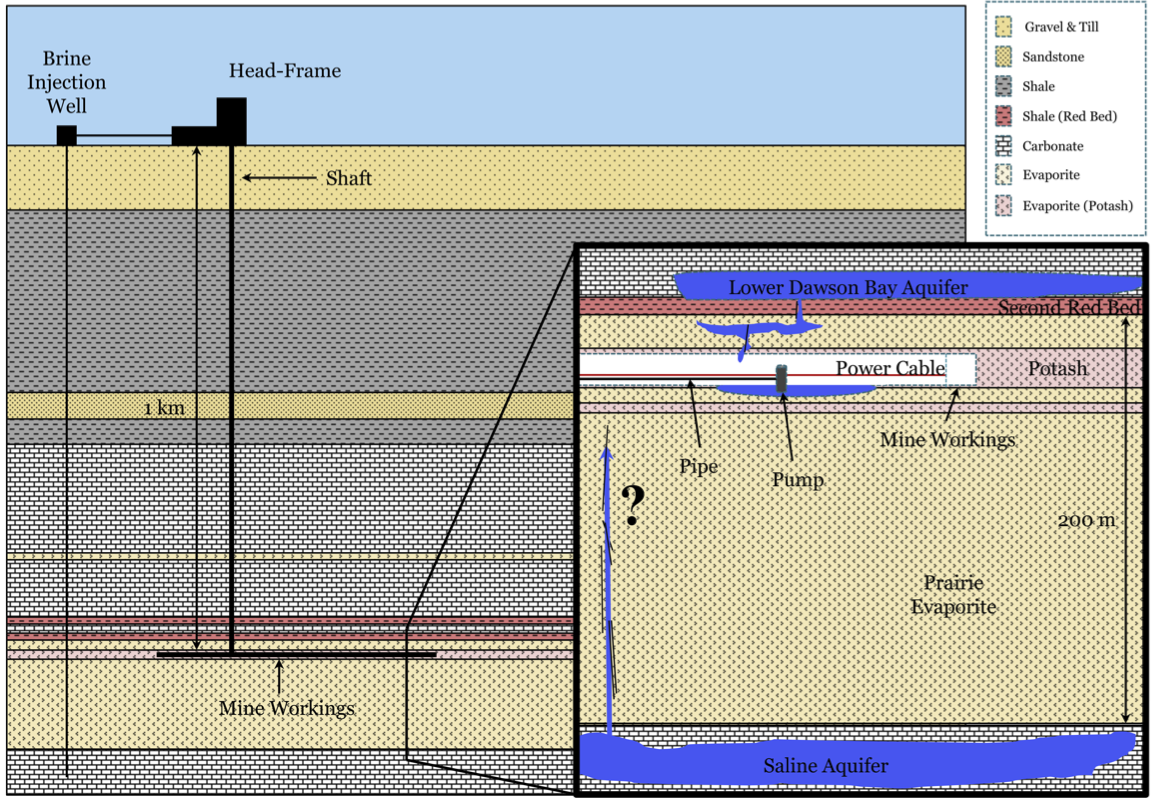
\includegraphics[trim=0cm 0cm 0cm 0cm, clip=true,width=1\linewidth]{./Figures/Fig1.pdf}
    \end{center}
\caption{A simple cartoon showing the basic overview of the K2 mine including its geological setting and mine infrastructure.} 
\label{fig:Intro_ProblemCartoon}
\end{figure} 

Like many other potash mines, the Mosaic K2 mine is currently having water inflow problems, which are largely due to mining induced fractures. To prevent flooding, an estimated 38,000L of brine per minute are being pumped out of the K2 mine. The brine is pumped to the surface and then injected back into a deeper aquifer. Recent developments have led mine officials to worry about the prospect of the brine injection over pressurizing the deeper aquifer. Under these circumstances water could be entering the mine both from above and below. These two threatening water sources are illustrated in Figure \ref{fig:Intro_ProblemCartoon}.       

Electrical and possibly electromagnetic (EM) methods offer the best chances of imaging the wet zones as a result of the large contrast in conductivity between the wet salt or briny water (0.1 - 20 S/m) and dry salt ($2.5 \times 10^{-5}$ - 0.01 S/m) \citep{Duckworth1992, Chouteau1997}. Identifying the location and geometry of these water bearing regions is vitally important to mining operations to avoid flooding. Accurate conductivity models of the region surrounding the mine workings can help the engineers identify and seal off current water inflow sources and hopefully avoid hitting water bearing zones in the future. 

\subsection{DC Resistivity Data and Instrumentation}
\label{CaseStudy:Data_Instrumentation}
The data used in this study were collected using a non-conventional 3D dipole-dipole array, which was designed and collected by Golder Associates. The full survey uses 120 stainless steel electrodes which are combined in a variety of combinations to form a survey comprised of 2,351 current electrode pairs (transmitters, TXs) and 95,194 associated potential electrode pairs (receivers, RXs). The measurements were collected using an IRIS Syscal Pro, which is a multi-channel switching system capable of simultaneously measuring 10 potential differences for a given TX (current dipole). Switching cables were 50 m long with electrode take-outs every 5 m. Six switching cables are linked with connecting boxes to connect electrodes 1-60 with the control box and another six switching cables are used to connect electrodes 61-120. We refer to these combined cables as Cable 1 and Cable 2 respectively. 

The geometry of the tunnels and the general layout of the electrodes are shown in Figure \ref{fig:DataQC_OctreeMesh_ElecGeom} while a typical TX is shown in Figure \ref{fig:DataQC_TypicalTx}. Within the mine, electrode placement is typically restricted to the mine workings (drifts-horizontal tunnels, raises-small vertical shafts, and smaller sub-drifts). Main drifts are typically 3-6 m wide and 3-4 m tall, most of the raises extend approximately 20 m vertically up to the Second Red Bed (Shale) above the Prairie Evaporite, and the sub-drifts are usually 2-3 m wide and 2-3 m tall. The electrodes are laid out along the interior tunnel walls as shown in Figure \ref{fig:DataQC_OctreeMesh_ElecGeom} with a spacing of 5 m to image the central region between the tunnels, where a water inflow source is suspected.

\begin{figure} [!ht]
    \begin{center}
    \subfigure[Discretized tunnel and electrode geometry]{%
       \label{fig:DataQC_OctreeMesh_ElecGeom}
       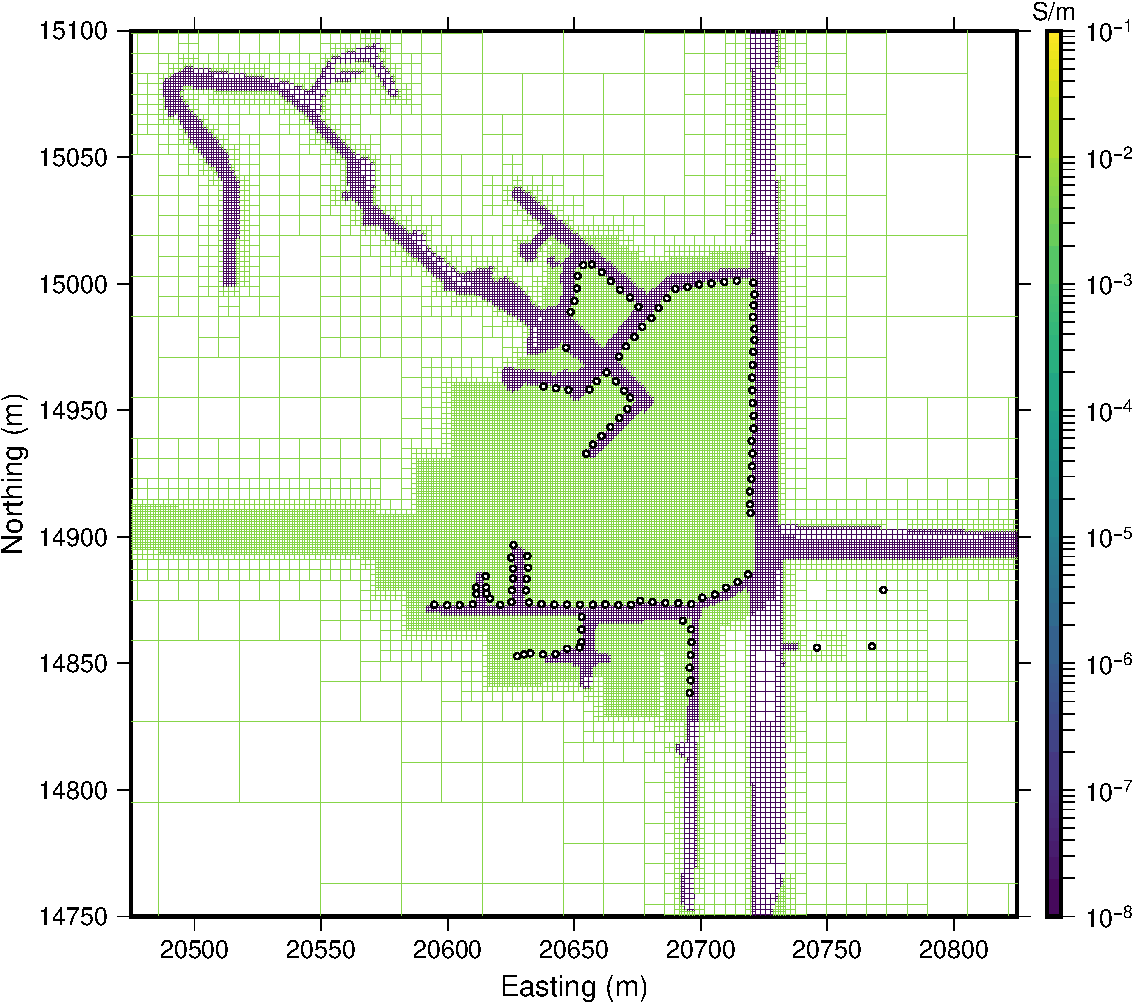
\includegraphics[trim=0cm 0cm 0cm 0cm, clip=true,width=0.95\linewidth]{./Figures/Fig2a.pdf}
       } \\%
    \subfigure[Typical TX with associated RXs]{%
       \label{fig:DataQC_TypicalTx}
       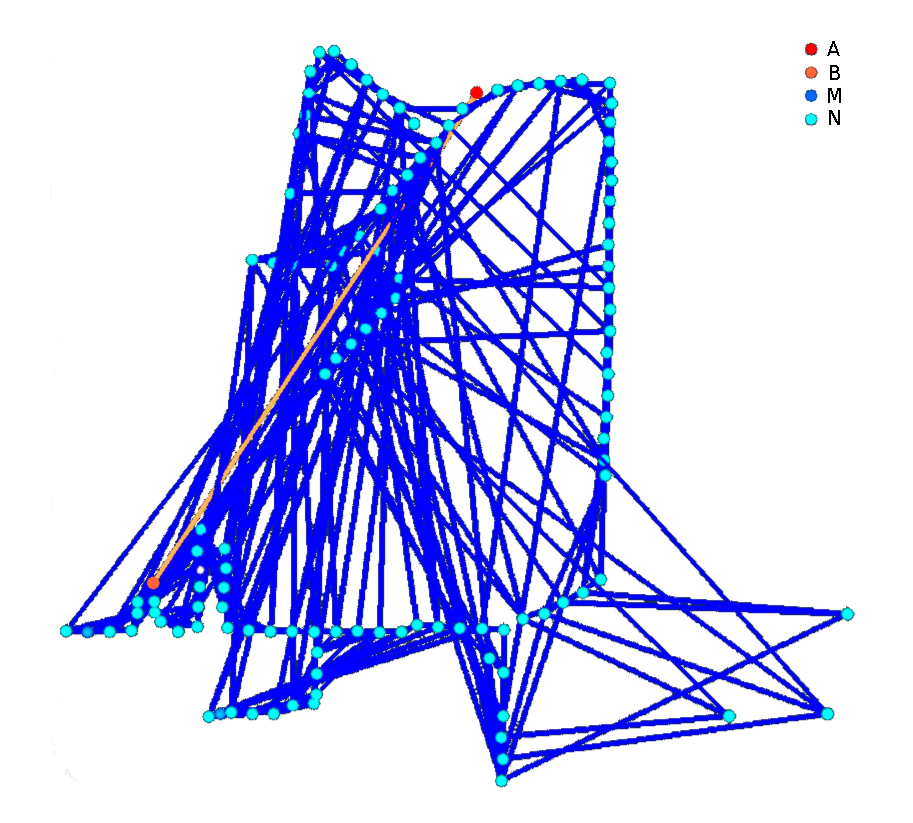
\includegraphics[trim=0cm 0cm 0cm 0cm, clip=true,width=0.75\linewidth]{./Figures/Fig2b.pdf}
       }
    \end{center}
\caption{Plot \ref{fig:DataQC_OctreeMesh_ElecGeom} shows the layout of the discretized tunnels (blue resistive cells) on the octree mesh and the location of all 120 electrodes (marked by white spheres) while plot \ref{fig:DataQC_TypicalTx} shows a typical TX (connected with the orange line) and its 349 associated RX electrode pairs (connected with blue lines). Electrodes 1-60 (connected with Cable 1) fall south of the gap in electrodes near the location (20720m, 14900m) while electrodes 61-120 (connected with Cable 2) are north of this gap.} 
\label{fig:DataQC_Layout}
\end{figure}

In the most basic sense DC resistivity measurements are made by injecting a constant current into the ground and measuring the associated potential differences set up by the currents. For a dipole-dipole experiment the current is injected between the A and B electrodes and one or more potential measurements are made between M and N electrode pairs. In this way each A-B electrode pair constitutes a TX and each M-N electrode pair a RX. To avoid problems with electrode polarization, the TX electrode locations are switched frequently to give charge build-ups near the current electrodes a chance to dissipate \citep{Dahlin2000}. Rapid reversals of the injection current orientation as part of a standard plus-minus-plus current injection cycle also help mitigate electrode polarization problems and cancel out spontaneous potential (SP) effects \citep{Telford1990, Dahlin2000}.

\section{Initial Inversions}
\label{Initial_Inv}
In preparation for the initial inversion we must first design a mesh. Since the tunnels are on average 3-4 m square in cross section and an electrode separation distance of 5 m was used, the problem was discretized onto an octree mesh with a minimum cell size of 1 m cubed (See Figure \ref{fig:DataQC_OctreeMesh_ElecGeom}). This insured that there were at least 3 cells between adjacent electrodes to reduce discretization errors around the current electrodes. The core region between the tunnels was also refined to the minimum cell size and 10 small cells were required adjacent to each electrode location. This insured that large discretization errors were not introduced by coarsening the mesh too rapidly near electrodes or regions of the model which might contain conductivity anomalies of interest. Mesh validation tests show that 95$\%$ of the forward modeled data from a 0.005 S/m full-space have discretization errors smaller than 2$\%$ when compared to the analytic solution. An octree mesh, in which the cell refinement is a function of the electrode locations and any structures in the reference conductivity model was used to greatly reduce the number of model cells from that of a standard tensor mesh. \cite{Haber2007} and \cite{Haber2012} provide a good discussion of the details associated with solving electromagnetic forward and inverse problems on octree meshes. 

Normalized potentials were computed by dividing the measured potential differences ($V_{MN}$) by their injection currents ($I$), and initial uncertainty estimates of $5\%$ plus a floor of 2 mV/A were assigned. If necessary, uncertainties can be modified during the data QC process to account for new insight into the distribution of noise.  
 
After testing several conductivities between 0.01 and 0.001 S/m a background conductivity of 0.005 S/m was selected for the reference and initial models. This background conductivity is consistent with literature values for the Prairie Evaporite \citep{Duckworth1992,Chouteau1997} and the observed apparent resistivities. The reference and initial models are uniform except for the air cells of the discretized tunnels which have a conductivity of $1 \times 10^{-8}$ S/m and are set as inactive cells in the inversion. All forward modeling and inversion results were obtained using the DCIP3D octree code developed by the UBC-GIF research group. For a more detailed description of the DCIP3D octree code please refer to the manual \citep{DCIP3D_Octree_Manual}.

\subsection{Initial Inversion Results}
\label{InitialInvResults}

Although the large scale conductivity structures in the recovered model seem geologically reasonable (See Figure \ref{fig:DataQC_FullInvResult}), the high normalized data misfit indicates that the model does not fit the observed data to within the tolerances specified by the assigned uncertainties (See Figure \ref{fig:DataQC_FullMisfitCurve}). Inspection of the individual misfits revealed that the high global data misfit was not due to a few outliers in the data, but was instead a more wide spread problem. Approximately 25-30$\%$ of the data fall within a band of high normalized misfits between 10-20 (See Figure \ref{fig:DataQC_FullMisfitHist}). Since the uncertainties were assigned assuming $5\%$ error plus a floor of 2 mV/A, a normalized data misfit of 10-20 indicates that many of the data require an assigned uncertainty of $50-100\%$ to reach target misfit. Misfits of this magnitude show that the inversion is doing a very poor job of fitting a large proportion of our data. Extensive data QC analysis is required to identify noise sources and deal with highly noise-contaminated data which can bias inversion results.  

\begin{figure} [!ht]
    \begin{center}
    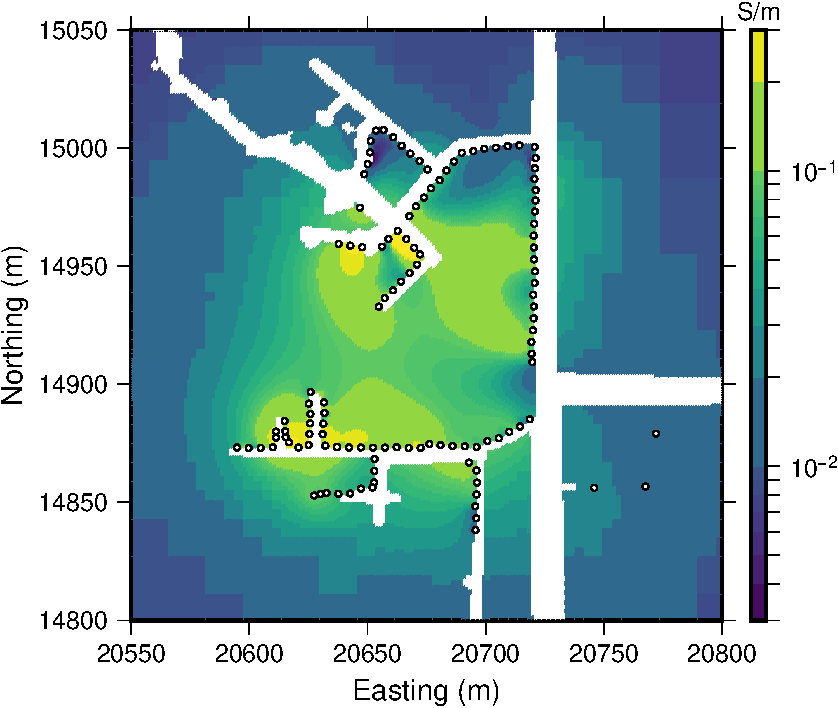
\includegraphics[trim=0cm 0cm 0cm 0cm, clip=true,width=0.95\linewidth]{./Figures/Fig3.pdf}
    \end{center}
\caption{A depth slice through the recovered conductivity model after the 10th inversion iteration. The electrode locations are marked by white dots. While the model seems geologically reasonable its validity is questioned due to the large data misfits shown in \ref{fig:DataQC_FullMisfit}.} 
\label{fig:DataQC_FullInvResult}
\end{figure}

\begin{figure} [!ht]
    \begin{center}
    \subfigure[]{%
       \label{fig:DataQC_FullMisfitCurve}
       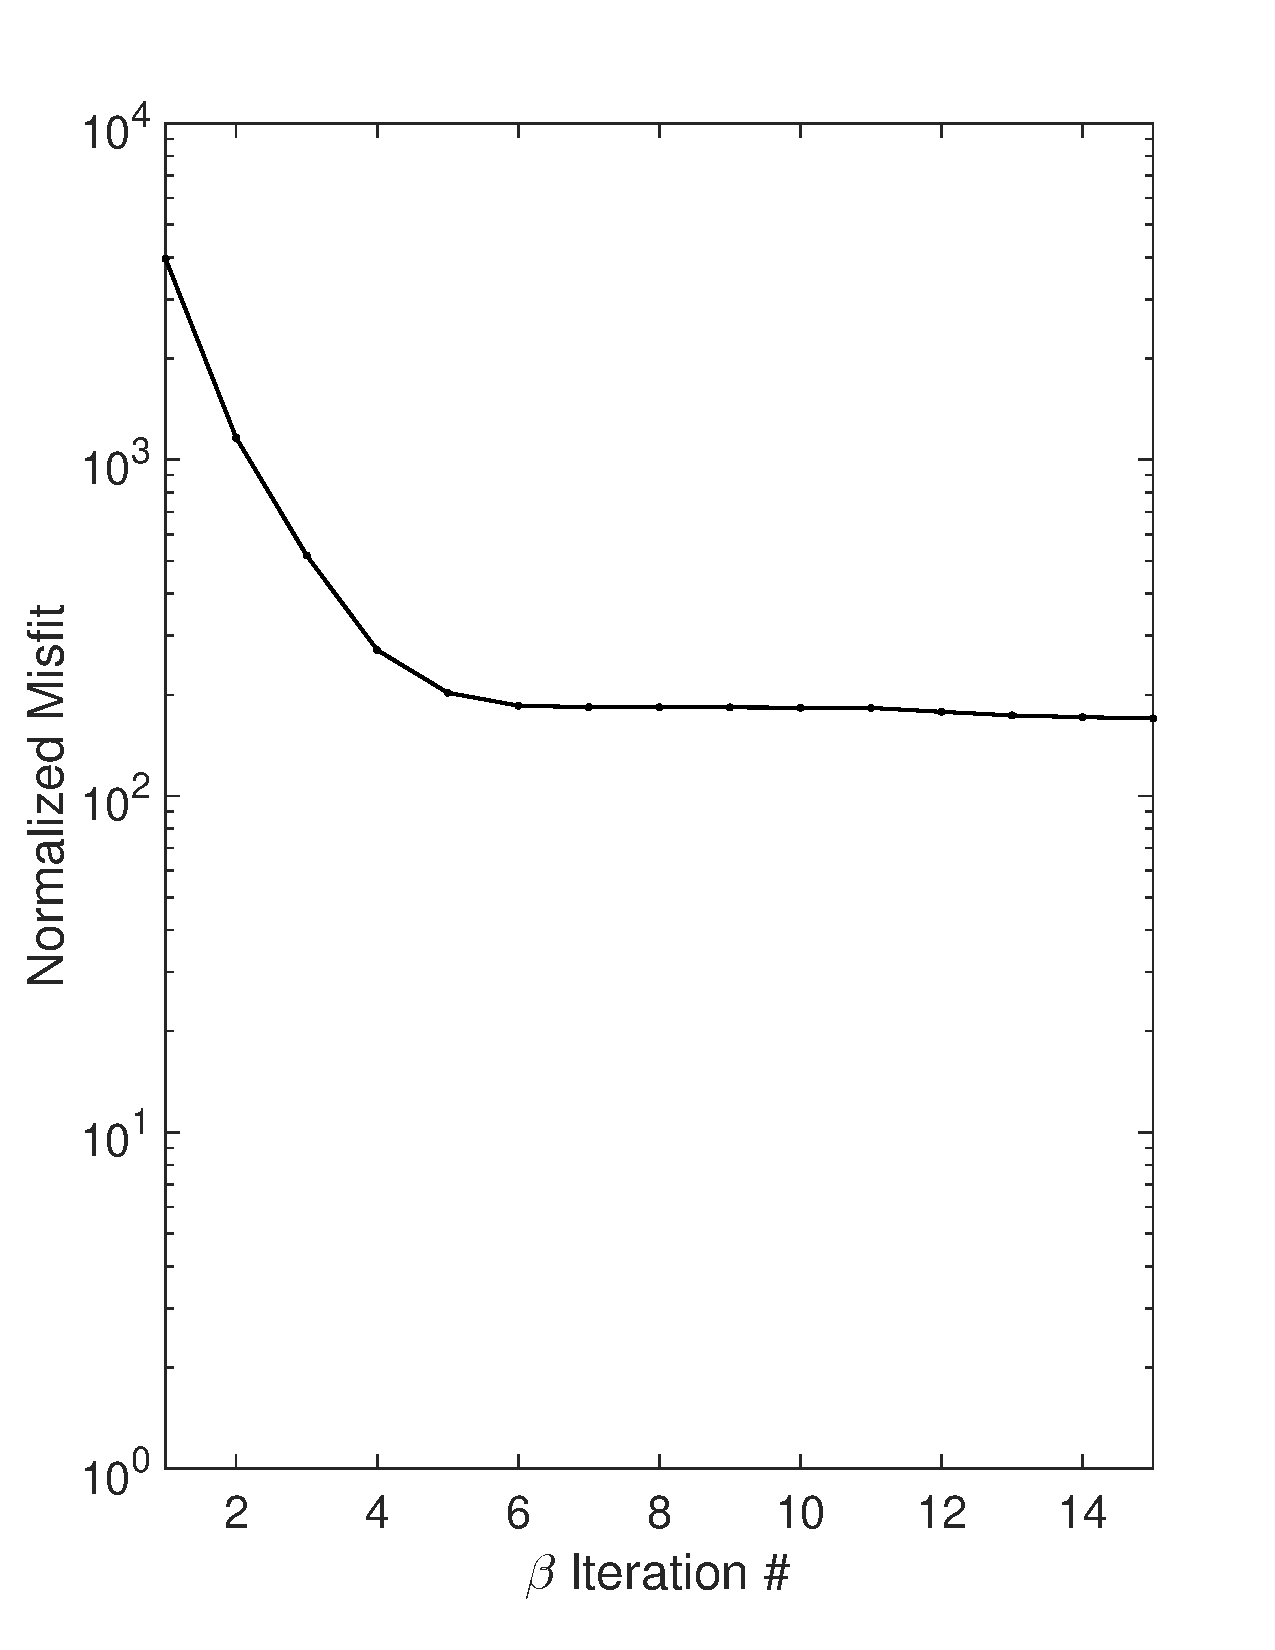
\includegraphics[trim=0.5cm 0.5cm 1.7cm 1cm, clip=true,width=0.475\linewidth]{./Figures/Fig4a.pdf}
       }
    \subfigure[]{%
       \label{fig:DataQC_FullMisfitHist}
       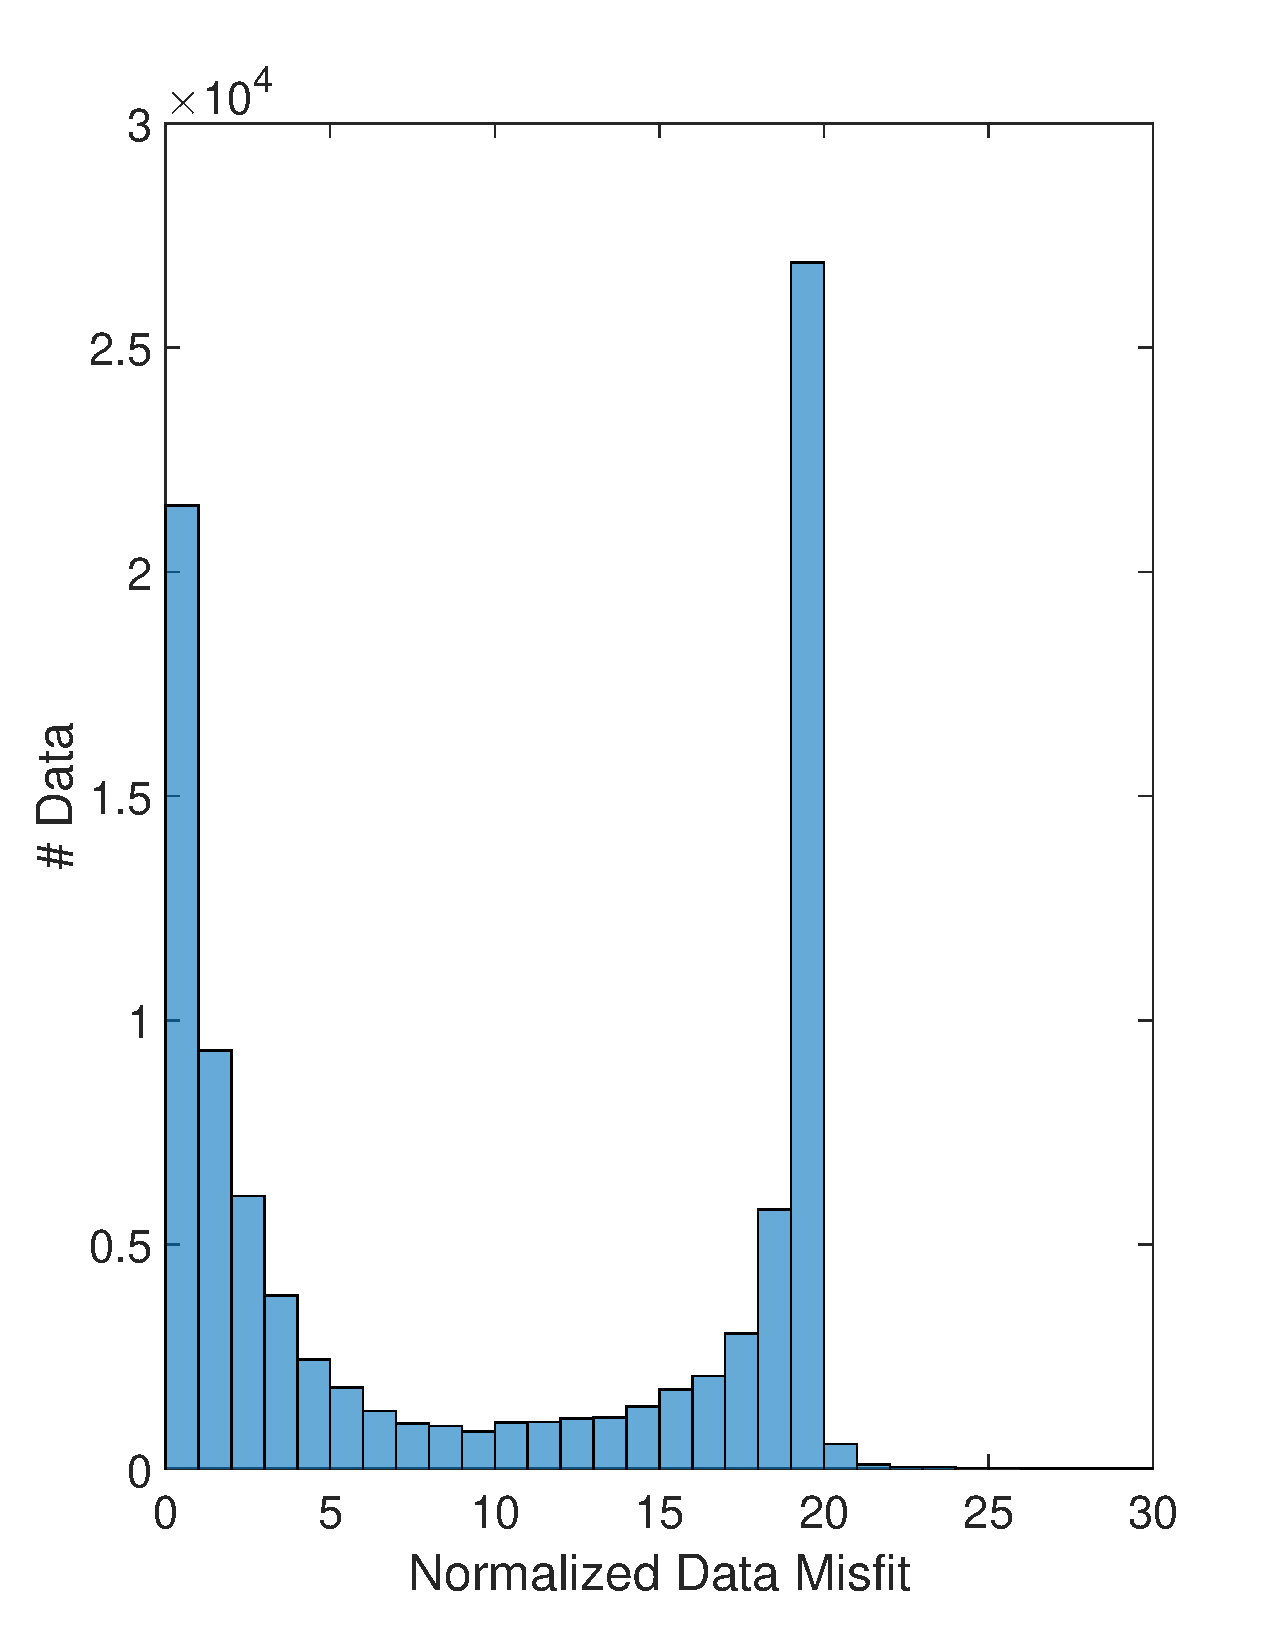
\includegraphics[trim=0.5cm 0.5cm 1.7cm 1cm, clip=true,width=0.475\linewidth]{./Figures/Fig4b.pdf}
       }
    \end{center}
\caption{\ref{fig:DataQC_FullMisfitCurve} shows the normalized misfit curve for the initial inversion. Near iteration 6 the global misfit plateaus 2 orders of magnitude above the target misfit of 1. A histogram showing the distribution of individual normalized data misfits is shown in panel \ref{fig:DataQC_FullMisfitHist}. The clear spike in the number of data with normalized misfits around 20 shows that a large proportion of the data is fit very poorly by the initial inversion.} 
\label{fig:DataQC_FullMisfit}
\end{figure}

\subsection{Dealing with High Data Misfits}
\label{Dealing_With_High_Misfits}
Since carefully sifting through data to weed out the highly noise-contaminated data can be very time consuming, short cuts are often taken and large quantities of data are thrown out. The danger in this is that in addition to discarding noise-contaminated data, important information about the perspective target may also be discarded. To avoid this pitfall, we need to focus more carefully on those factors which affect the data misfit. These factors can generally be lumped into the two following categories. 

\begin{enumerate}
   \item Data Quality Control
      \begin{itemize}
         \item Factors such as unaccounted for noise sources or unreasonably assigned uncertainties.
      \end{itemize}
   \item Inversion Limitations
      \begin{itemize}
         \item Any factors which control the model space and might cause the optimization algorithm to get trapped in a local minimum. 
      \end{itemize}
\end{enumerate}

For the sake of this study, we focus only on the data quality control based factors, but it is important to acknowledge that the inversion algorithm and our choice of the objective function also play important roles \citep{Farquharson1998,Oldenburg2005}. A detailed analysis of the field data was undertaken to form a reliable subset of data for inversion, develop a meaningful noise model, and identify the key sources of noise. To accomplish this we developed a set of tools and a methodology which can be used to standardize the data QC process and reduce its subjectivity.

\section{Data Quality Control}
\label{Data_Quality_Control}

The data QC methodology that we developed begins with a thorough analysis of the data to identify possible noise sources and then utilizes a k-means clustering algorithm to help distinguish and characterize heavily noise-contaminated data. The general 4-stage methodology proceeds as follows:

\begin{itemize}
    \item Stage I: Search for possible noise sources and select data subsets worthy of further analysis.
    \item Stage II: Use data clustering analysis to identify and deal with highly contaminated and inconsistent data. 
    \item Stage III: Recombine clusters from individual subsets and check for inter-cluster consistency.
    \item Stage IV: Recombine data subsets to form a single inversion ready dataset and check for inter-subset consistency.
\end{itemize}

The methodology presented here assumes that initial estimates for data uncertainty were assigned and that preliminary inversions have been run. If clear outliers were evident within the dataset after the first inversion they were removed. If a large percentage of the data have high normalized data misfits, which cannot reasonably be dealt with by adjustments to the noise model, it is likely that the dataset contains highly noise-contaminated or inconsistent data and requires further data QC analysis.

\subsection{Stage I: Search for Possible Noise Sources}
\label{Data_Quality_Control:StageI}
The goal of the first stage is to identify possible noise sources and select data subsets worthy of further analysis (See outline in Figure \ref{fig:DataQC_workflow_StageI}). This search for possible noise sources allows us to gain a better understanding of the dataset and characterize the general distribution of various survey parameters. If we can identify the characteristic signature of specific noise sources we can quantify the impact each has on the dataset. If the dataset is highly contaminated by a systematic noise source it may be possible to isolate the most highly contaminated data and focus further analysis on the more reliable data subsets. 

\begin{figure} [!ht]
\begin{center}
   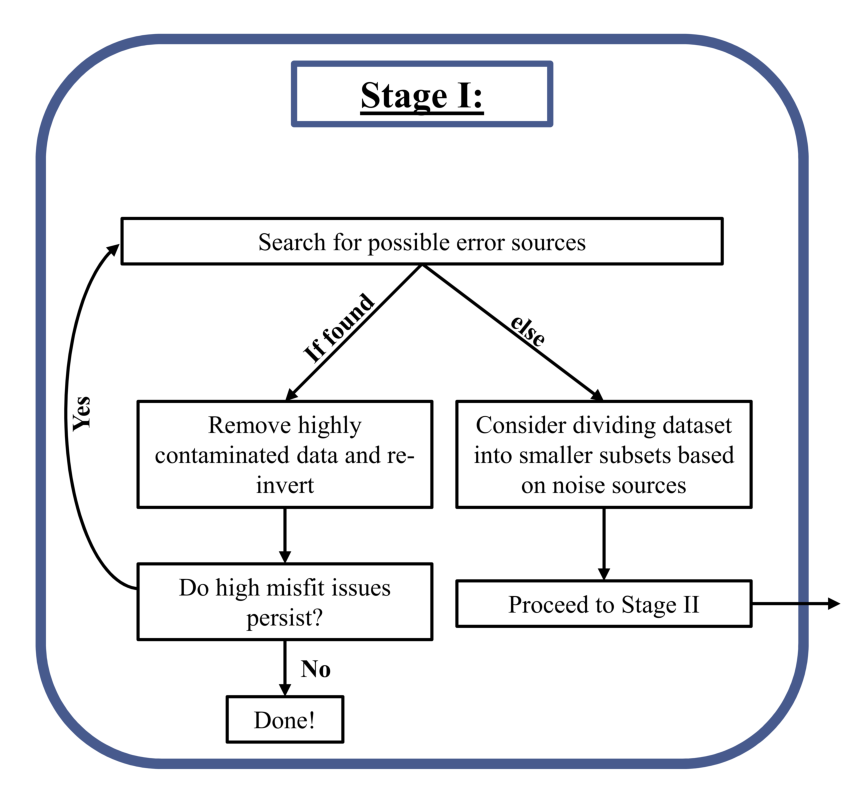
\includegraphics[trim=0cm 0cm 0cm 0cm, clip=true,width=0.75\linewidth]{./Figures/Fig5.pdf}     
\end{center}
\caption{Detailed workflow for Stage I.}
\label{fig:DataQC_workflow_StageI}
\end{figure}

We began by assessing modeling errors to insure that we had done an adequate job of discretizing the problem. This was done using mesh validation tests (Refer to the discussion of mesh design in Section \ref{Initial_Inv}) and an analysis of electrode location errors (See \ref{Appen:ElecLocErr}). Results showed no correlation between estimated modelling errors and high misfit data. 

Using cross-plots, repeat/reciprocal measurements, SVD analysis, and boxplots we checked for sources of correlated electrical noise. Some sources of correlated electrical noise might include: electrode polarization effects, high contact resistance of particular electrodes, electrical noise from infrastructure, current leakages within the multi-channel switch cables or connectors, and other instrument related malfunctions or calibration issues. Cross-plots of different survey parameters are often useful in identifying unusual correlations between certain survey parameters and high misfit data. Some useful parameters to plot include: potential differences between M and N RX electrodes ($V_{MN}$), potential differences across A and B TX electrodes ($V_{AB}$), injected currents ($I$), TX powers ($P_{AB}$), TX resistances ($R_{AB}$), apparent resistivities ($\rho_a$), electrode Ids, electrode separation distances, and timing variables. Determining which plots are the most meaningful for a particular dataset will require some experimentation.

For example, electrode polarization effects can often be characterized by calculating electrode rest times, which provide a measure of how long charge accumulations near the potential electrodes have been given to dissipate after having been used as a current electrode. To avoid electrode polarization errors, current electrodes need to be given a sufficiently long rest time for the polarization to decay before reoccupying them as potential electrodes \citep{Dahlin2000,Merriam2005,Wilkinson2012}. Any correlation between short electrode rest times and high data misfits should raise concerns about electrode polarization errors. Since no correlation of this type is observed in the field data electrode polarization effects are not believed to be a primary source of electrical noise.     

If available, repeat and reciprocal measurements should be analyzed to identify inconsistent measurements and provide a general assessment of noise levels. To quantify the consistency of each repeat/reciprocal pair the normalized data residual ($\tilde{r}$), which is the data difference divided by the sum of the uncertainties (See \ref{Appen:NDR}), was computed. Figure \ref{fig:DataQC_RepRecip_NDR_Hist} shows the distribution of normalized data residuals for all of the identified repeat/reciprocal pairs. While about half of the pairs have $\tilde{r} \leq 1$, many of the pairs have $\tilde{r}$ as large as 20. Here both repeat and reciprocal data show similar noise levels. These large $\tilde{r}$ indicate the presence of a pervasive noise source. A consistent repeat/reciprocal dataset is produced by removing the inconsistent data which have $\tilde{r} > 1$. 

\begin{figure} [!ht]
\begin{center}
    \subfigure[]{%
       \label{fig:DataQC_RepRecip_NDR_Hist_Num}
       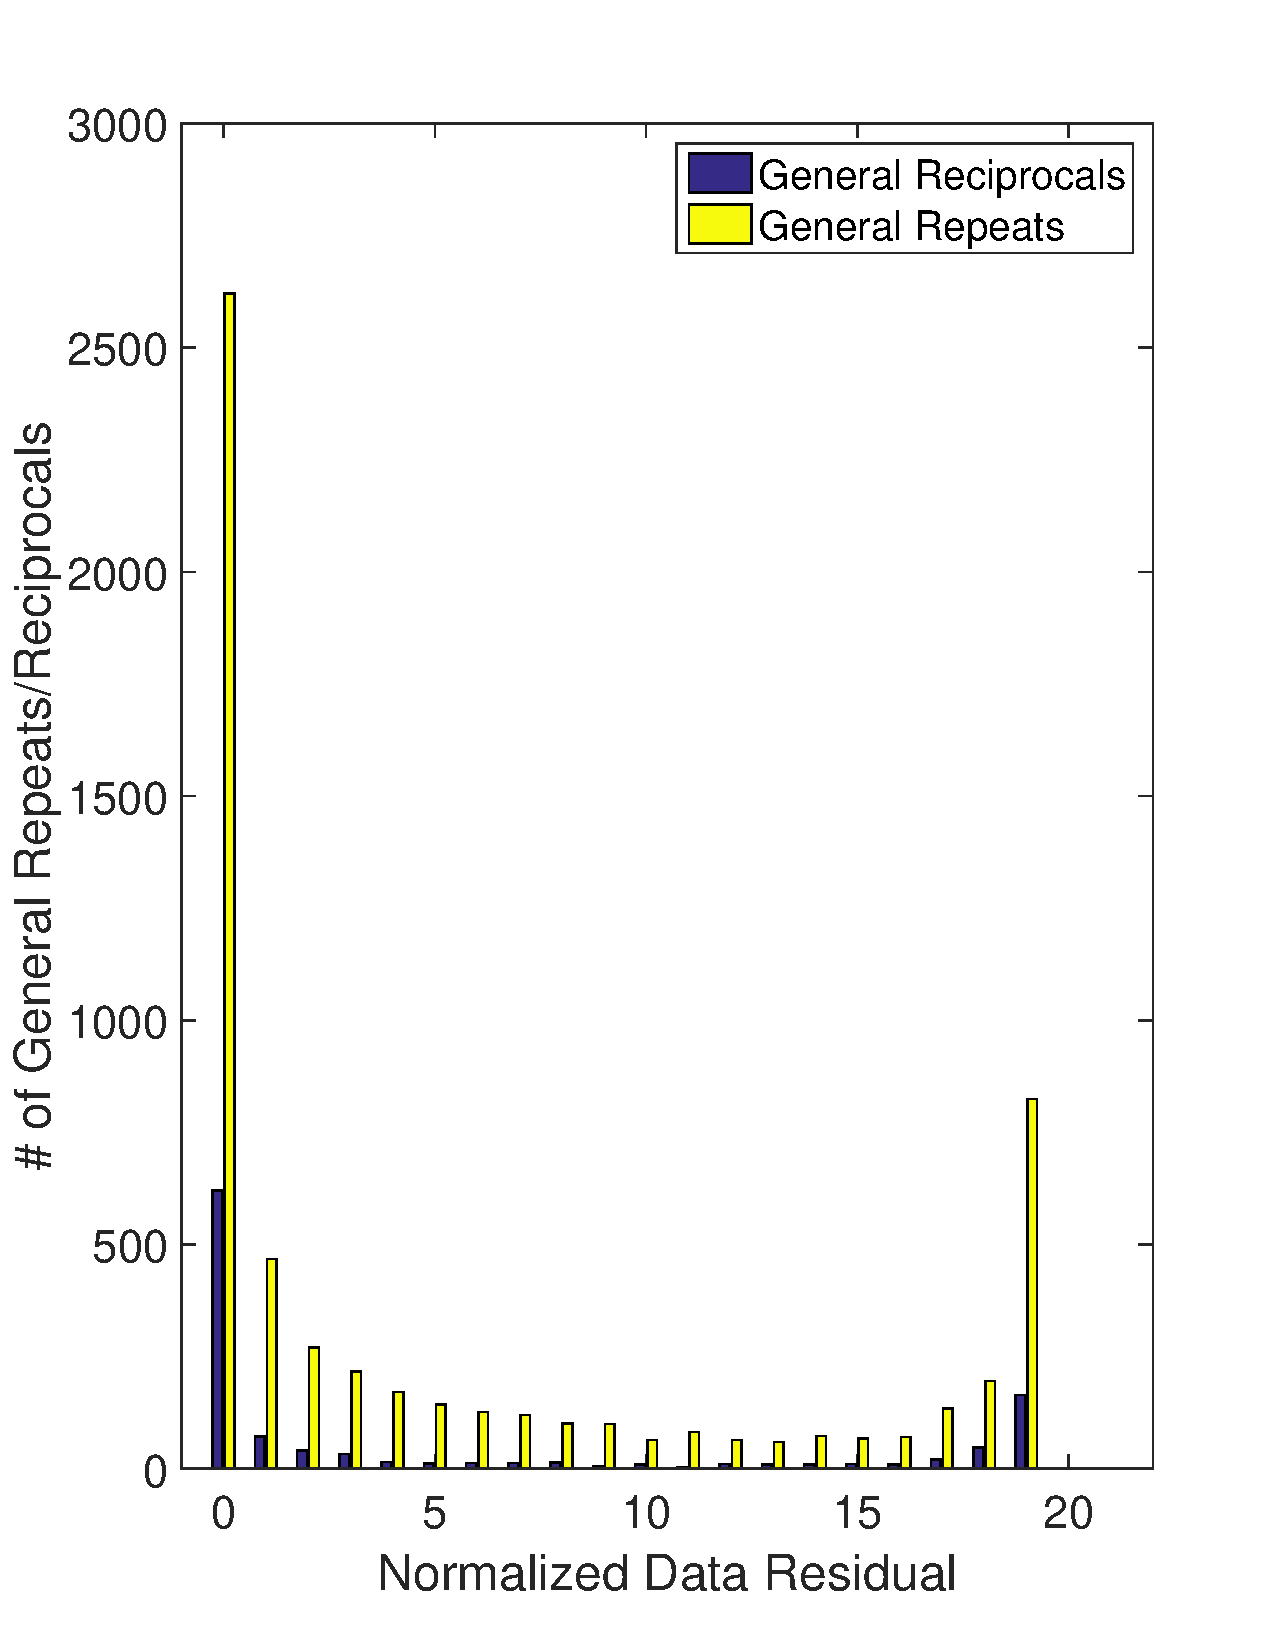
\includegraphics[trim=0.2cm 1cm 2cm 1.8cm, clip=true,width=0.475\linewidth]{./Figures/Fig6a.pdf}
       }%
    \subfigure[]{%
       \label{fig:DataQC_RepRecip_NDR_Hist_Perc}
       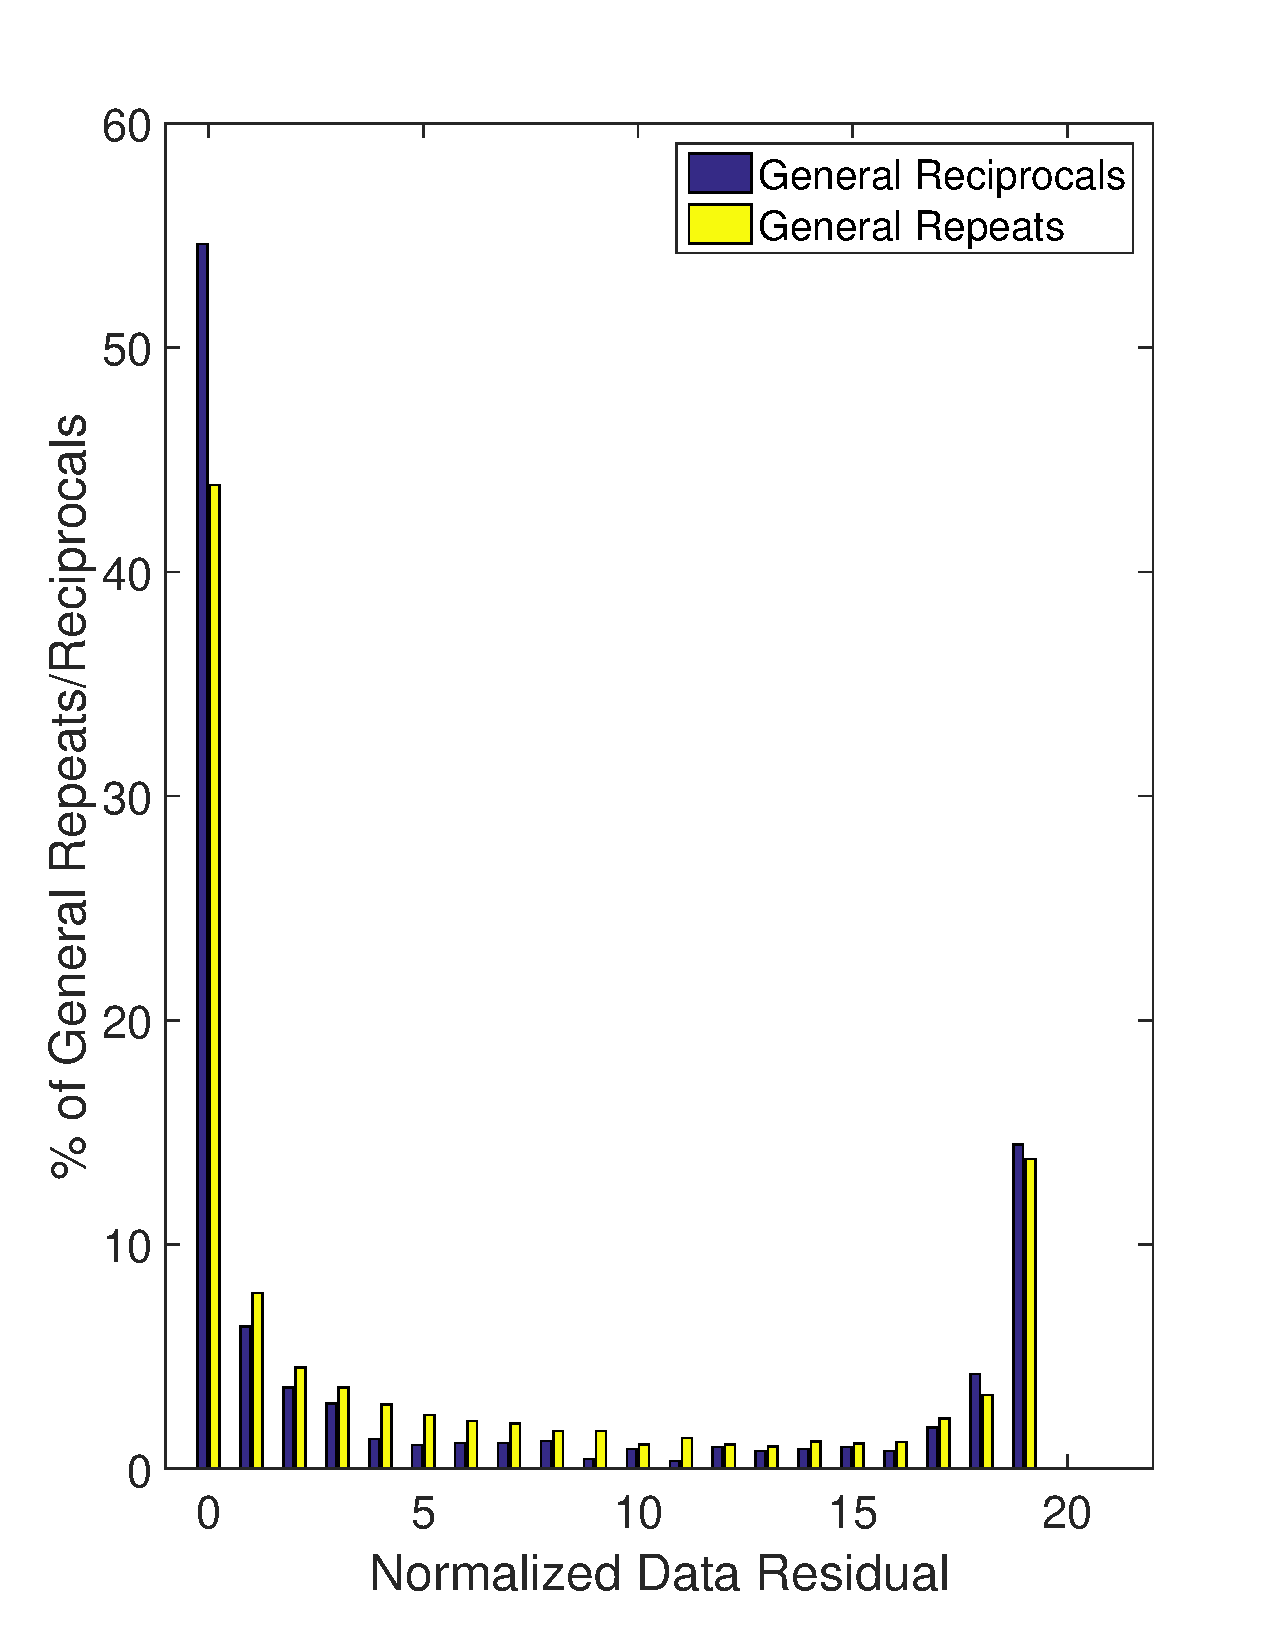
\includegraphics[trim=0.2cm 1cm 2cm 1.8cm, clip=true,width=0.475\linewidth]{./Figures/Fig6b.pdf}
       }
\end{center}
\caption{These histograms show the distribution of normalized data residuals ($\tilde{r}$) for all 7,109 repeat/reciprocal pairs identified in the dataset. \ref{fig:DataQC_RepRecip_NDR_Hist_Num} shows the total number of repeat/reciprocal pairs in each $\tilde{r}$ bin while \ref{fig:DataQC_RepRecip_NDR_Hist_Perc} shows them as a percentage of the total number of repeat or reciprocal measurement pairs. For both repeat and reciprocal data approximately $15 - 20\%$ of the pairs have $\tilde{r} > 15$.} 
\label{fig:DataQC_RepRecip_NDR_Hist}
\end{figure}     

After inverting the consistent repeat/reciprocal data subset high normalized data misfits persisted. This indicates that although the repeat/reciprocal pairs may be precise or self-consistent this does not insure that the pairs are accurate or consistent with one another. Careful analysis of the consistent repeat/reciprocal data showed general correlations between survey parameters such as high $V_{MN}$, low $I$, low $P_{AB}$, and high data misfits. However, selecting cutoffs for these parameters by which we can confidently separate the highly contaminated data from usable data is challenging and quite subjective.           

To identify the presence of electrical noise due to instrumentation problems or infrastructure more rigorous statistical analysis is often useful. Two valuable tools for this type of analysis include the SVD analysis of indicator matrices (which identify those electrodes or cables utilized by each measurement) and boxplots which show the distribution of normalized data misfits associated with each electrode. 

In the SVD analysis a binary indicator matrix is created which contains information about which electrodes were used for each measurement or other characteristics about the survey geometry. A data misfit criterion is selected and the data is lumped into high and low misfit categories. SVD analysis is then performed on the indicator matrices of the high and low misfit data independently. The SVD factorization decomposes the indicator matrix into a series of linearly independent basis vectors, known as singular vectors, and singular values. The magnitude of the singular values indicate the relative importance of each singular vector in being able to reconstruct the original matrix. If the SVD of the indicator matrix has a few large singular values then the corresponding right singular vector is representative of a consistent pattern which was identified in the indicator matrix. In this way the first few singular vectors can often be used to identify patterns within the high and low misfit portions of the dataset. 

For the first SVD analysis test, a number of data by number of electrodes indicator matrix was formed, with a 1 entry in any element where the $i^{th}$ measurement utilized the $j^{th}$ electrode. In this way each row of the indicator matrix sums to 4 since dipole-dipole measurements were collected. Based upon the distribution of data misfit values shown in Figure \ref{fig:DataQC_FullMisfit} a misfit level of 15 was selected to split the high and low misfit data into two separate indicator matrices. SVD analysis was performed on each matrix. Several additional trials were run using normalized misfit cut-offs of 5 and 10 along with a trial which used separate high and low misfit cut-offs of 15 and 2 respectively. Comparable results were produced with each of the tested misfit cut-offs. The results of this analysis (see Figures \ref{fig:DataQC_SVD_Elec_Bad} and \ref{fig:DataQC_SVD_Elec_Good}) show that electrodes 1-60 were more often associated with high misfit data and electrodes 61-120 with low misfit data. This indicates that there may be problems associated with Cable 1 which connects electrodes 1-60.  

\begin{figure} [!ht]
    \begin{center}
    \subfigure[\tiny{SVD Electrode Analysis: High Misfit Data}]{%
       \label{fig:DataQC_SVD_Elec_Bad}
       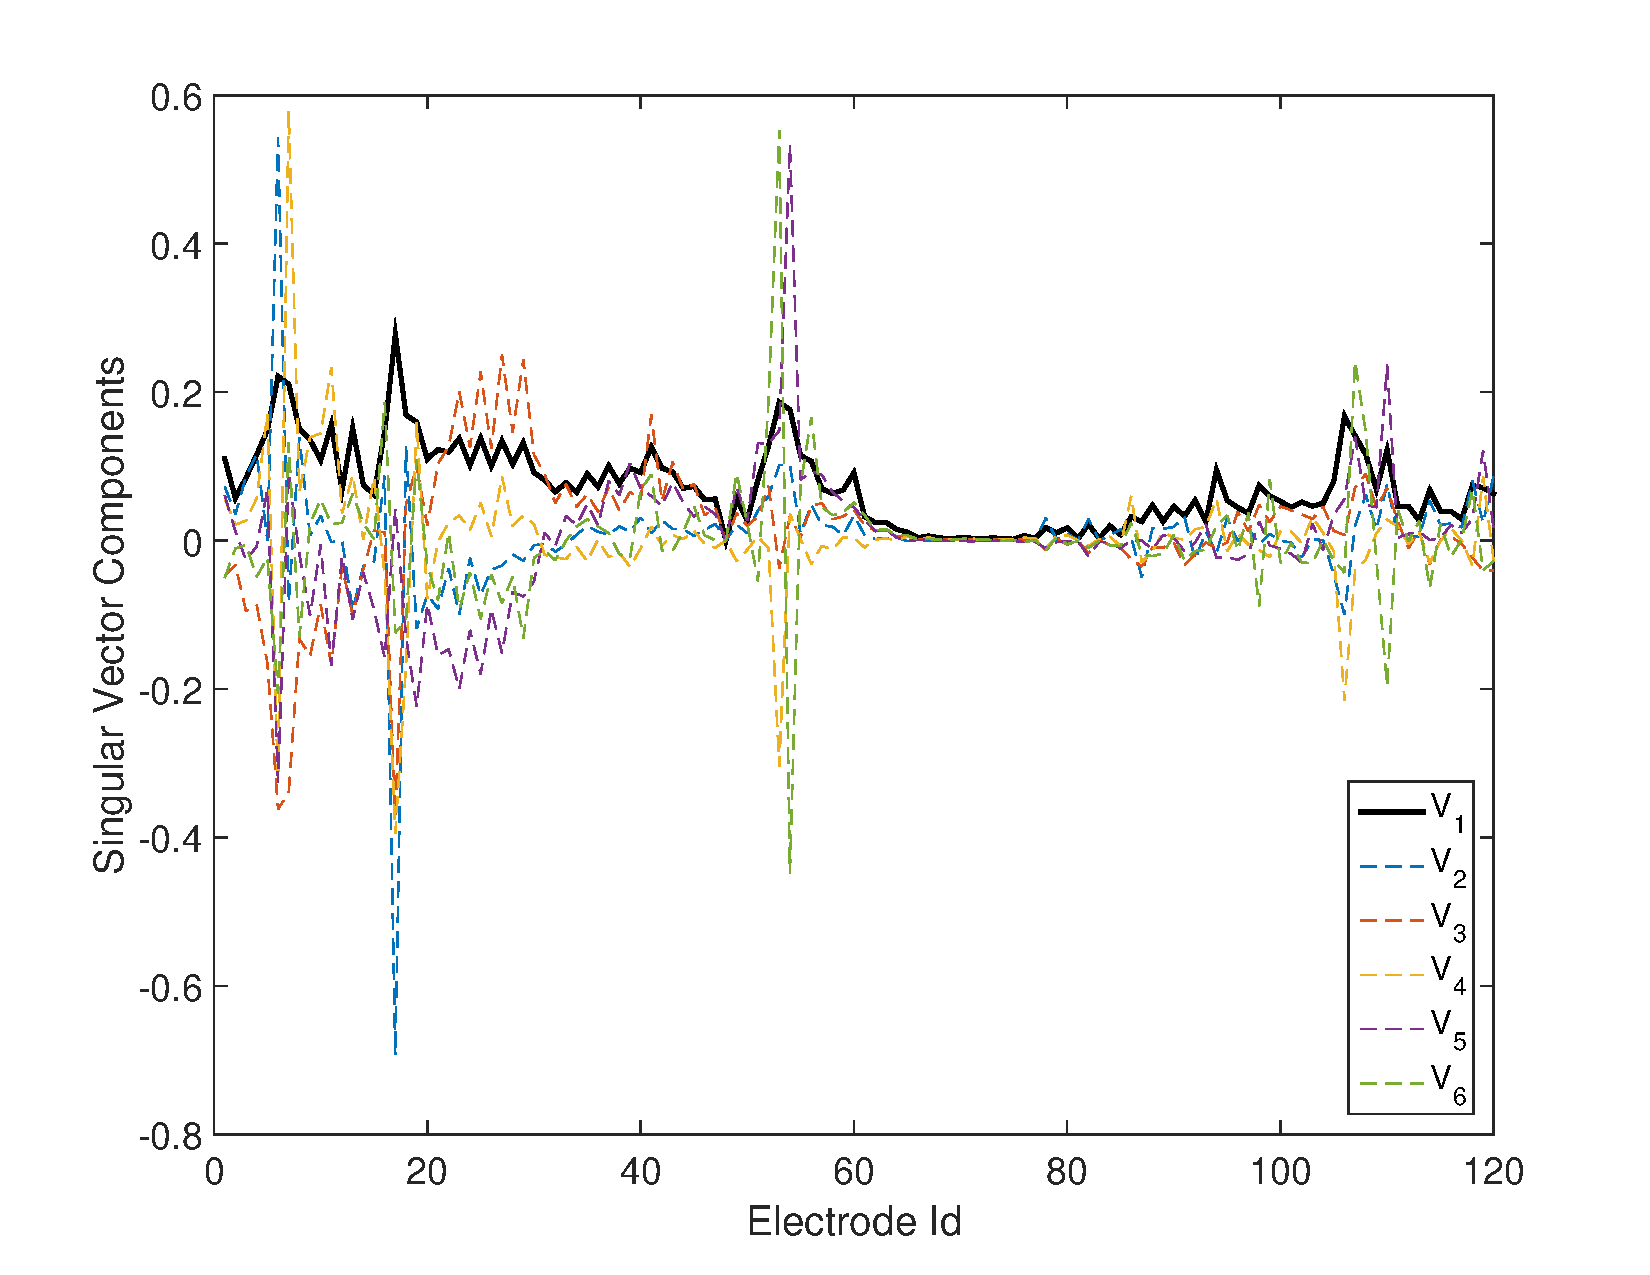
\includegraphics[trim=1.6cm 0.65cm 2.1cm 1.4cm, clip=true,width=0.475\linewidth]{./Figures/Fig7a.pdf}
       } %
    \subfigure[\tiny{SVD Electrode Analysis: Low Misfit Data}]{%
       \label{fig:DataQC_SVD_Elec_Good}
       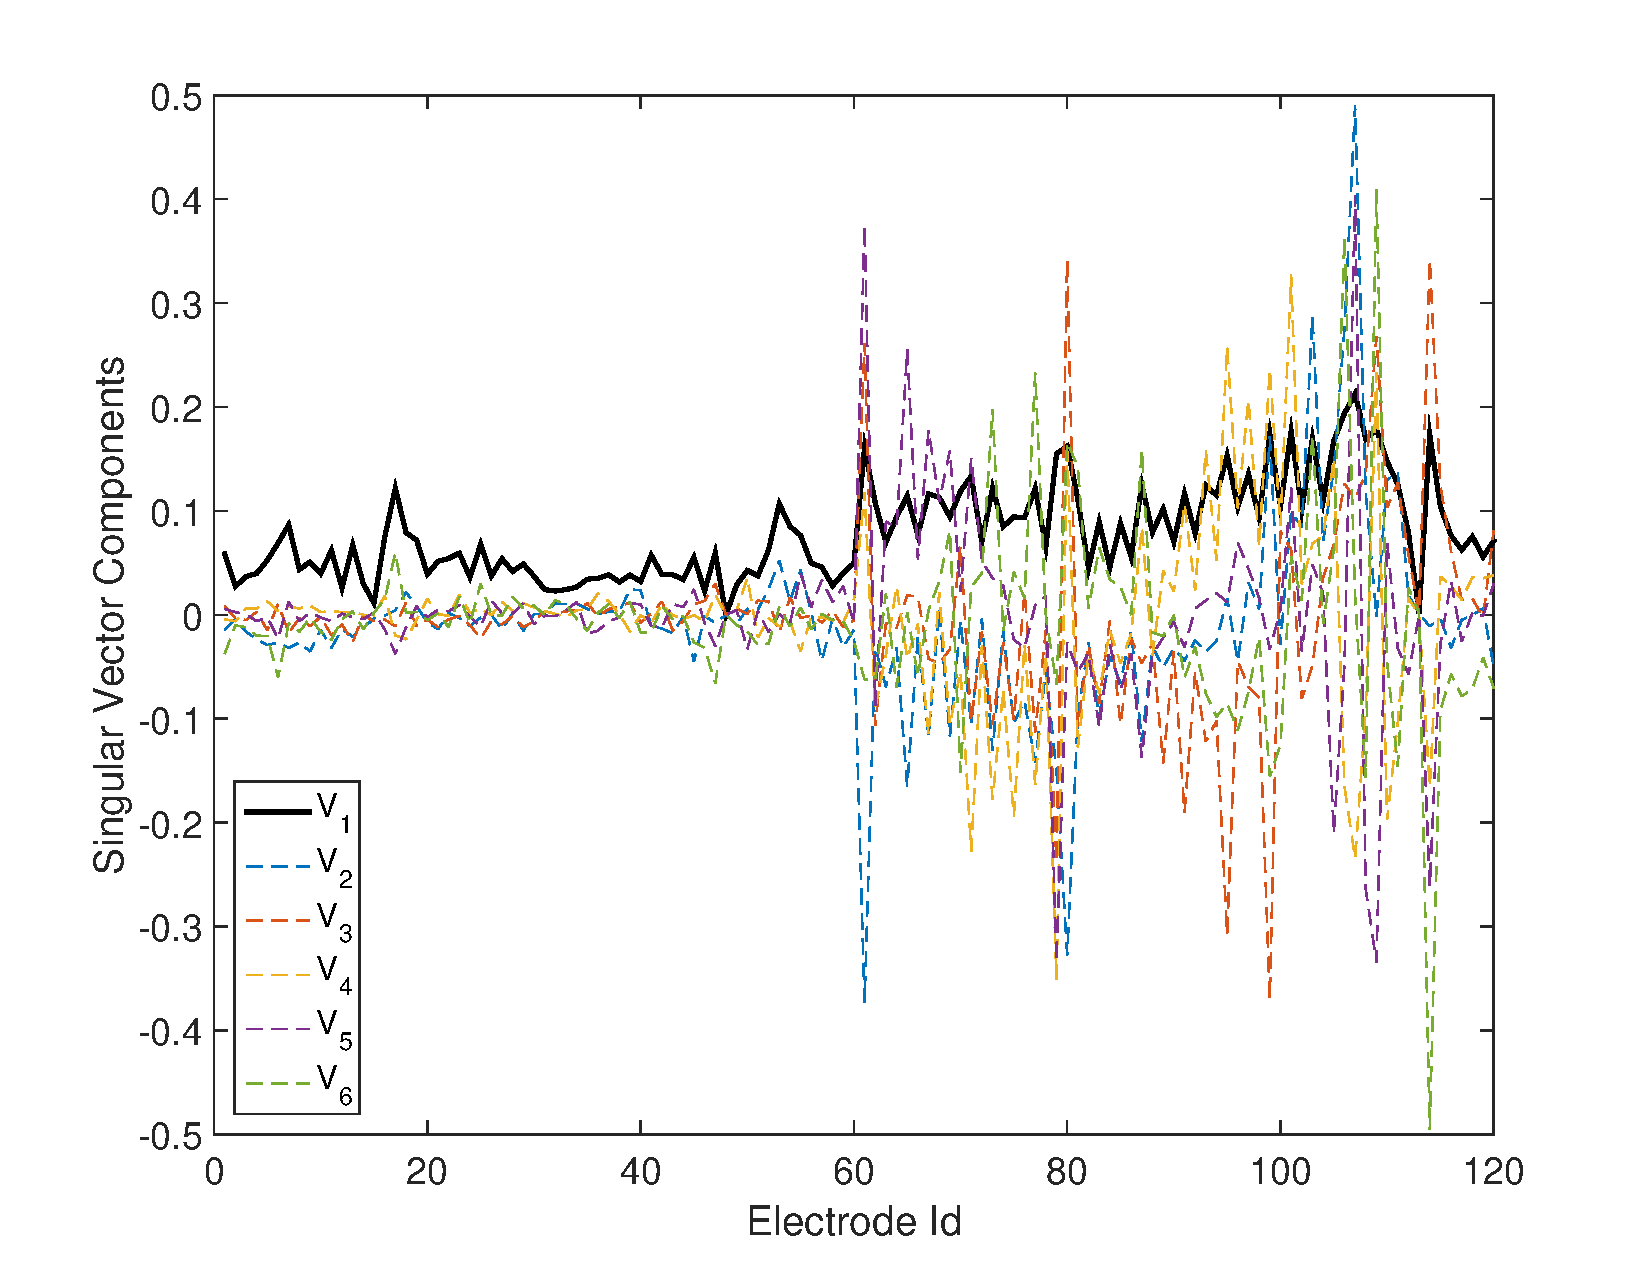
\includegraphics[trim=1.6cm 0.65cm 2.1cm 1.4cm, clip=true,width=0.475\linewidth]{./Figures/Fig7b.pdf}
       } \\%
    \subfigure[\tiny{SVD Cable Analysis: High Misfit Data}]{%
       \label{fig:DataQC_SVD_Cable_Bad}
       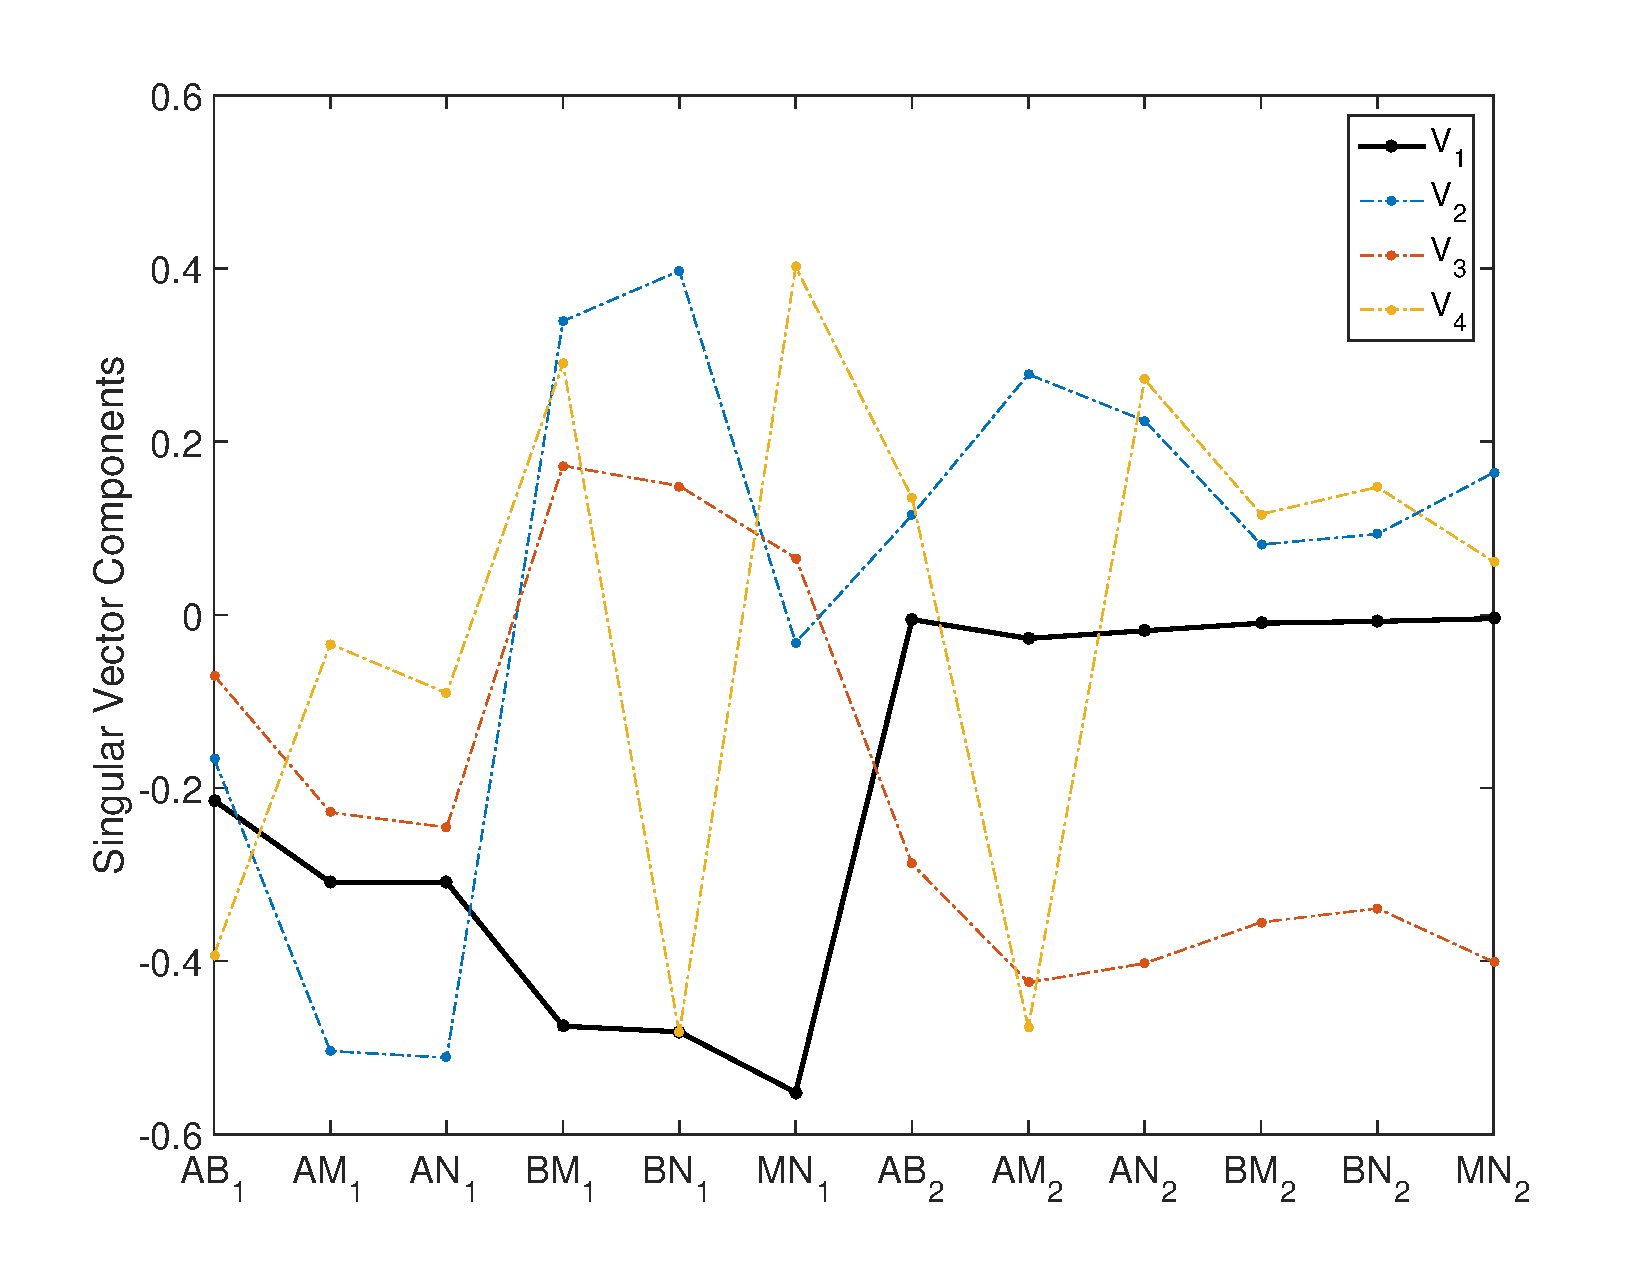
\includegraphics[trim=1.6cm 0.65cm 2cm 1.4cm, clip=true,width=0.475\linewidth]{./Figures/Fig7c.pdf}
       } %
    \subfigure[\tiny{SVD Cable Analysis: Low Misfit Data}]{%
       \label{fig:DataQC_SVD_Cable_Good}
       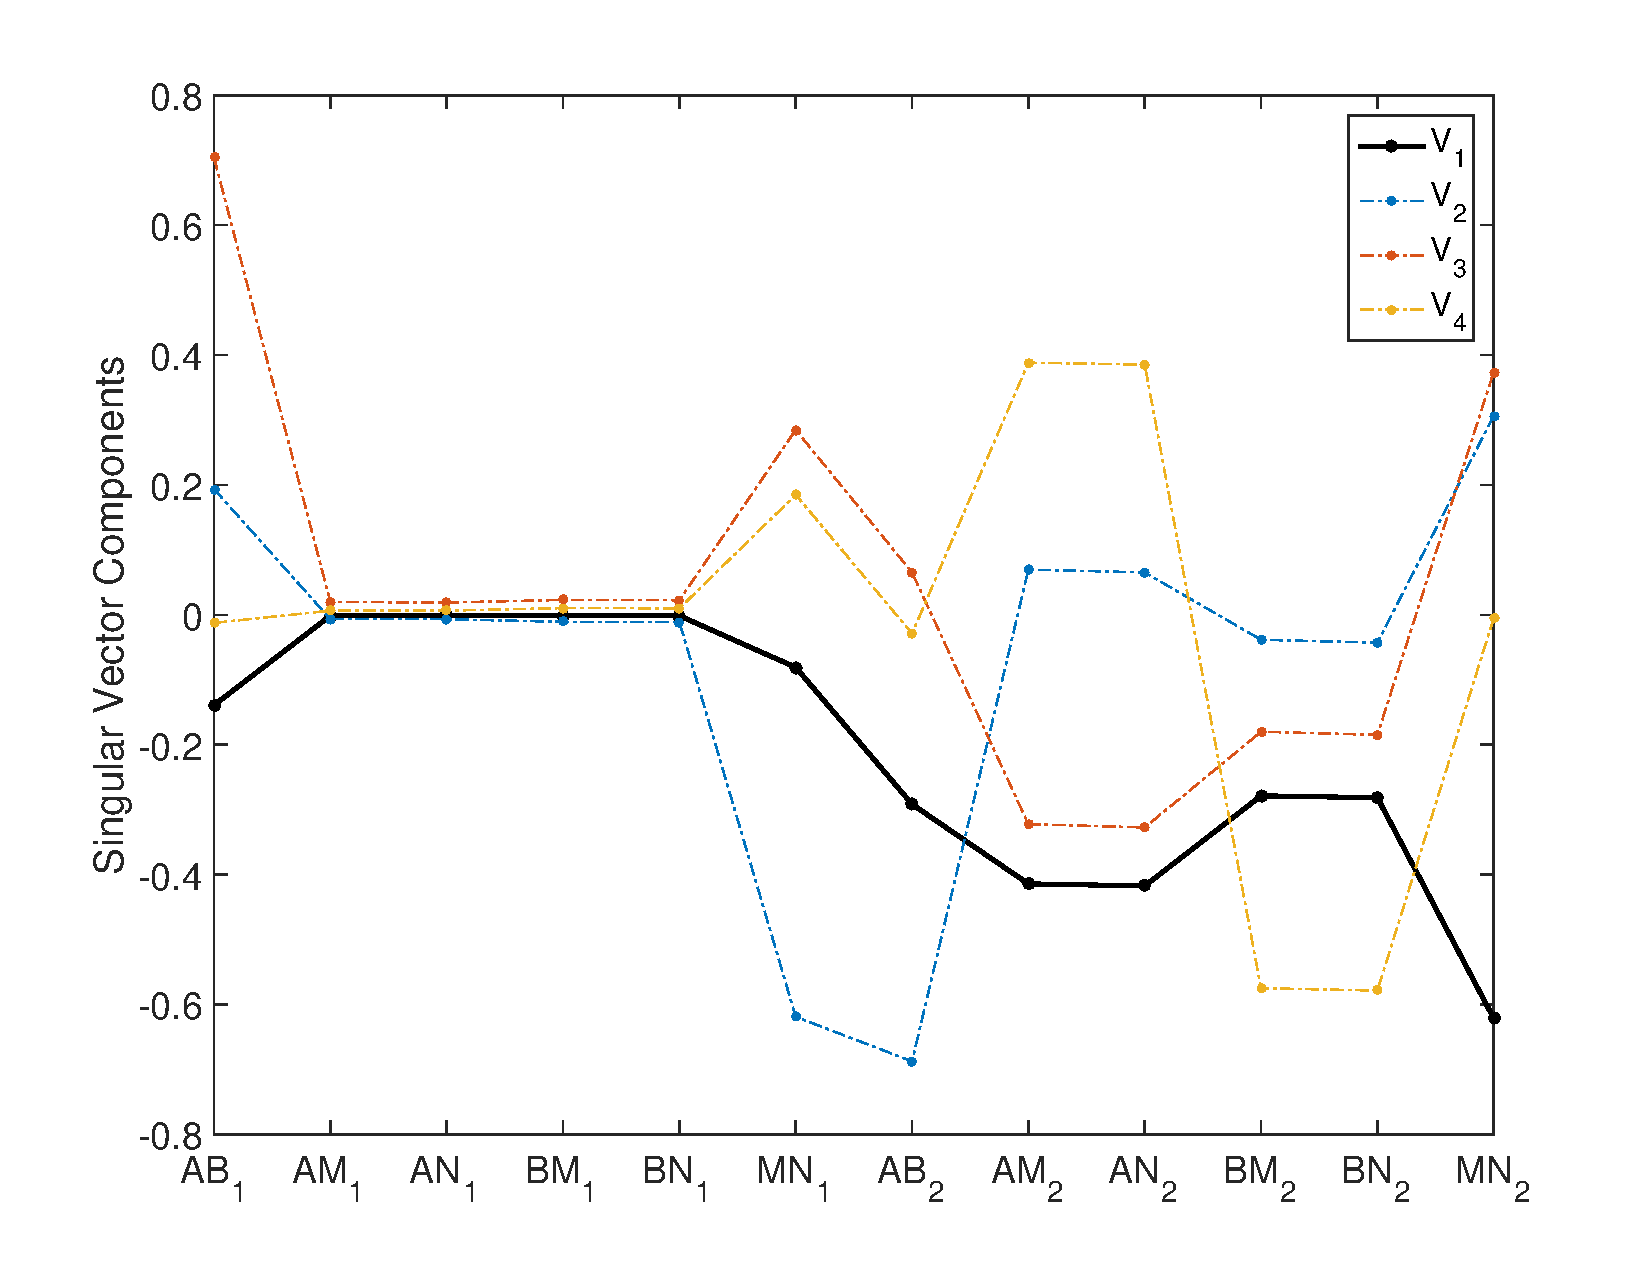
\includegraphics[trim=1.6cm 0.65cm 2cm 1.4cm, clip=true,width=0.475\linewidth]{./Figures/Fig7d.pdf}
       } \\%
    \end{center}
\caption{Panels \ref{fig:DataQC_SVD_Elec_Bad} and \ref{fig:DataQC_SVD_Elec_Good} show the singular vectors from the SVD factorization of the high and low data misfit indicator matrices, from the electrode SVD analysis while \ref{fig:DataQC_SVD_Cable_Bad} and \ref{fig:DataQC_SVD_Cable_Good} show the singular vectors from the cable SVD analysis. In both tests that first singular value is considerably larger that the remaining singular values. The results of these tests show that electrodes 1-60, connected with Cable 1, are more often associated with high misfit data than electrodes 61-120 or Cable 2.} 
\label{fig:DataQC_SVD_ElecCable}
\end{figure} 

Another indicator matrix was then made to look for correlations between data misfits and pairs of electrodes on the same cable. The same misfit level of 15 was used to differentiate between high and low data misfits. The results shown in Figures \ref{fig:DataQC_SVD_Cable_Bad} and \ref{fig:DataQC_SVD_Cable_Good} provide more evidence of a strong correlation between Cable 1 and high misfit data. 

Although it is possible to construct many other types of indicator matrices, these proved the most useful for this specific dataset. For other datasets, experimentation with different indicator matrices may prove useful. Having identified a potential problem within the switch cables or connection boxes which link electrodes 1-60 to the central control box we proceed to a boxplot analysis of misfit distributions for each electrode to see what additional information can be derived.     

Each column of the boxplot shows the distribution of misfits associated with data using the specified electrode as an A, B, M, or N electrode. Only the distribution of misfits associated with the M electrode IDs are shown in Figure \ref{fig:Boxplot_Misfit_vs_M_ElecID}. Here the first column of Figure \ref{fig:Boxplot_Full_DataMisfit_vs_MElecID} shows the distribution of all misfits associated with data which use electrode 1 as their M electrode. Since electrode noise levels may differ depending on whether an electrode is used as a current electrode or a potential electrode, similar boxplot graphs should also be made for A, B, and N electrode IDs. For all of the boxplots presented in the paper, the median is used to mark the midpoint of the distribution, the edges of the box correspond with the 25th and 75th percentiles, and the whiskers extend to the most extreme data within 2.7 standard deviations. Data points which fall outside of the whiskers are considered outliers and are plotted using a red +.

\begin{figure} [!ht]
    \begin{center}
    \subfigure[Full Dataset]{%
       \label{fig:Boxplot_Full_DataMisfit_vs_MElecID}
       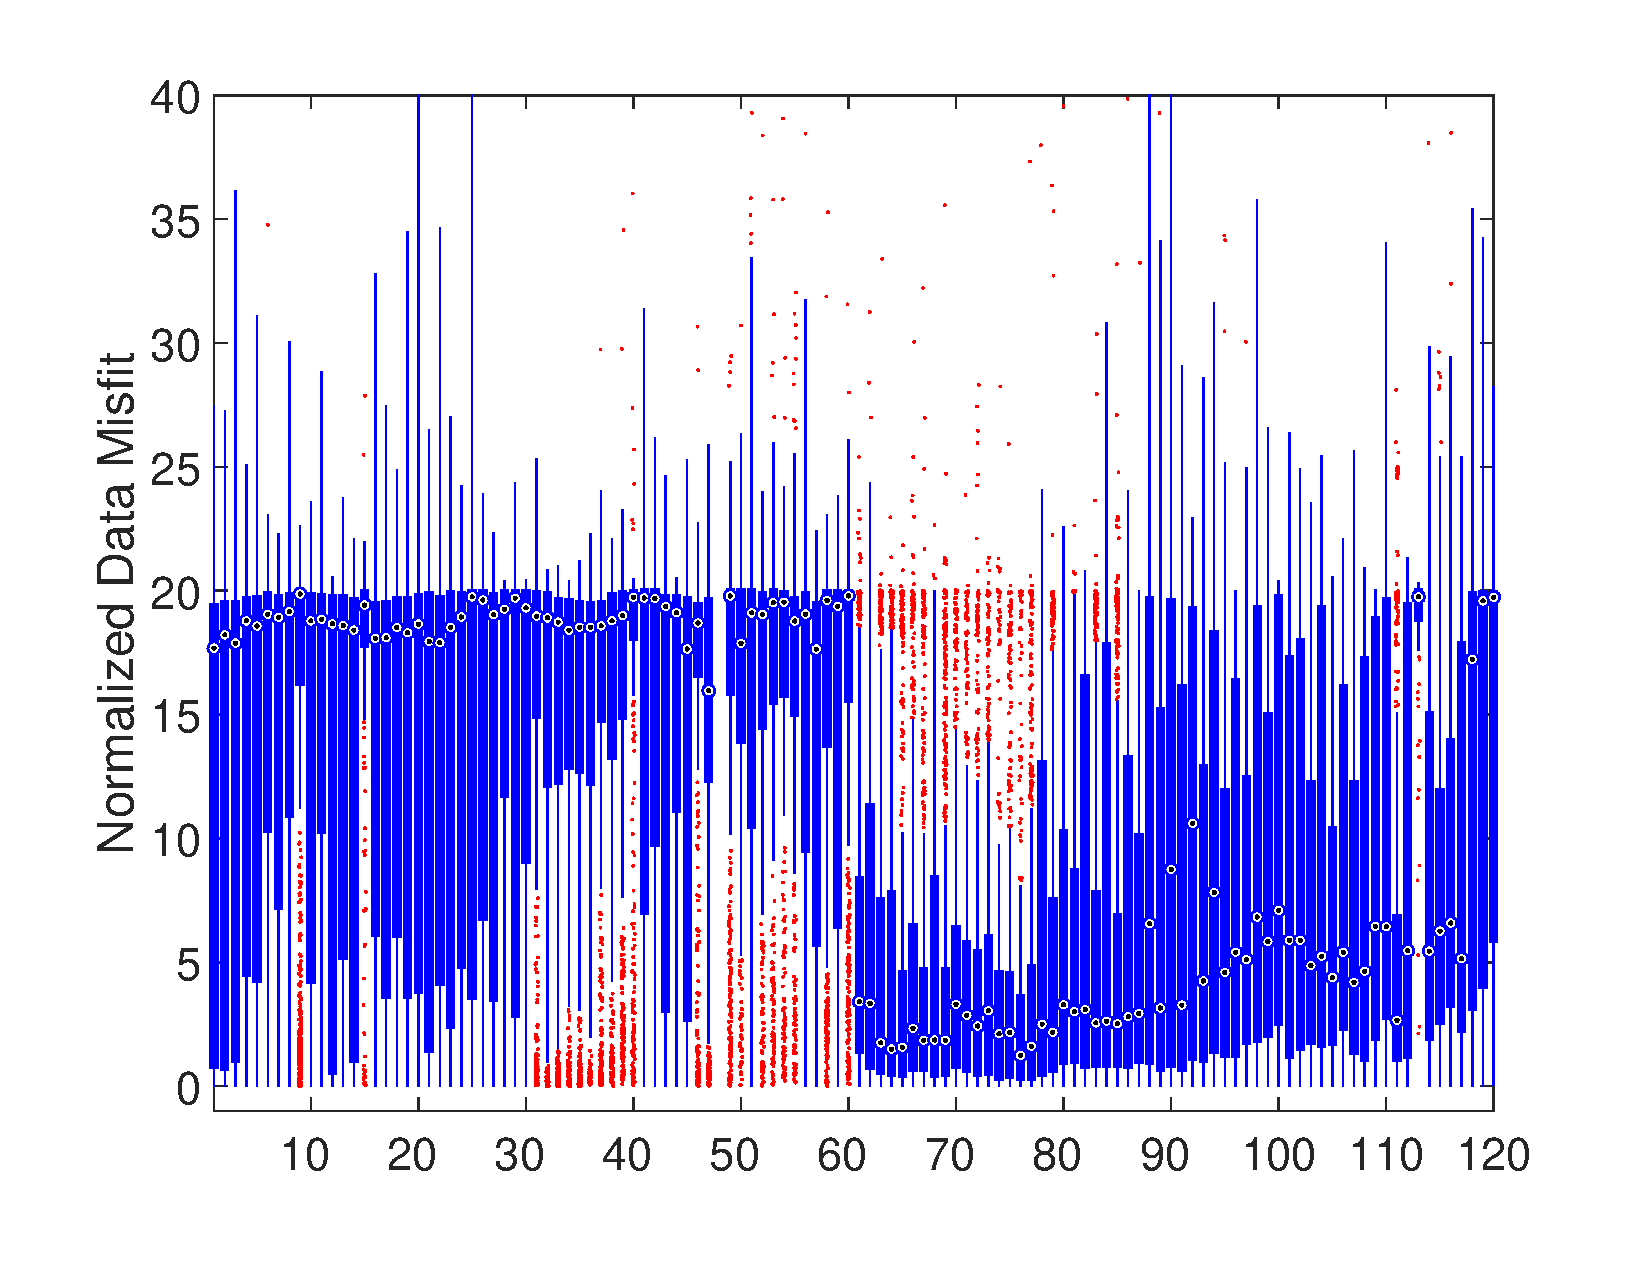
\includegraphics[trim=1.6cm 1.7cm 2cm 1.3cm, clip=true,width=0.475\linewidth]{./Figures/Fig8a.pdf}
       } %    
    \subfigure[ABMN-Cable 1]{%
       \label{fig:Boxplot_ABMN_Cable1_Misfit_vs_M_ElecID}
       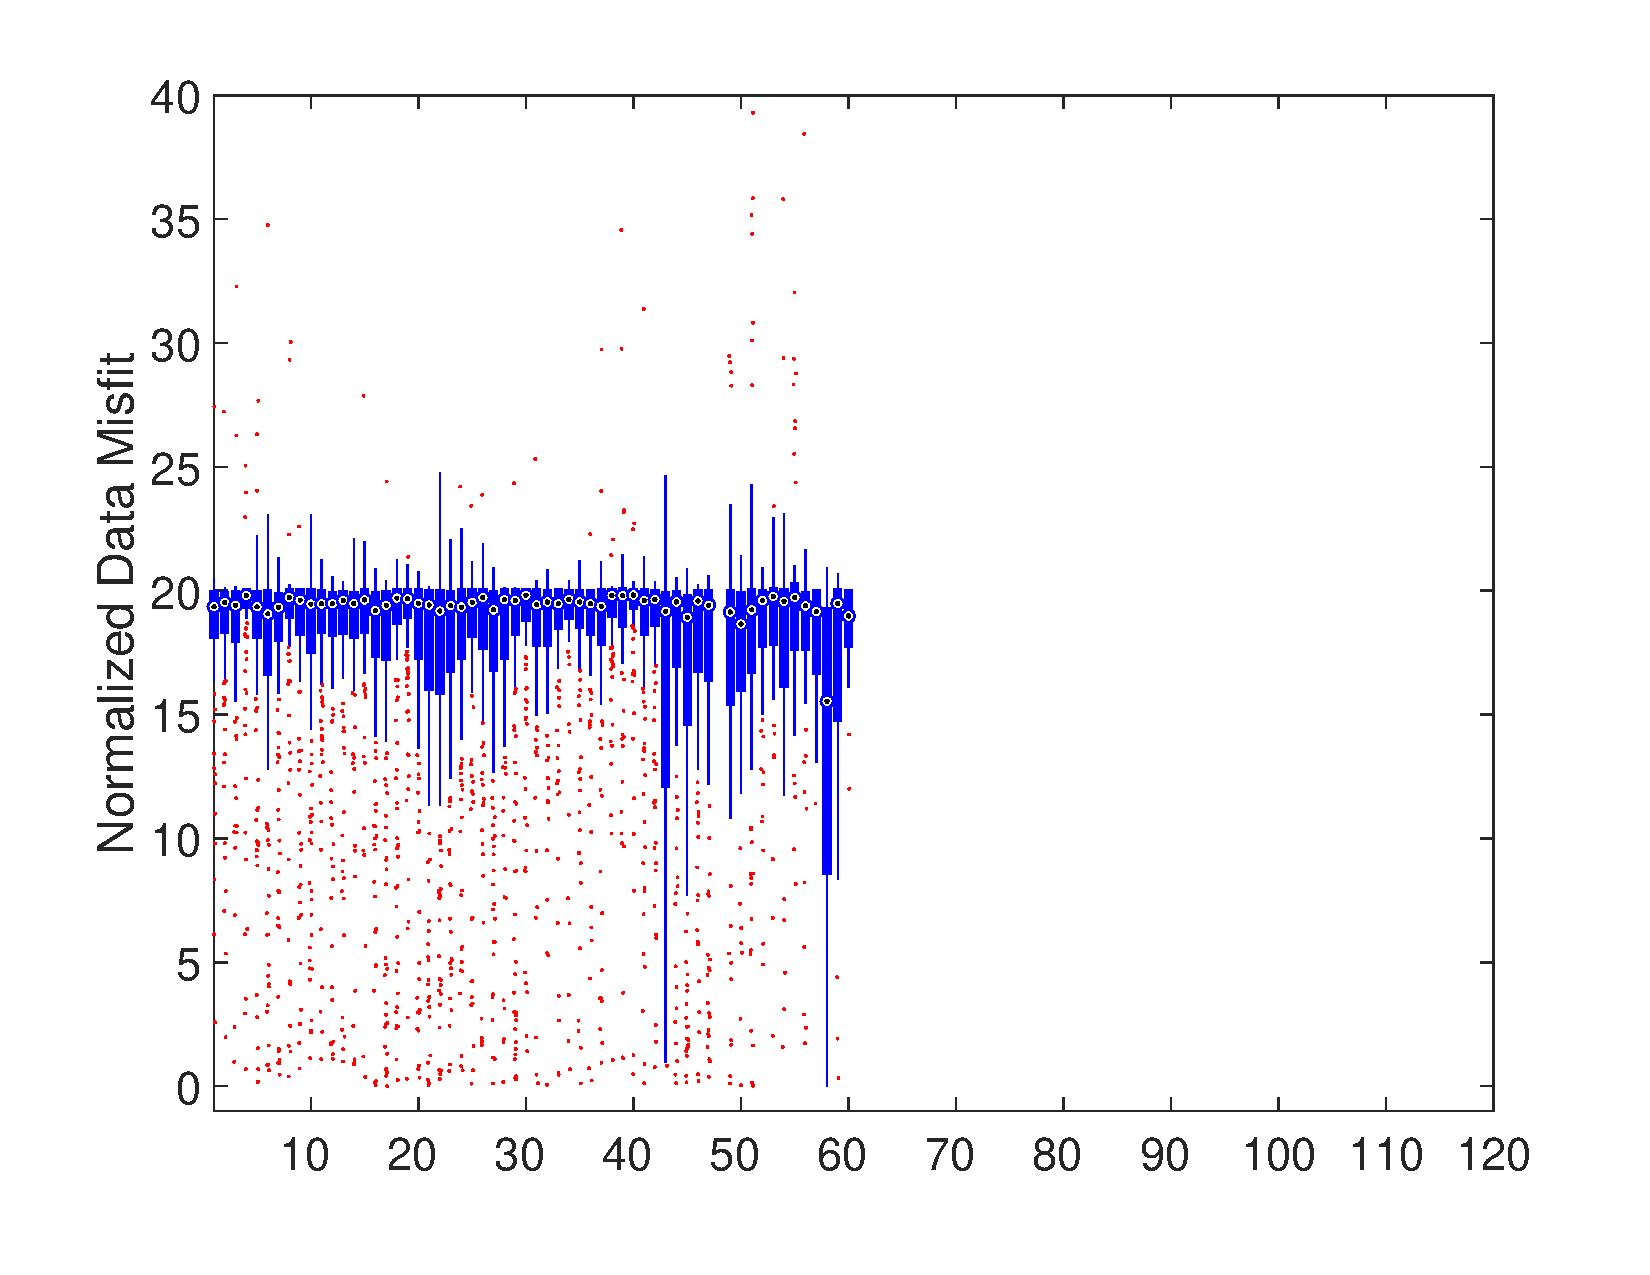
\includegraphics[trim=1.6cm 1.7cm 2cm 1.3cm, clip=true,width=0.475\linewidth]{./Figures/Fig8b.pdf}
       } \\%    
    \subfigure[ABMN-Cable 2]{%
       \label{fig:Boxplot_ABMN_Cable2_Misfit_vs_M_ElecID}
       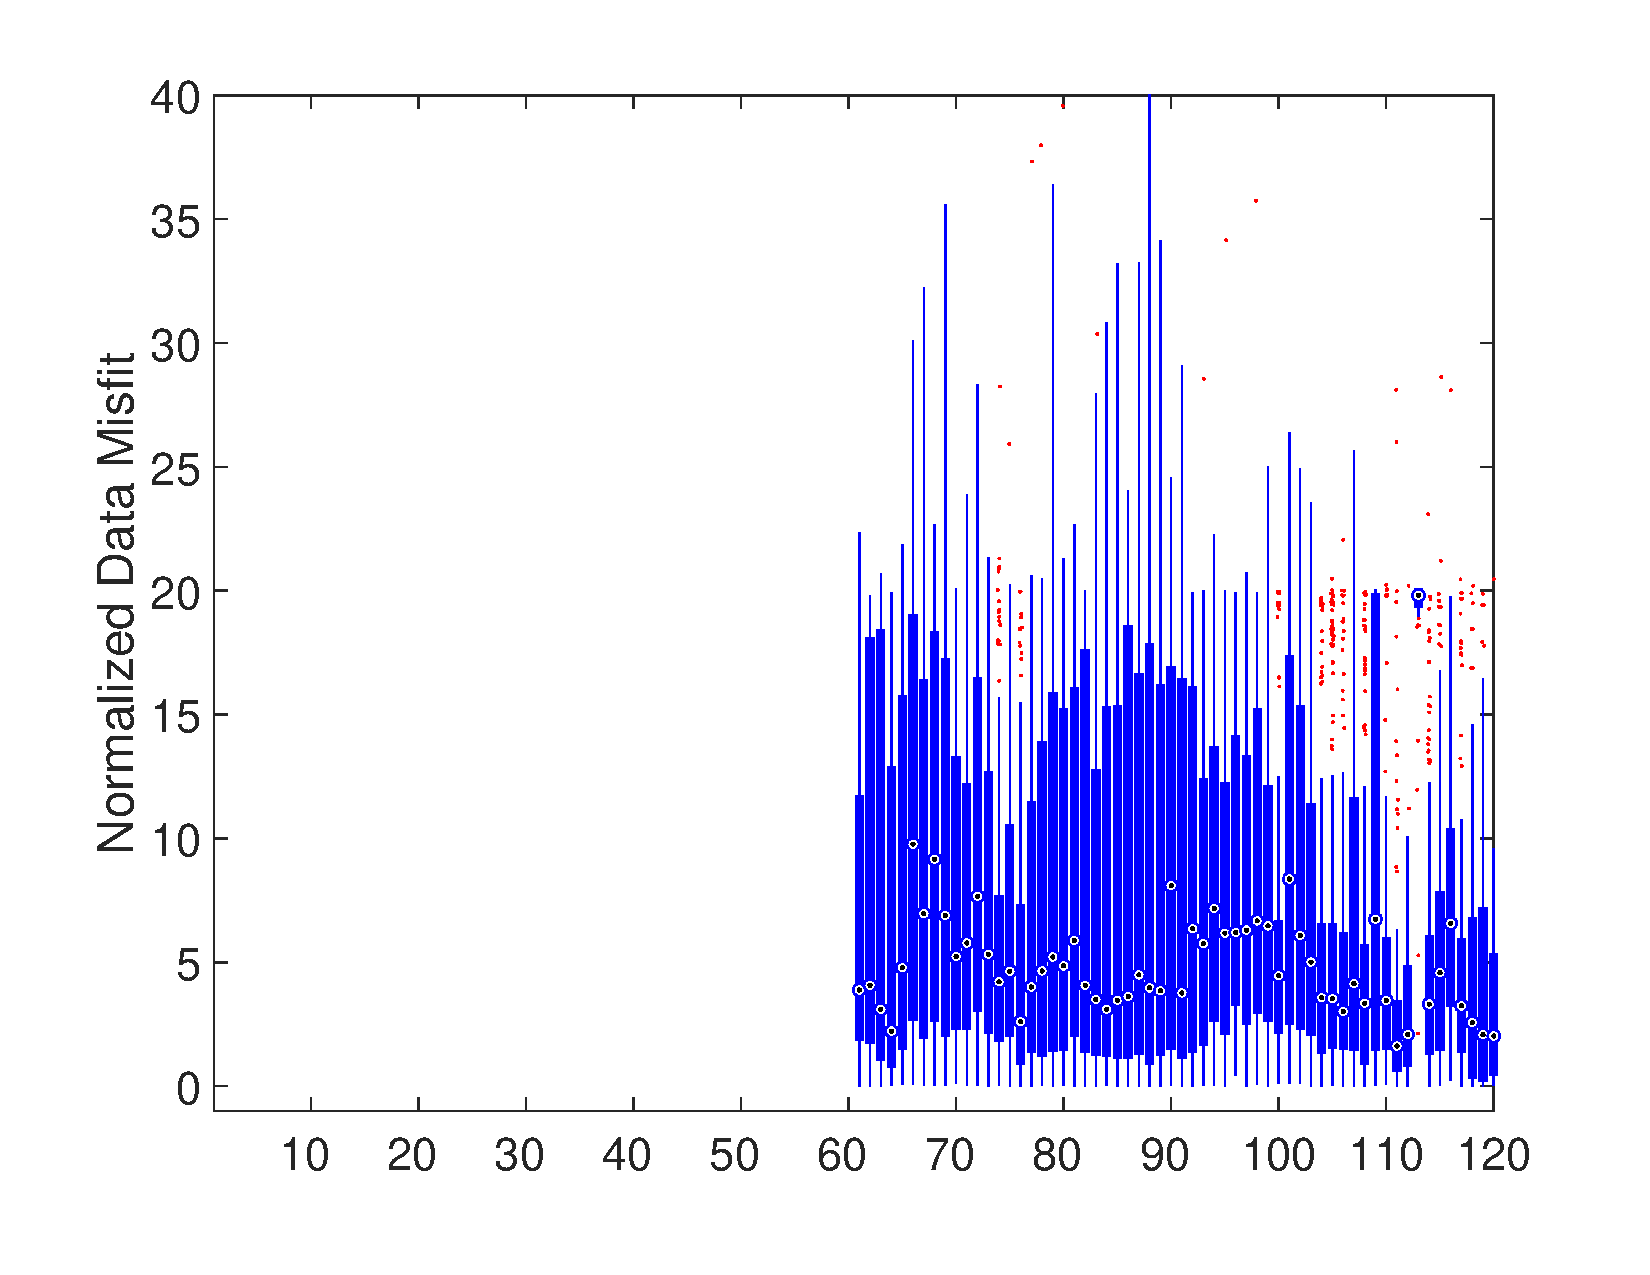
\includegraphics[trim=1.6cm 1.7cm 2cm 1.3cm, clip=true,width=0.475\linewidth]{./Figures/Fig8c.pdf}
       } %
    \subfigure[AB-Cable 1, MN-Cable 2]{%
       \label{fig:Boxplot_AB_Cable1_MN_Cable2_Misfit_vs_M_ElecID}
       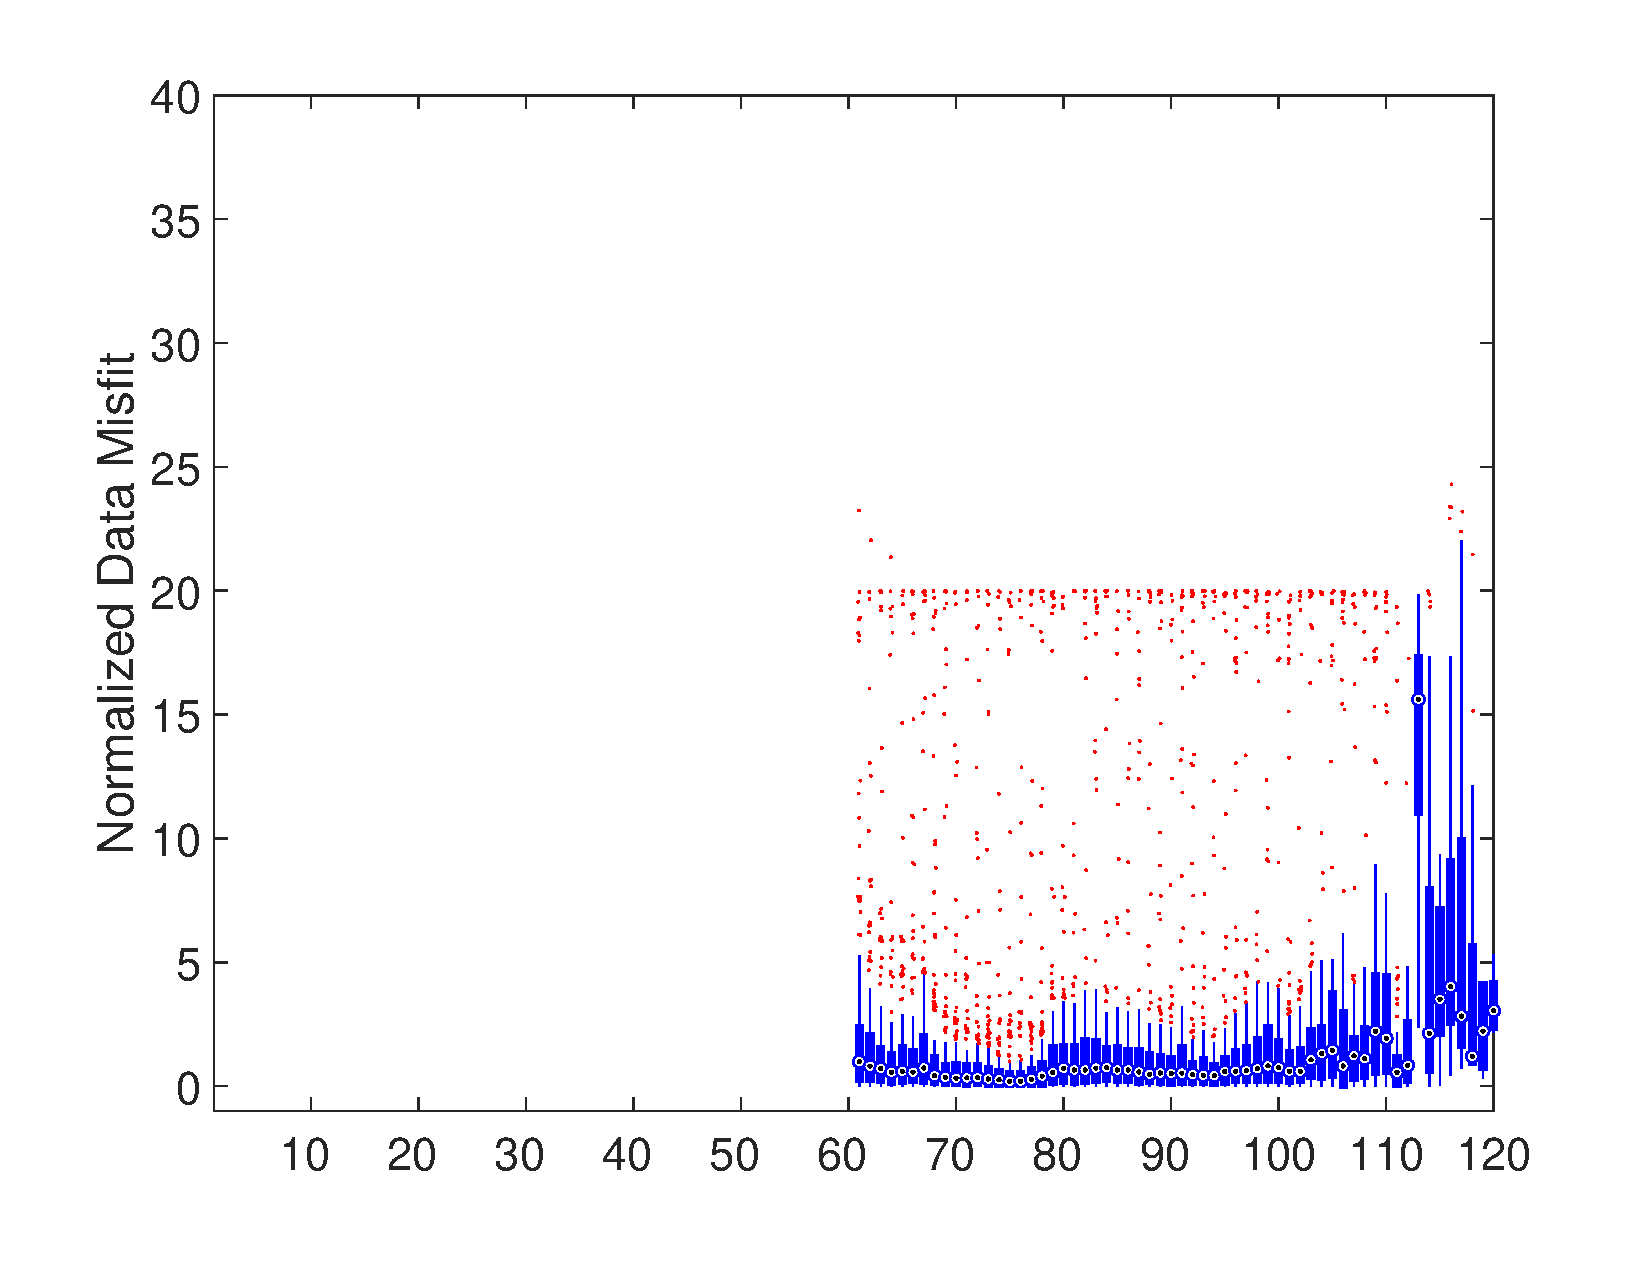
\includegraphics[trim=1.6cm 1.7cm 2cm 1.3cm, clip=true,width=0.475\linewidth]{./Figures/Fig8d.pdf}
       } \\%
    \subfigure[AB-Cable 2, MN-Cable 1]{%
       \label{fig:Boxplot_AB_Cable2_MN_Cable1_Misfit_vs_M_ElecID}
       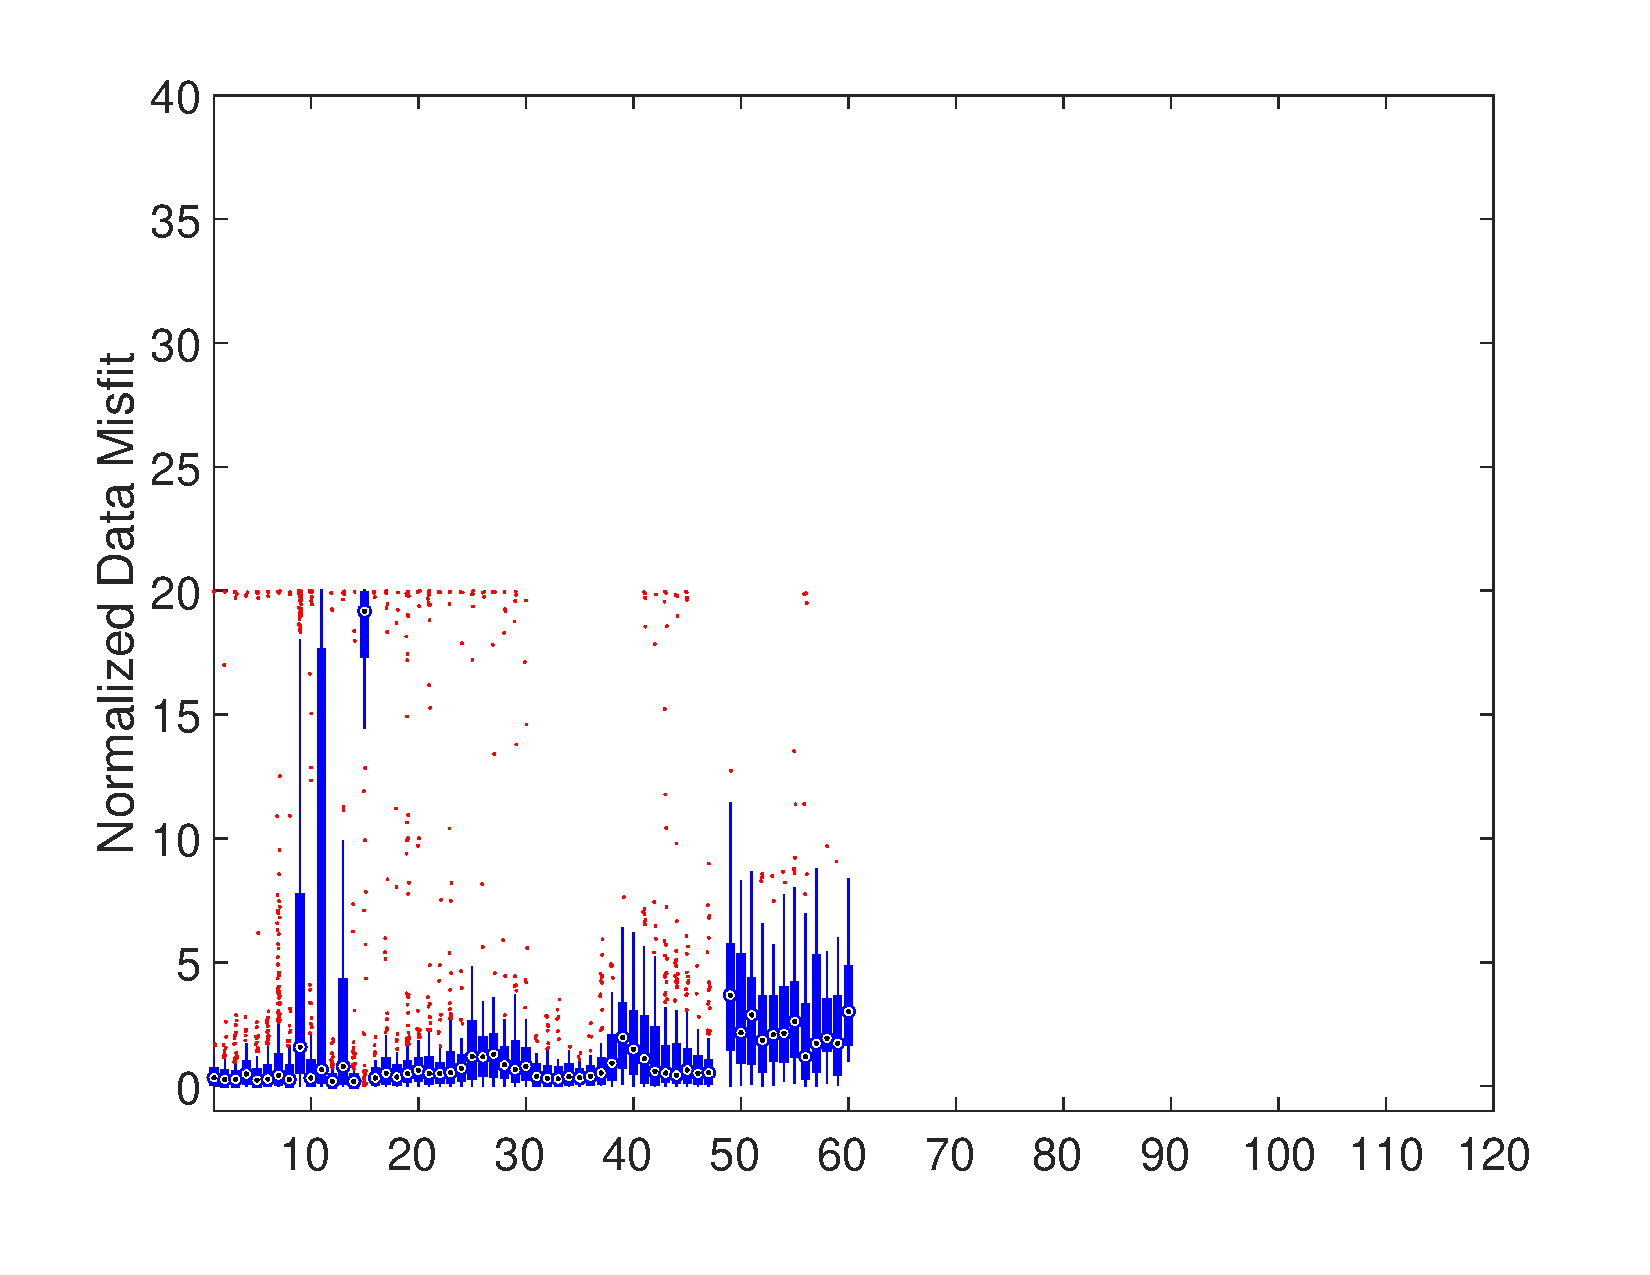
\includegraphics[trim=1.6cm 1.7cm 2cm 1.3cm, clip=true,width=0.475\linewidth]{./Figures/Fig8e.pdf}
       } %
    \subfigure[AB-Cable 1, MN-Mixed]{%
       \label{fig:Boxplot_AB_Cable1_MN_Mixed_Misfit_vs_M_ElecID}
       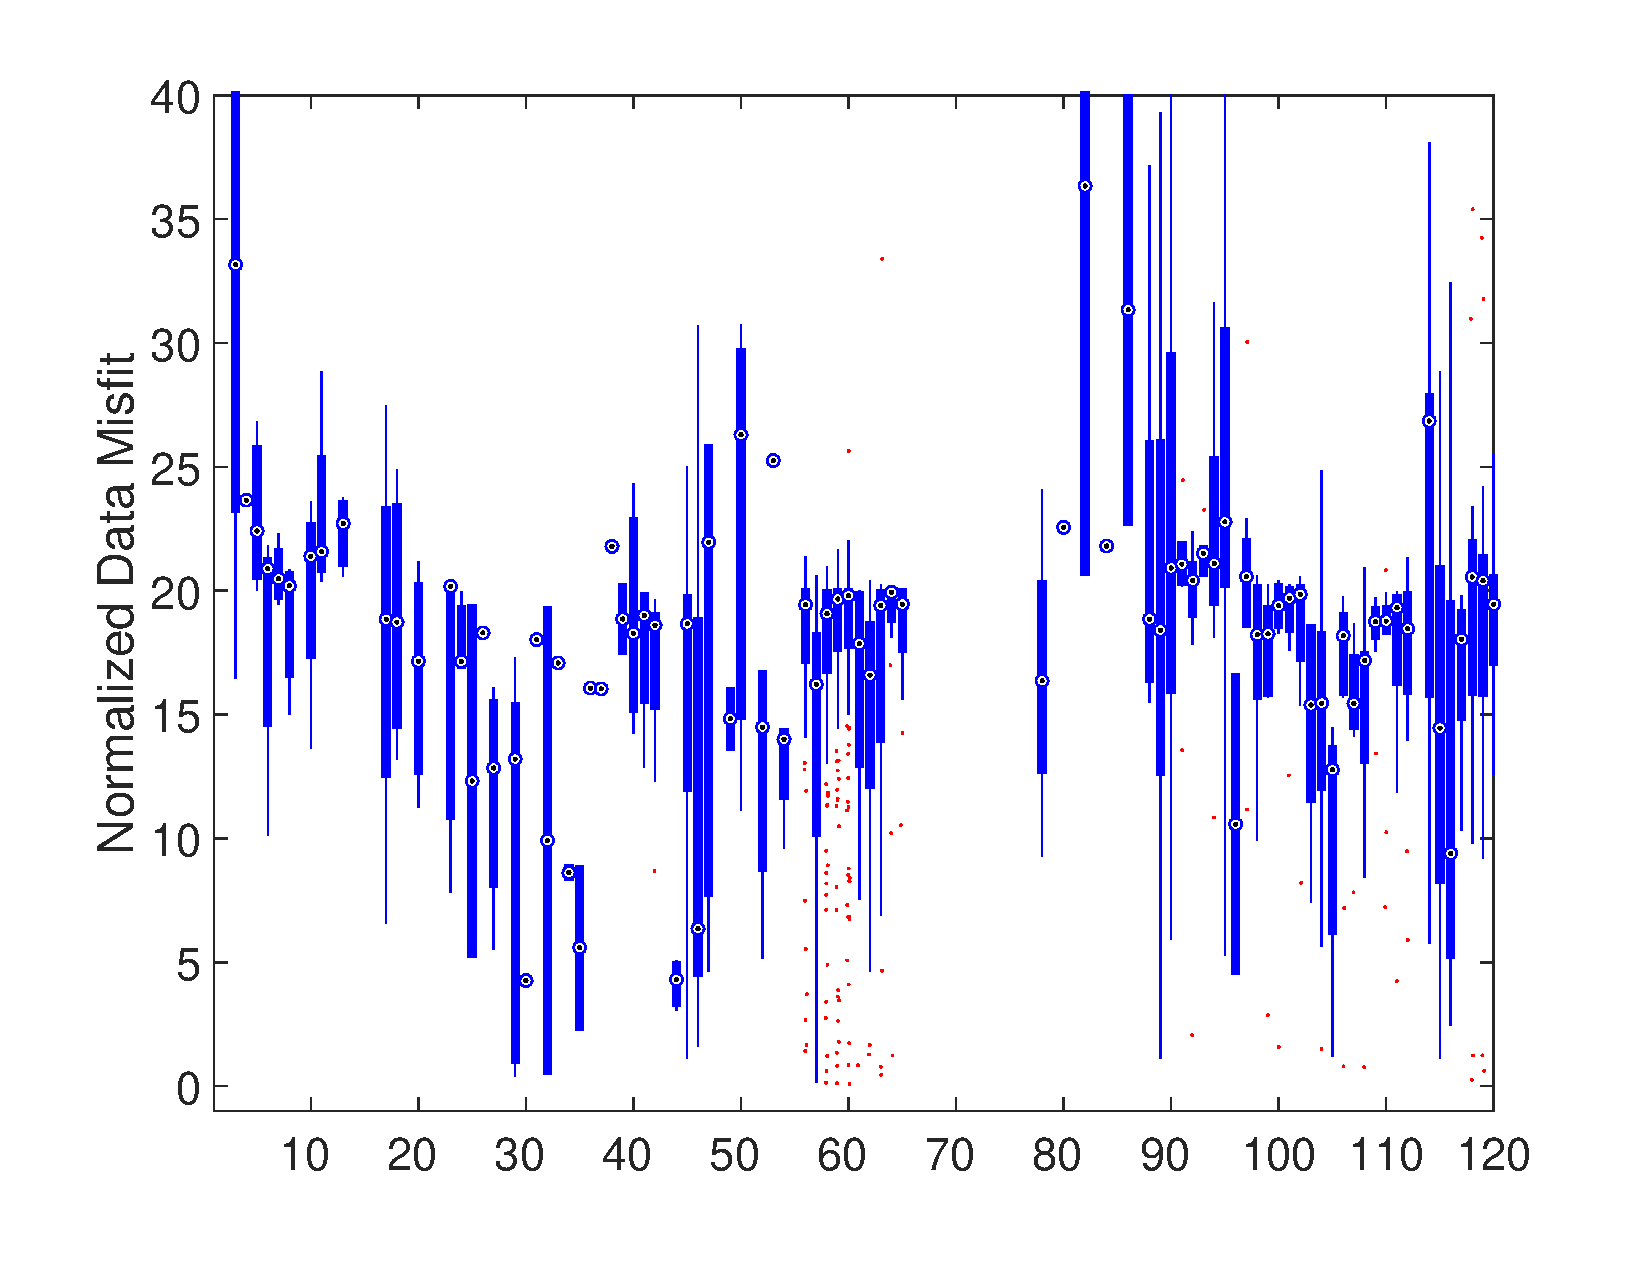
\includegraphics[trim=1.6cm 1.7cm 2cm 1.3cm, clip=true,width=0.475\linewidth]{./Figures/Fig8f.pdf}
       } \\%    
    \subfigure[AB-Cable 2, MN-Mixed]{%
       \label{fig:Boxplot_AB_Cable2_MN_Mixed_Misfit_vs_M_ElecID}
       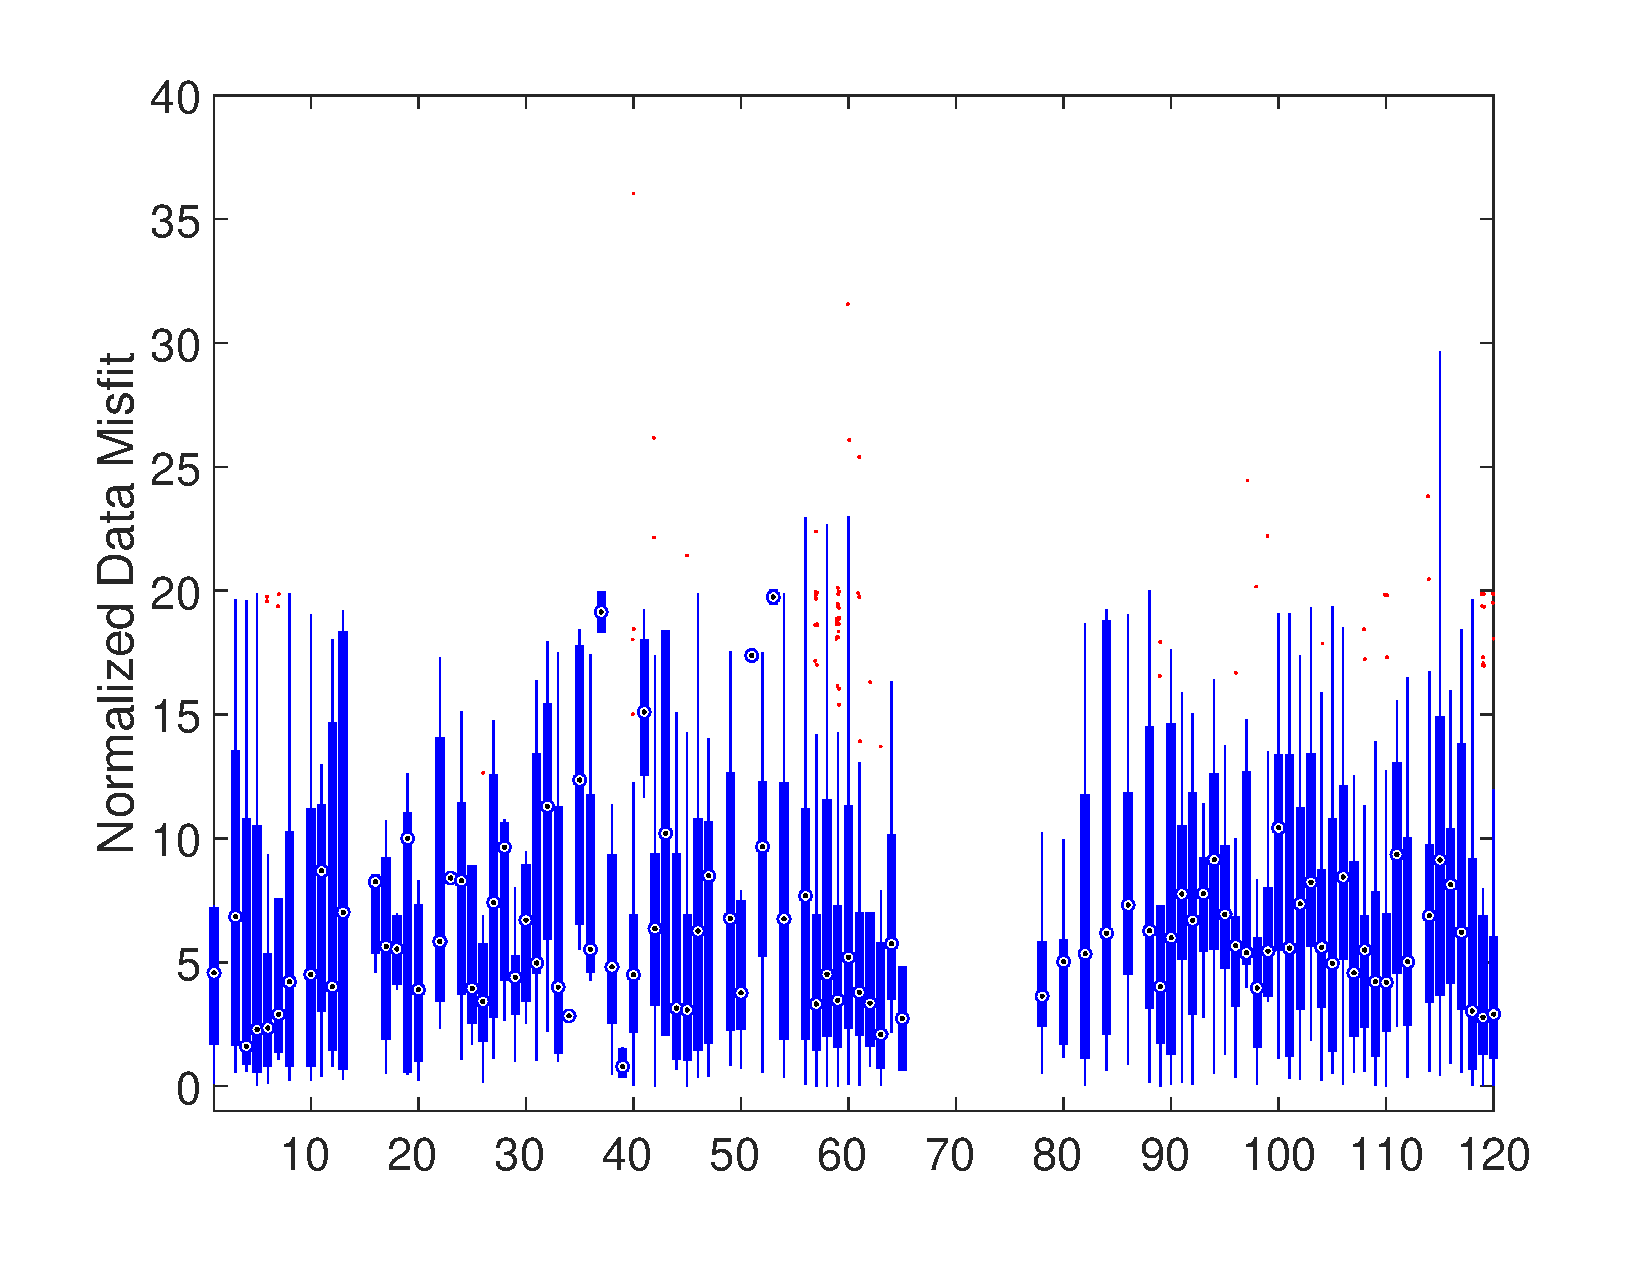
\includegraphics[trim=1.6cm 1.7cm 2cm 1.3cm, clip=true,width=0.475\linewidth]{./Figures/Fig8g.pdf}
       } %
    \subfigure[AB-Mixed, MN-Cable 1]{%
       \label{fig:Boxplot_AB_Mixed_MN_Cable1_Misfit_vs_M_ElecID}
       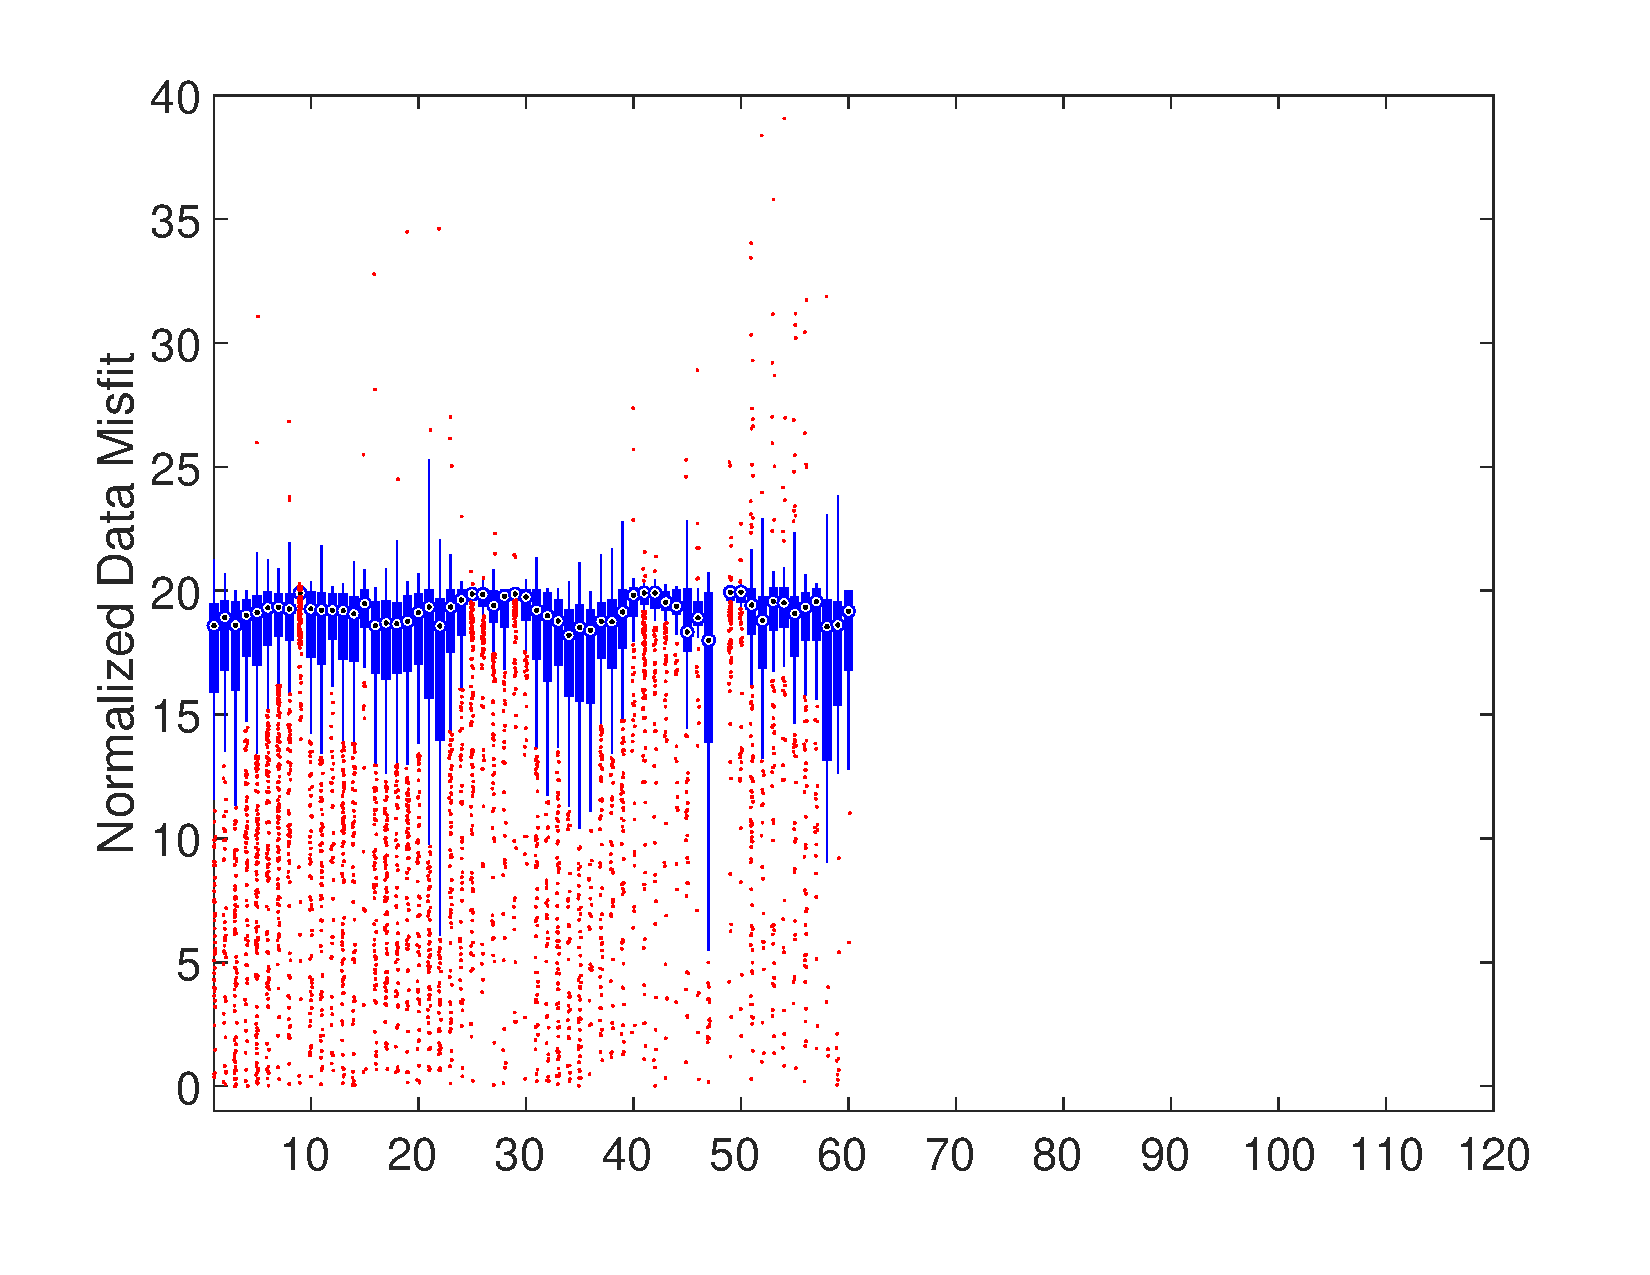
\includegraphics[trim=1.6cm 1.7cm 2cm 1.3cm, clip=true,width=0.475\linewidth]{./Figures/Fig8h.pdf}
       } \\%
    \subfigure[AB-Mixed, MN-Cable 2]{%
       \label{fig:Boxplot_AB_Mixed_MN_Cable2_Misfit_vs_M_ElecID}
       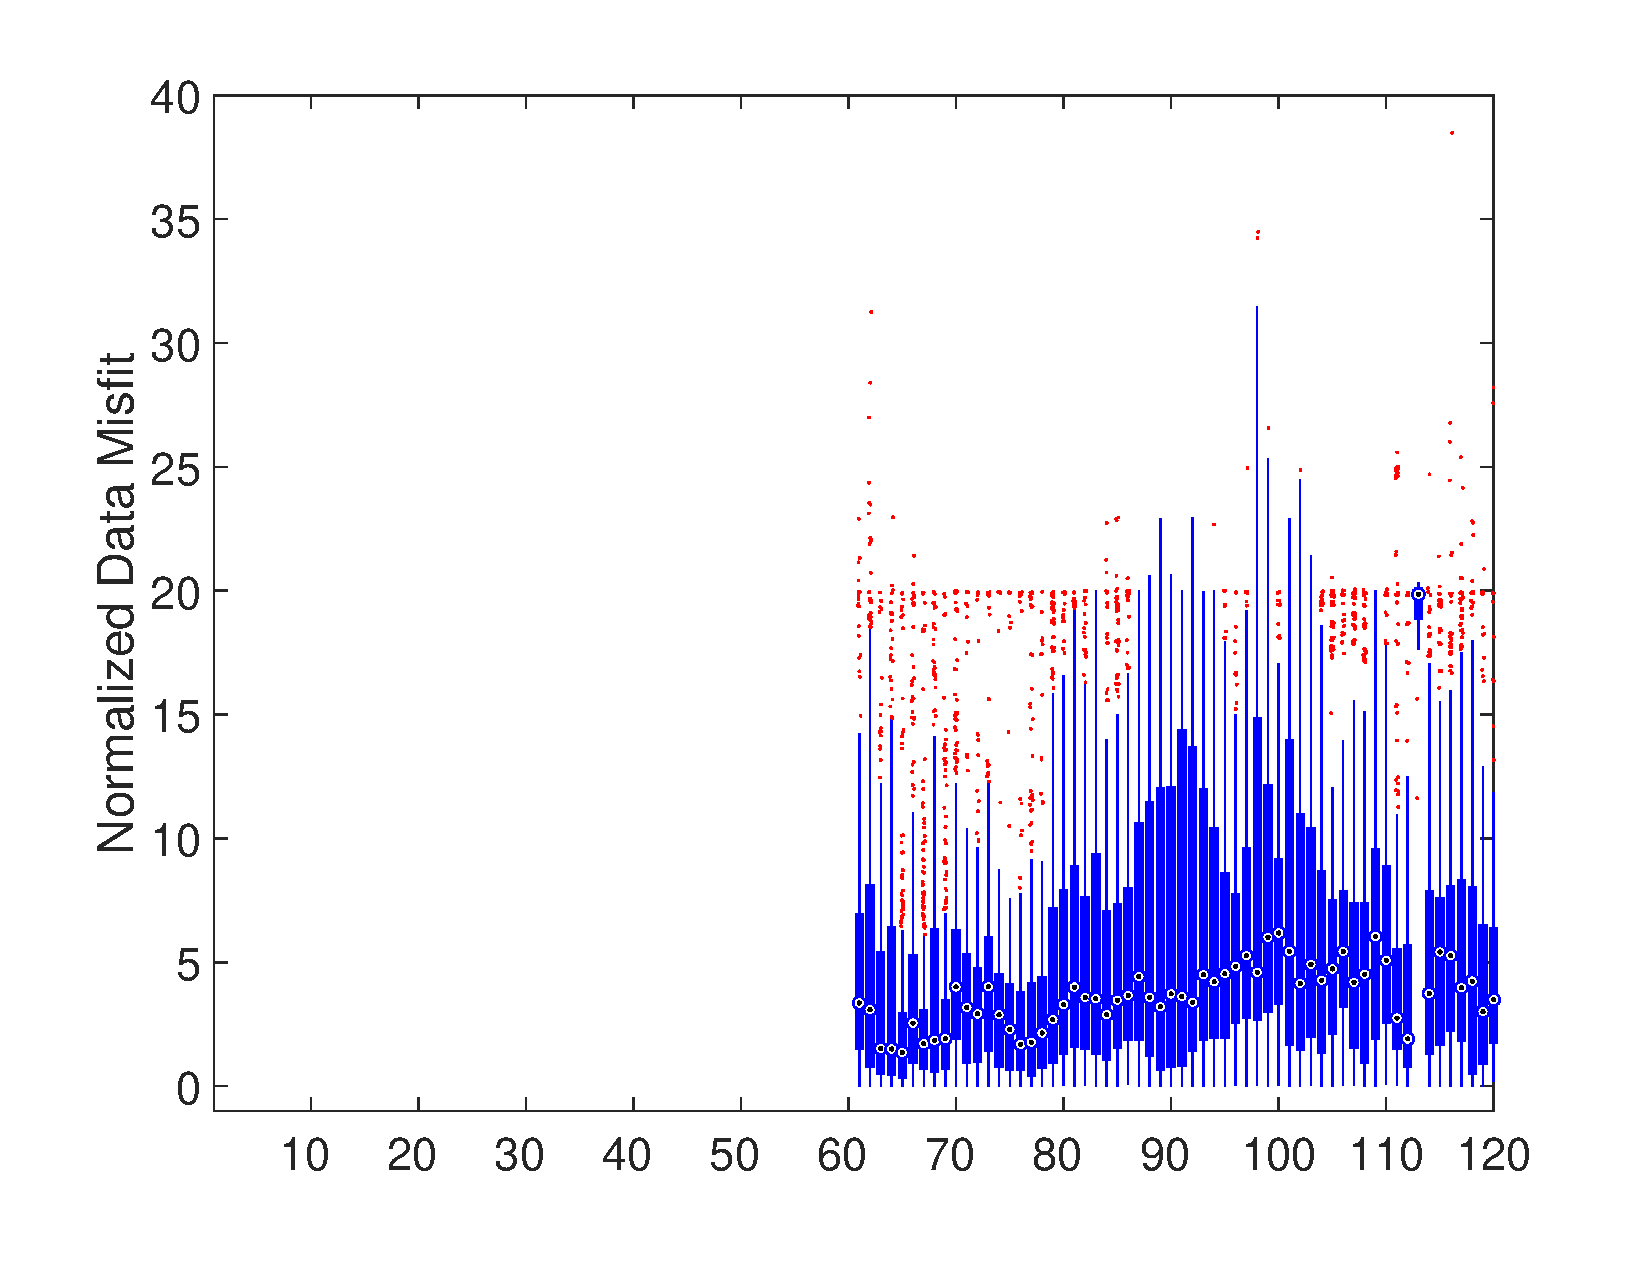
\includegraphics[trim=1.6cm 1.7cm 2cm 1.3cm, clip=true,width=0.475\linewidth]{./Figures/Fig8i.pdf}
       } %
    \subfigure[AB-Mixed, MN-Mixed]{%
       \label{fig:Boxplot_AB_Mixed_MN_Mixed_Misfit_vs_M_ElecID}
       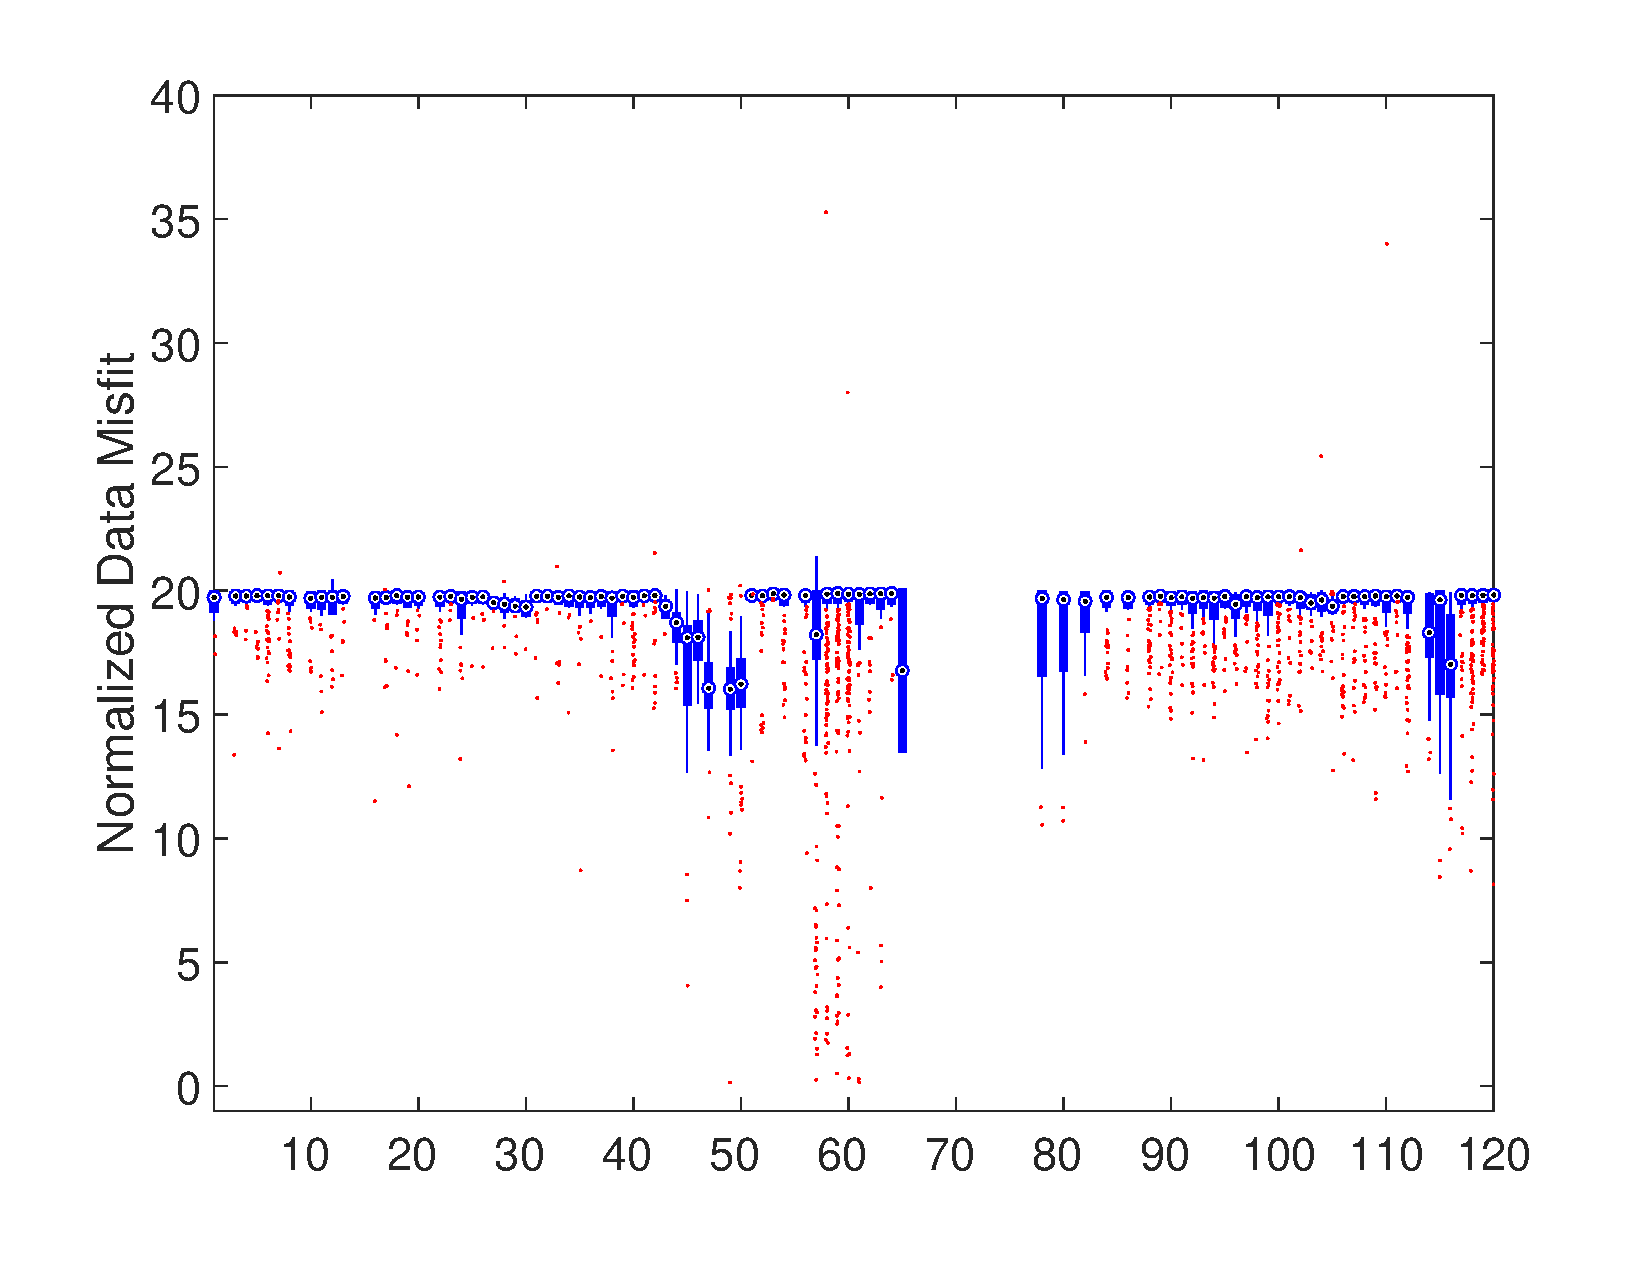
\includegraphics[trim=1.6cm 1.7cm 2cm 1.3cm, clip=true,width=0.475\linewidth]{./Figures/Fig8j.pdf}
       } %
    \end{center}
\caption{A series of boxplot diagrams which show the distribution of the normalized data misfits associated with each electrode when it is used as an M potential electrode. These plots clearly show that current leakages in the switch cables or connection boxes which link the electrodes to the central control box are the primary source of noise in this dataset. The current leakages are more severe in Cable 1 which connects electrodes 1-60 than in Cable 2 which connects electrodes 61-120.}
\label{fig:Boxplot_Misfit_vs_M_ElecID}
\end{figure}

When we analyze the full dataset using these boxplot graphs (see Figure \ref{fig:Boxplot_Full_DataMisfit_vs_MElecID}) there is a distinct difference in the noise levels associated with electrodes 1-60 and 61-120. The fact that this dichotomy correlates perfectly with the separation between Cables 1 and 2 provides strong evidence suggesting that our data is highly contaminated by electrical noise associated with current leakages. 

By separating the data into subsets based on which cable the TX dipole and RX dipole are on we produce plots \ref{fig:Boxplot_ABMN_Cable1_Misfit_vs_M_ElecID}-\ref{fig:Boxplot_AB_Mixed_MN_Mixed_Misfit_vs_M_ElecID} which prove that current leakages between the TX lines and RX lines are the primary source of noise within the data. This is most clearly illustrated by the low median misfit values attained when the TX and RX electrodes are on separate cables (see plots \ref{fig:Boxplot_AB_Cable1_MN_Cable2_Misfit_vs_M_ElecID} and \ref{fig:Boxplot_AB_Cable2_MN_Cable1_Misfit_vs_M_ElecID}) compared to the uniformly high median misfits observed when the TX and RX electrodes are both on the same cable (see plots \ref{fig:Boxplot_ABMN_Cable1_Misfit_vs_M_ElecID} and \ref{fig:Boxplot_ABMN_Cable2_Misfit_vs_M_ElecID}). Plots \ref{fig:Boxplot_ABMN_Cable1_Misfit_vs_M_ElecID} and \ref{fig:Boxplot_ABMN_Cable2_Misfit_vs_M_ElecID} also show that the current leakages within Cable 1 are more severe than those in Cable 2. This claim is further supported by the fact that the data is most highly contaminated when at least one of the TX and RX electrodes are on Cable 1 (see plots \ref{fig:Boxplot_AB_Mixed_MN_Cable1_Misfit_vs_M_ElecID} and \ref{fig:Boxplot_AB_Mixed_MN_Cable2_Misfit_vs_M_ElecID}). These findings support the general results of the SVD analysis, but more clearly show the scope of the problem.

\begin{figure} [!ht]
    \begin{center}
    \subfigure{%
       \label{fig:CableSplit_Cluster_PropBoxPlot1}
       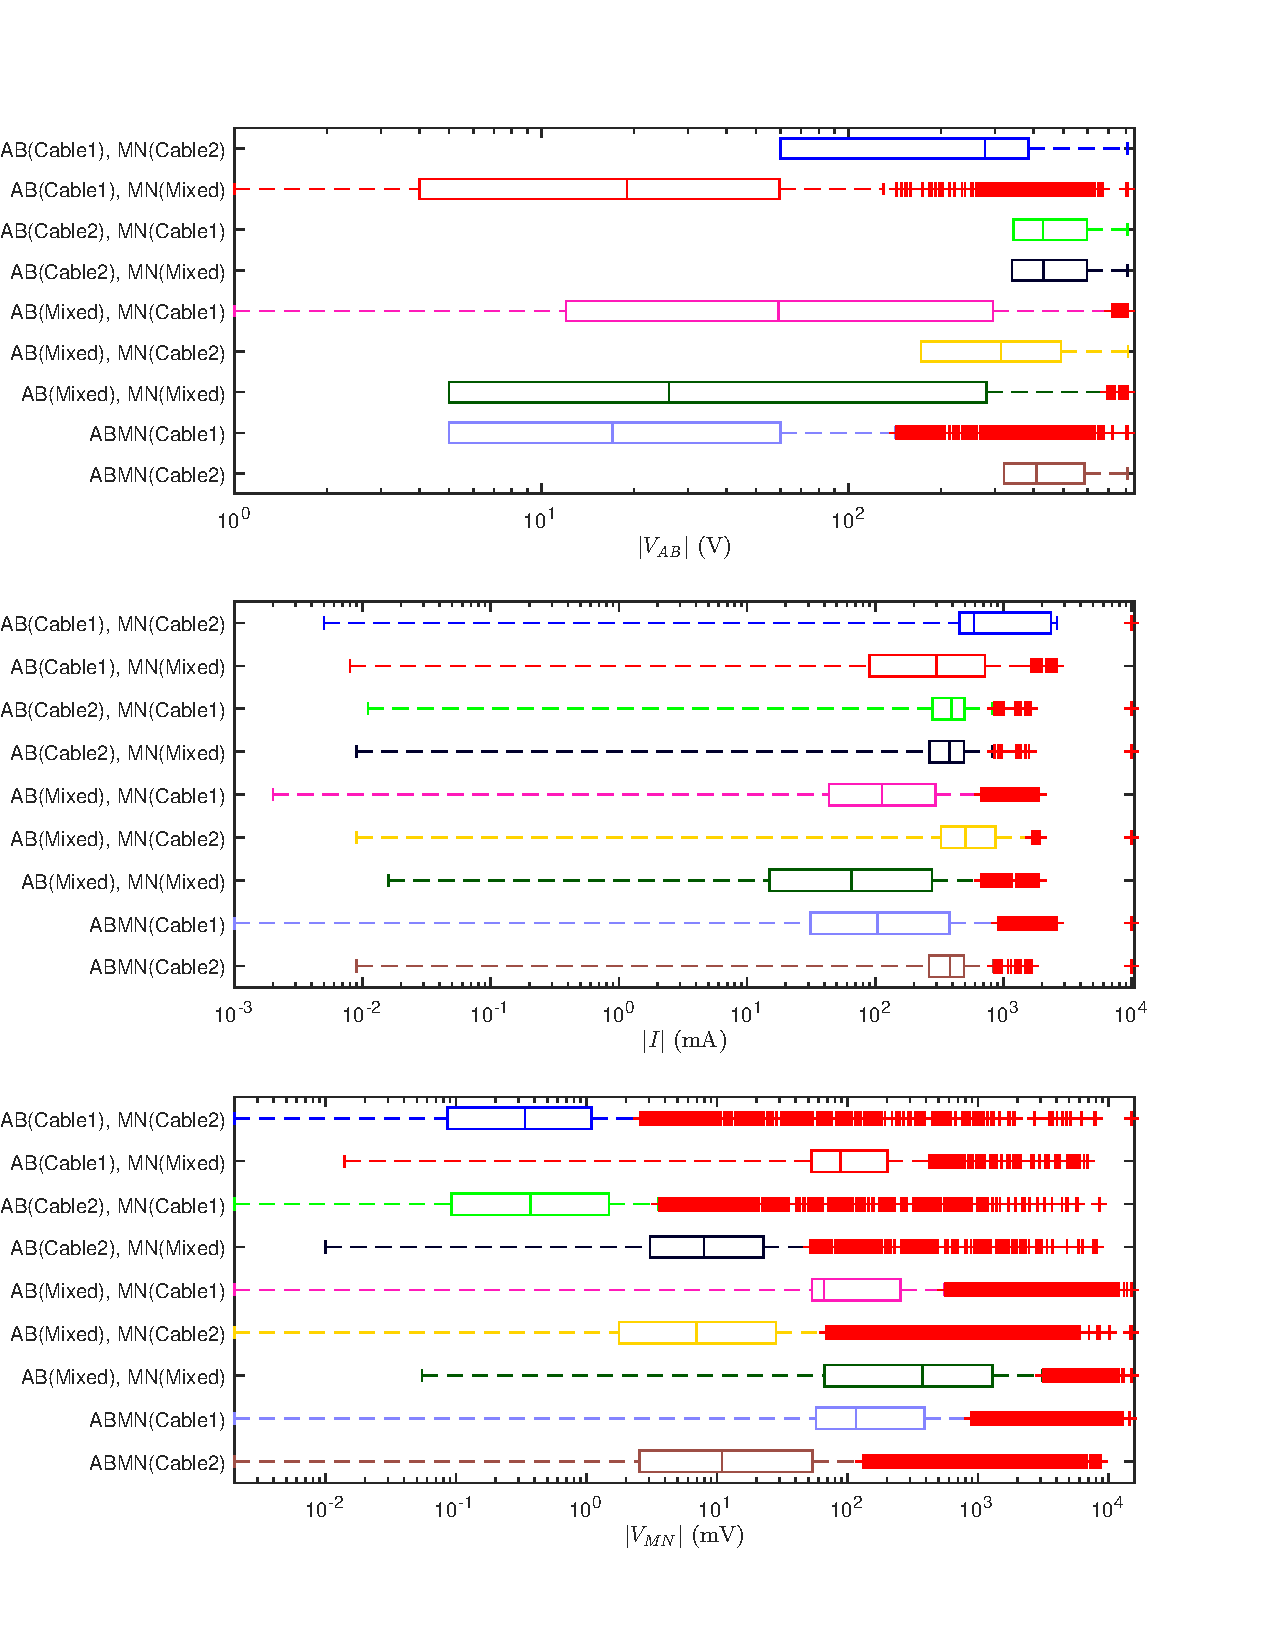
\includegraphics[trim=0cm 1.5cm 2cm 2cm, clip=true,width=0.86\linewidth]{./Figures/Fig9a.pdf}
       } \\%
    \subfigure{%
       \label{fig:CableSplit_Cluster_PropBoxPlot2}
    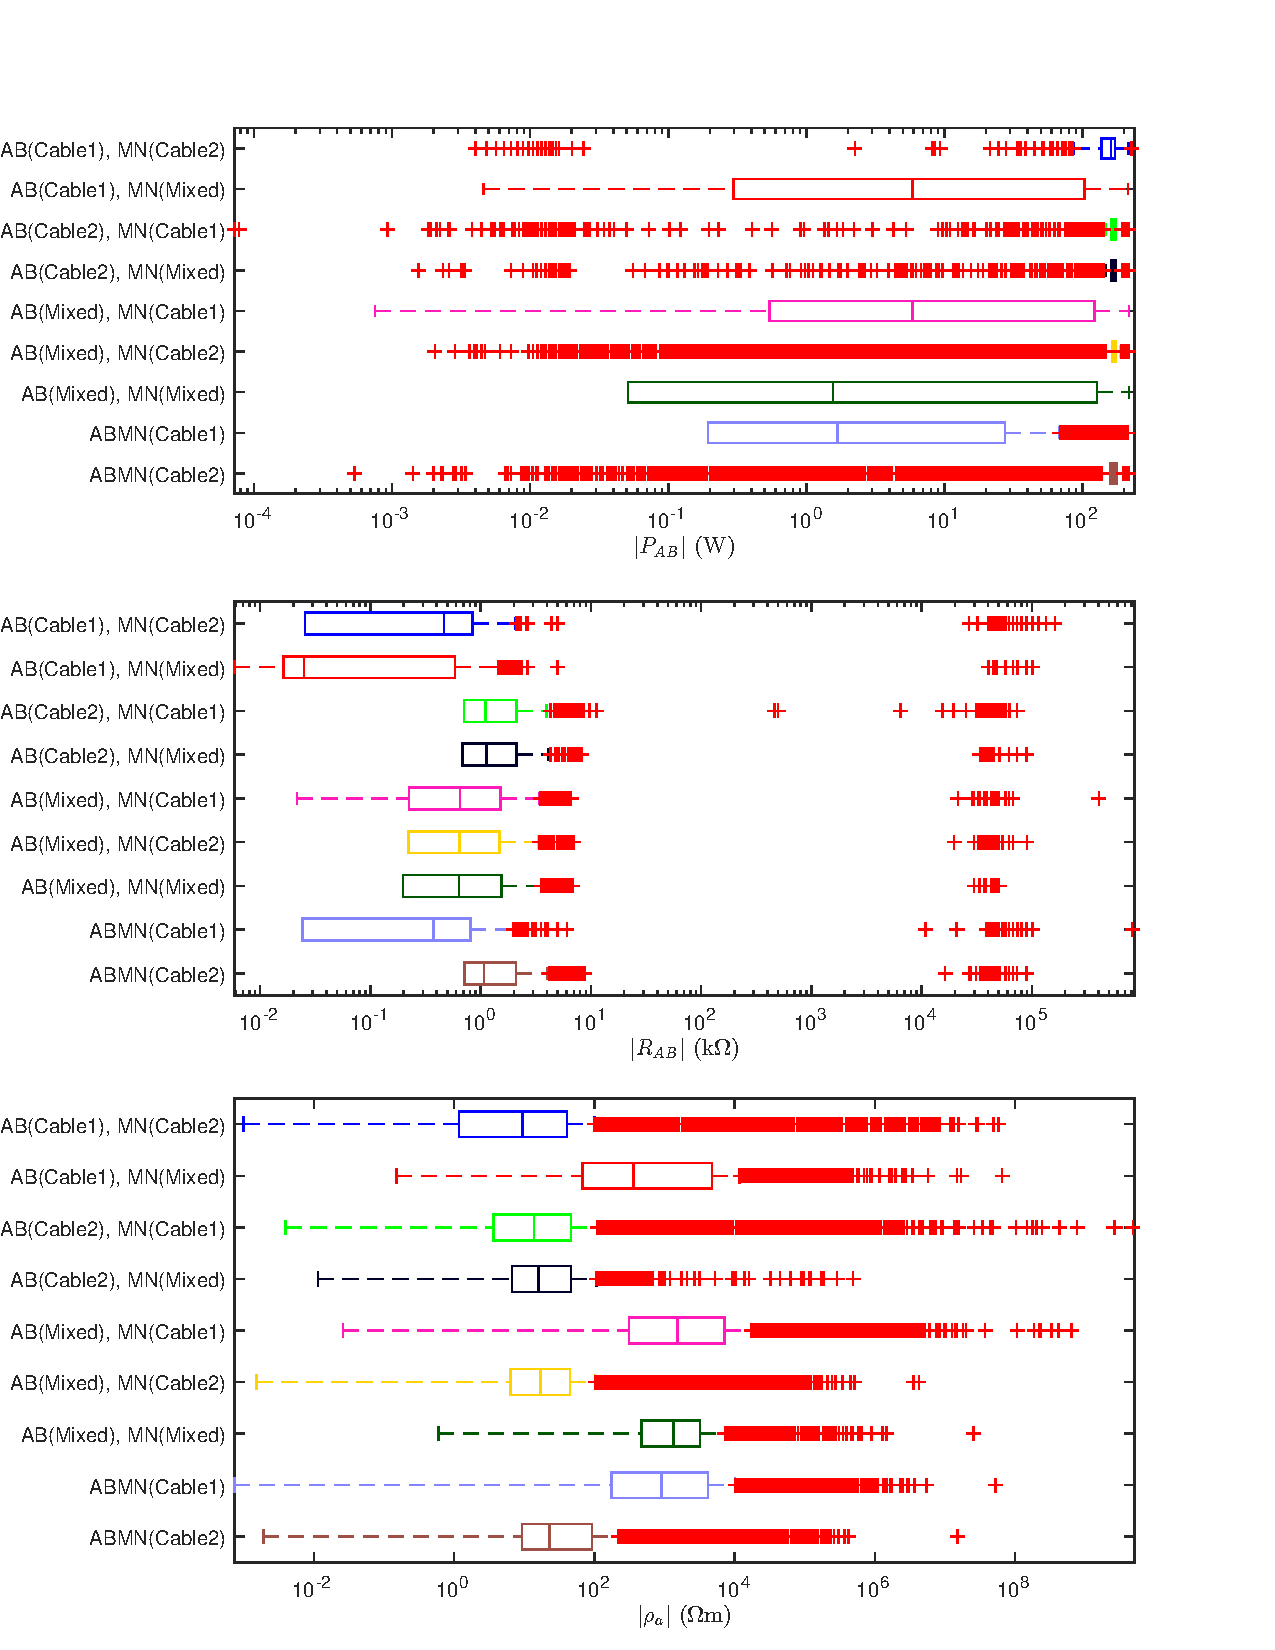
\includegraphics[trim=0cm 0.3cm 2cm 2cm, clip=true,width=0.86\linewidth]{./Figures/Fig9b.pdf}
       } %
    \end{center}
\caption{A series of boxplots which show the distribution of various data parameters in each of the cable based subsets. From these distributions it is possible to roughly characterize the signature of those data which are most contaminated by current leakages.}
\label{fig:CableSplit_Cluster_PropBoxPlots}
\end{figure}

As shown in Figure \ref{fig:CableSplit_Cluster_PropBoxPlots} those data which appear most contaminated by current leakages are characterized by:
\begin{itemize}
	\item{low TX voltage ($V_{AB}$)}
	\item{low injection current ($I$)}
	\item{high potential difference ($V_{MN}$)}
	\item{low TX power ($P_{AB}$)}
	\item{slightly low TX resistances ($R_{AB}$)}
	\item{high apparent resistivity ($\rho_{a}$)}
\end{itemize}
Current leakages can produce elevated $V_{MN}$ measurements since any type of deficiency in the cable insulation or electrical shorts between pins in the connection boxes can cause other electrodes to behave like additional sources (both current sources and current sinks). If these unaccounted for sources are closer to the M and N potential electrodes than the A or B current electrodes it can produce a sizable increase in measured potential differences. 

The low $P_{AB}$, $V_{AB}$, and $I$ associated with many of the measurements are directly linked to the high $V_{MN}$ measurements since the Syscal Pro modulates the TX voltage ($V_{AB}$), and therefore the TX power, $P_{AB} = V_{AB} I$, to maintain a ``constant'' measured potential difference between the M and N electrodes ($V_{MN}$) of 50 mV. If the test $V_{MN}$ measurements are too large then $V_{AB}$ is decreased which also decreases the injection current ($I$) since the resistance ($R_{AB}$) of the earth and instrument system is fixed for a particular TX (Ohm's Law: $V_{AB}$ = $I$ $R_{AB}$). Decreasing both $V_{AB}$ and $I$ decreases the TX power ($P_{AB} = I V_{AB}$). The elevated $\rho_{a}$ values are also a result of the high $V_{MN}$ and low $I$ measurements as shown by the following equation,  
\begin{equation}
 \rho_{a} \approx \frac{V_{MN}}{I} 4 \pi \left[ \frac{1}{\overline{AM}} - \frac{1}{\overline{BM}} - \frac{1}{\overline{AN}} + \frac{1}{\overline{BN}} \right]^{-1} = \frac{V_{MN}}{IG}
\end{equation}    
where $G$ is the geometric factor.

From this analysis it is possible to determine which of the cable based subsets are the most contaminated by current leakages. Further analysis can then be focused on the less contaminated subsets with the hope of isolating noisy measurements to create a reliable data subset for inversion and interpretation. Those cable based subsets which warrant further analysis include: (1) AB-Cable1, MN-Cable2, (2) AB-Cable2, MN-Cable1, (3) ABMN-Cable2, and (4) AB-Mixed, MN-Cable2.

By looking at the least contaminated data, those in which the TX and RX electrodes are on separate cables, troublesome electrodes such as electrodes 15 and 113 are easy to identify due to their comparatively high median misfits (see plots \ref{fig:Boxplot_AB_Cable1_MN_Cable2_Misfit_vs_M_ElecID} and \ref{fig:Boxplot_AB_Cable2_MN_Cable1_Misfit_vs_M_ElecID}). These troublesome electrodes are not as easy to identify using SVD analysis on the cable based subsets. While the first few singular vectors from the high misfit data show peaks at electrode 15 and 113 there are a number of other peaks which complicate the interpretation. 

Further analyzing the distribution of measured survey parameters using boxplots, similar to those in Figure \ref{fig:CableSplit_Cluster_PropBoxPlots}, it is possible to make basic deductions regarding the source of contaminating noise for each troublesome electrode. Table \ref{tab:BadElec_Props}, summarizes the differences in observed parameters for the two troublesome electrodes. Electrode 113 appears to have a very high contact resistance which makes it difficult to push a sizable current, when the electrode is used as an A or B current electrode. This results in a low transmitter power and low $V_{MN}$ potential differences. Identifying the source of noise impacting those data which incorporate electrode 15 is not as simple. Although it is possible that electrode 15 is one of the primary sources of the current leakages it is hard to prove this since there is not a strong correlation between high misfit data and those data with at least one electrode in close proximity to electrode 15. Due to the clearly inconsistent nature of data associated with electrodes 15 and 113 we removed these data from the inversion dataset. Although electrode 40 also has a comparatively high median misfit when it is used as an M electrode in the full dataset (Figure \ref{fig:Boxplot_Full_DataMisfit_vs_MElecID}) it is not correlated with high normalized misfits in the less contaminated data subsets. This indicates that the observed correlation between electrode 40 and high normalized misfits in Figure \ref{fig:Boxplot_Full_DataMisfit_vs_MElecID} is likely due to the current leakages, or some factor other than the electrode itself.

\begin{table}[!ht]
\begin{center}
  \begin{tabular}{| c | c | c |}
    \hline
     & Electrode 15 &  Electrode 113 \\ \hline
    $V_{AB}$ & Moderate & Very High (maxed) \\ 
    $I$ & Low & Very Low \\
    $V_{MN}$ & High & Moderate \\
    Data Misfit & High & High \\
    $P_{AB}$ &  Low & Very Low \\
    $R_{AB}$ & Moderate & Very High \\
    $\rho_{a}$ & High & High \\
    \hline
  \end{tabular}
\caption{Relative differences between the survey parameters associated with the suspicious electrodes 15 and 113 when compared with the remainder of the data where the TX and RX electrodes are on separate cables.}
\label{tab:BadElec_Props}
\end{center}
\end{table} 

Identifying electrical noise from infrastructure may also be possible using this approach. If the contaminating noise is isolated to a specific electrode or group of electrodes in the same region they can be identified. Different types of infrastructure will undoubtedly bias measurements in different ways. Since the signature of infrastructure based noise may be difficult to theoretically characterize it is important to have detailed field notes which describe the location of all possible infrastructural noise sources. We do not believe that electrode 15 is impacted by infrastructural noise since it is located in a region with very little infrastructure.  

Through our manual search we have identified current leakages within the cables and/or connecting boxes as the primary source of electrical noise in our survey. Current leakages are more prevalent within Cable 1 than Cable 2, but both cables are affected. In addition to the current leakages 2 troublesome electrodes have been identified which are consistently associated with high misfit data. As a result of the magnitude and extent of the contamination some subsets of the data will simply be discarded while others warrant further analysis. For this we proceed into Stage II, where data clustering is utilized to identify and separate out highly contaminated data from the remaining data subsets to attain a reliable dataset for the final inversion and interpretation. 

\subsection{Stage II: Cluster Analysis}
\label{Data_Quality_Control:StageII_Cluster_Analysis}

Although we have identified several sources of noise and removed some of the most heavily contaminated data the remaining data subsets still require extensive data QC analysis to help remove lingering effects of the current leakages and possibly other secondary noise sources. Accurately identifying and dealing with these contaminated data is a challenging problem since the characteristic patterns may be obscured by the presence of pattern overprinting from multiple noise sources. 

\begin{figure} [!ht]
\begin{center}
   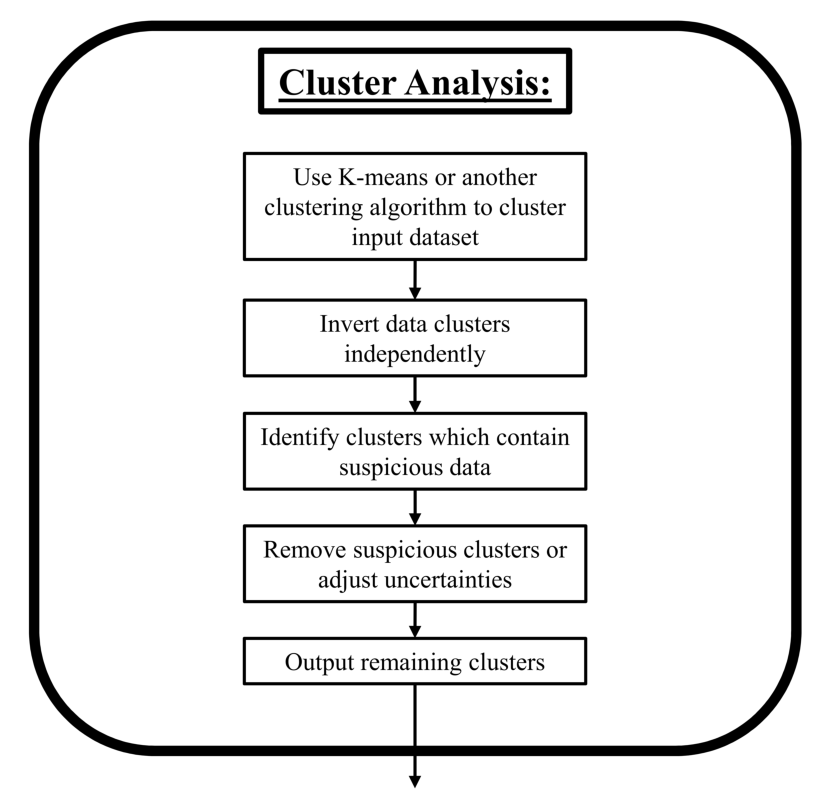
\includegraphics[trim=0cm 0cm 0cm 0cm, clip=true,width=0.75\linewidth]{./Figures/Fig10.pdf}    
\end{center}
\caption{General cluster analysis workflow.}
\label{fig:DataQC_workflow_ClusterAnalysis}
\end{figure}

To remove some of the subjectivity from the search for correlations between survey parameters and high misfit data, cluster analysis as detailed in Figure \ref{fig:DataQC_workflow_ClusterAnalysis} is employed. Our cluster analysis is based on the $k$-Means data clustering algorithm \citep{MacQueen1967}. Based on the parameters provided for each data point, the $k$-Means algorithm partitions the data into a predefined number of clusters. To start, each cluster is randomly assigned a data point. New points are then iteratively added to the cluster with the nearest centroid, and the cluster means are recomputed to account for the additional points. This iterative process continues until there are no reassignments of data to different clusters or the decrease in the squared error is small. \cite{Jain1999} provide a good review of $k$-Means data clustering as well as other clustering algorithms. A complete outline of Stage II shown in Figure \ref{fig:DataQC_workflow_StageII}.

\begin{figure} [!ht]
\begin{center}
   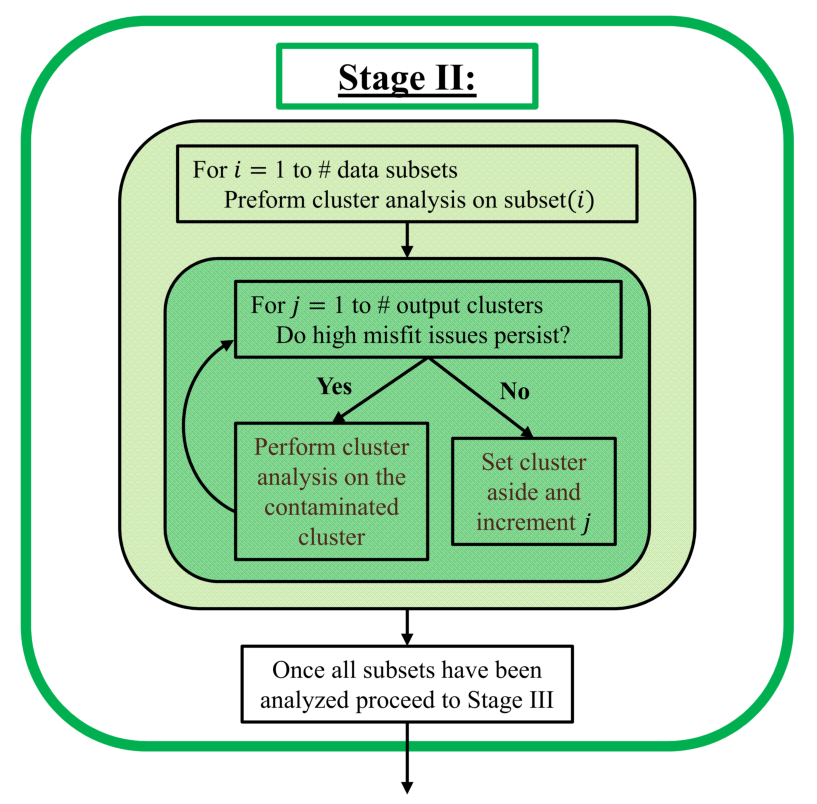
\includegraphics[trim=0cm 0cm 0cm 0cm, clip=true,width=0.75\linewidth]{./Figures/Fig11.pdf}     
\end{center}
\caption{Detailed workflow for Stage II.}
\label{fig:DataQC_workflow_StageII}
\end{figure}

The first step is to decide which data parameters to use in the clustering. After multiple trials, a simple clustering based on $V_{MN}$, $V_{AB}$, $I$, and the normalized data misfit from the inversion iteration where $\phi_d$ begins to plateau was chosen. Depending on the application and type of noise present, other parameters may also prove useful for clustering. Before clustering, the data need to be normalized so that each of the parameters are on the same general scale. Since the distribution of parameters is not normally distributed, the following normalizations were tested: z-score normalization and dividing by the $l_{2}$ or $l_{1}$ norm of the data. Although the observed differences in the resulting clustering were very small the $l_{2}$ normalization was chosen since the clusters appeared to be slightly tighter. 

Choosing the optimal number of clusters is a topic of interest in machine learning. One approach for determining the number of clusters is the L-curve method. In this method the number of clusters is determined by the corner point in a plot of a cluster evaluation metric versus the number of clusters specified \citep{Salvador2004}. Trials were run with 2-12 clusters on multiple subsets of the data and the Akaike and Bayesian information criterions (AIC and BIC respectively) were computed for each clustering. These criterion provide a general measure of how well the data are clustered while enforcing a penalty for each additional cluster. Plots of these information criterions versus the number of clusters suggest that the corner point typically falls between 4-6 clusters. For the sake of efficiency all subsequent clustering analysis was done using 6 clusters. Although not all of the tested subsets required 6 clusters to characterize the data, for this application it is better to have 1-2 extra clusters than too few.  

\begin{figure} [!ht]
    \begin{center}  
    \subfigure[]{%
       \label{fig:AB_Mixed_MN_Cable2_Vmn_vs_I_Cluster}
       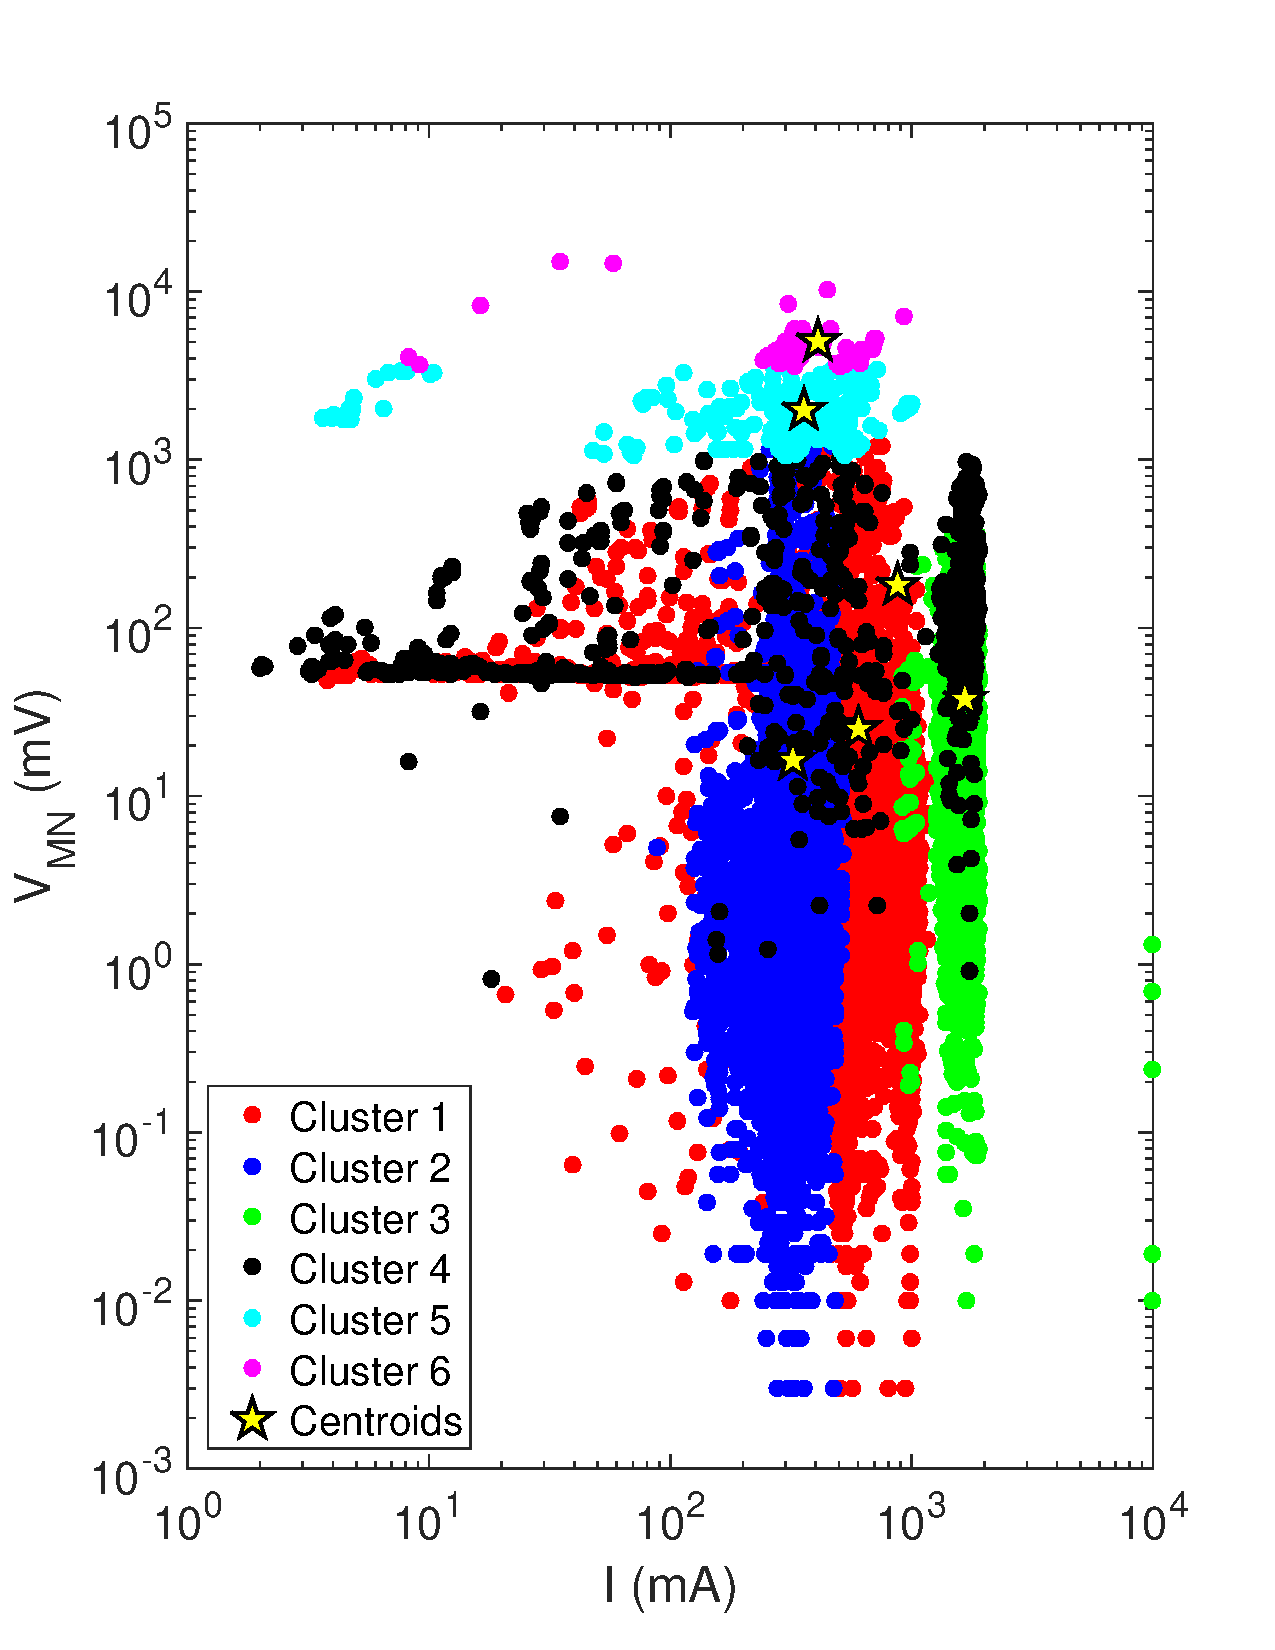
\includegraphics[trim=0.3cm 0.7cm 1.5cm 1.8cm, clip=true,width=0.475\linewidth]{./Figures/Fig12a.pdf}
       } %      
    \subfigure[]{%
       \label{fig:AB_Mixed_MN_Cable2_Vab_vs_I_Cluster}
       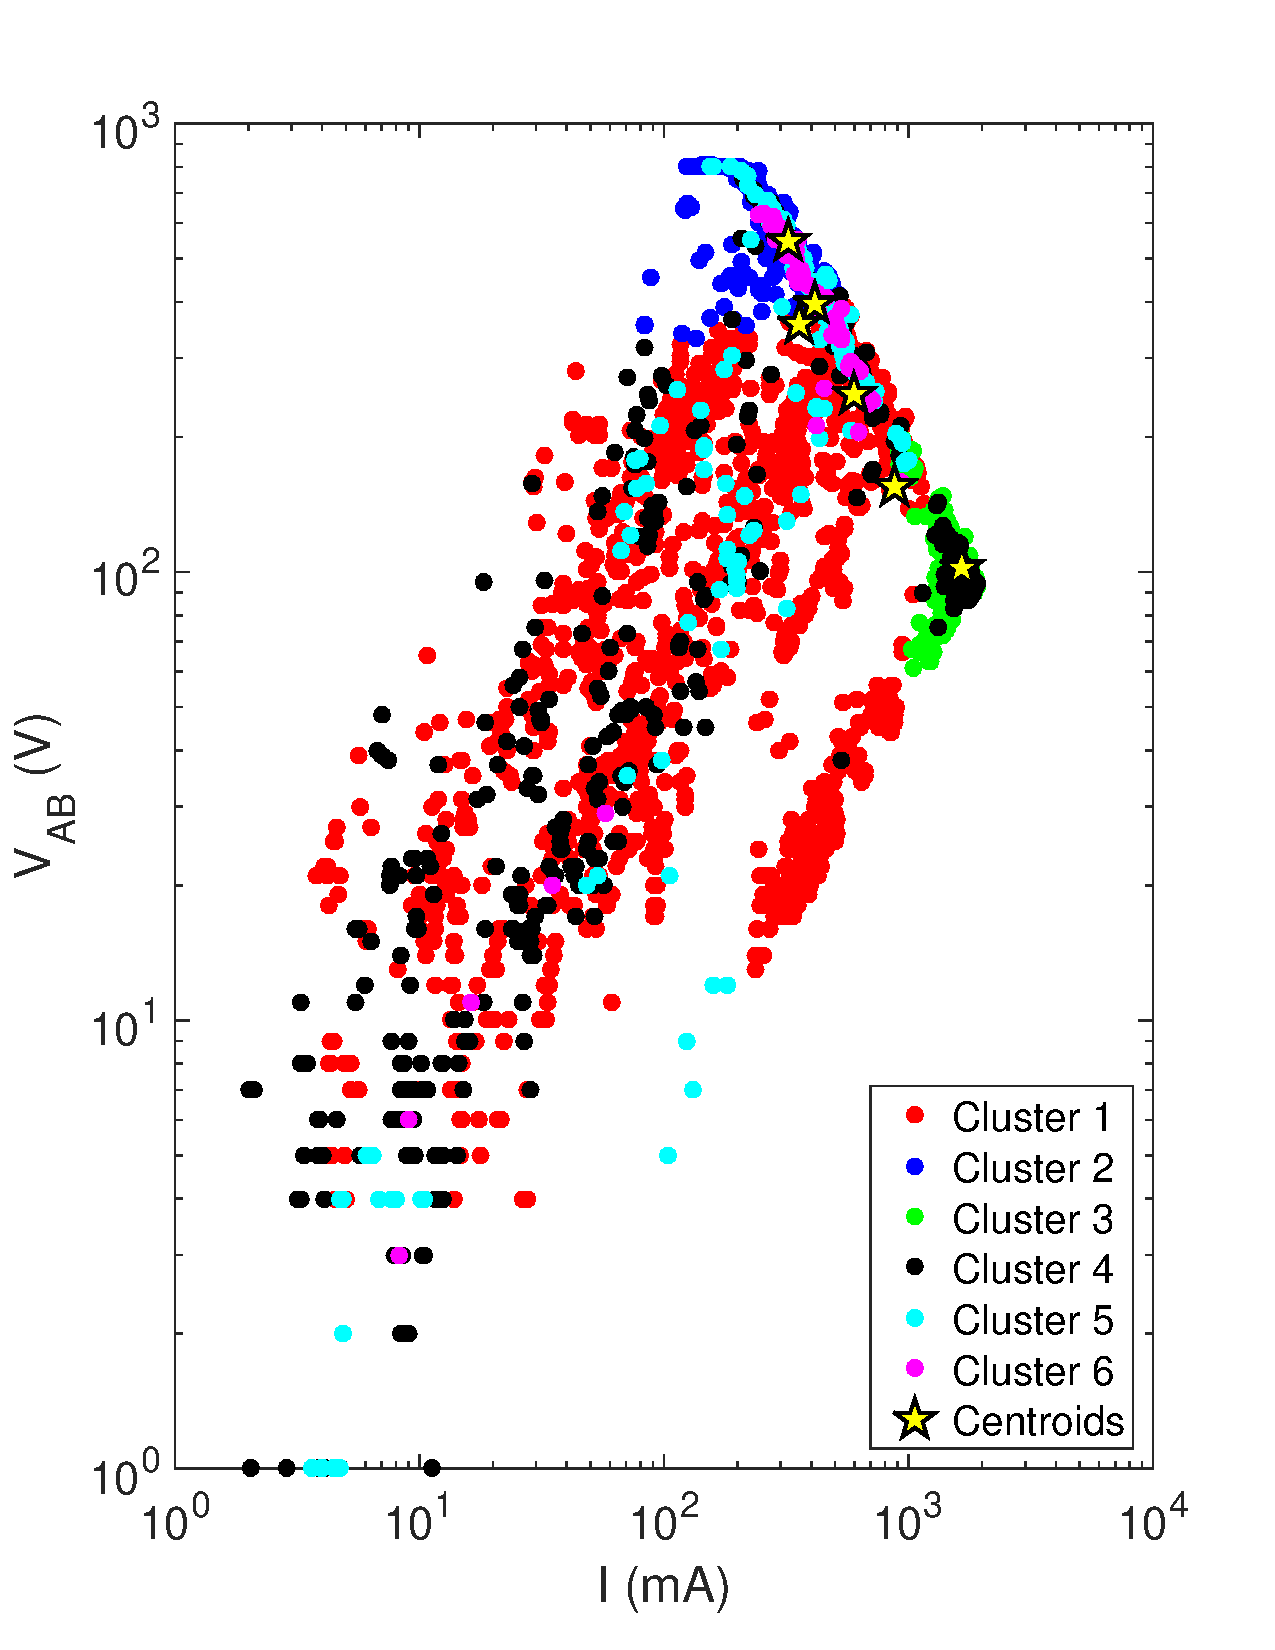
\includegraphics[trim=0.3cm 0.7cm 1.5cm 1.8cm, clip=true,width=0.475\linewidth]{./Figures/Fig12b.pdf}
       } %   
    \end{center}
\caption{Plots showing the distribution of data clustering results, from the AB-Mixed, MN-Cable2 subset, in two different variable spaces. Analyzing the visual distribution of the clusters can be useful for identifying patterns and characterizing clusters which contain suspicious data.}
\label{fig:AB_Mixed_MN_Cable2_ClusterComp}
\end{figure}

\begin{figure} [!ht]
    \begin{center}
    \subfigure{%
       \label{fig:AB_Mixed_MN_Cable2_Cluster_PropBoxPlot1}
       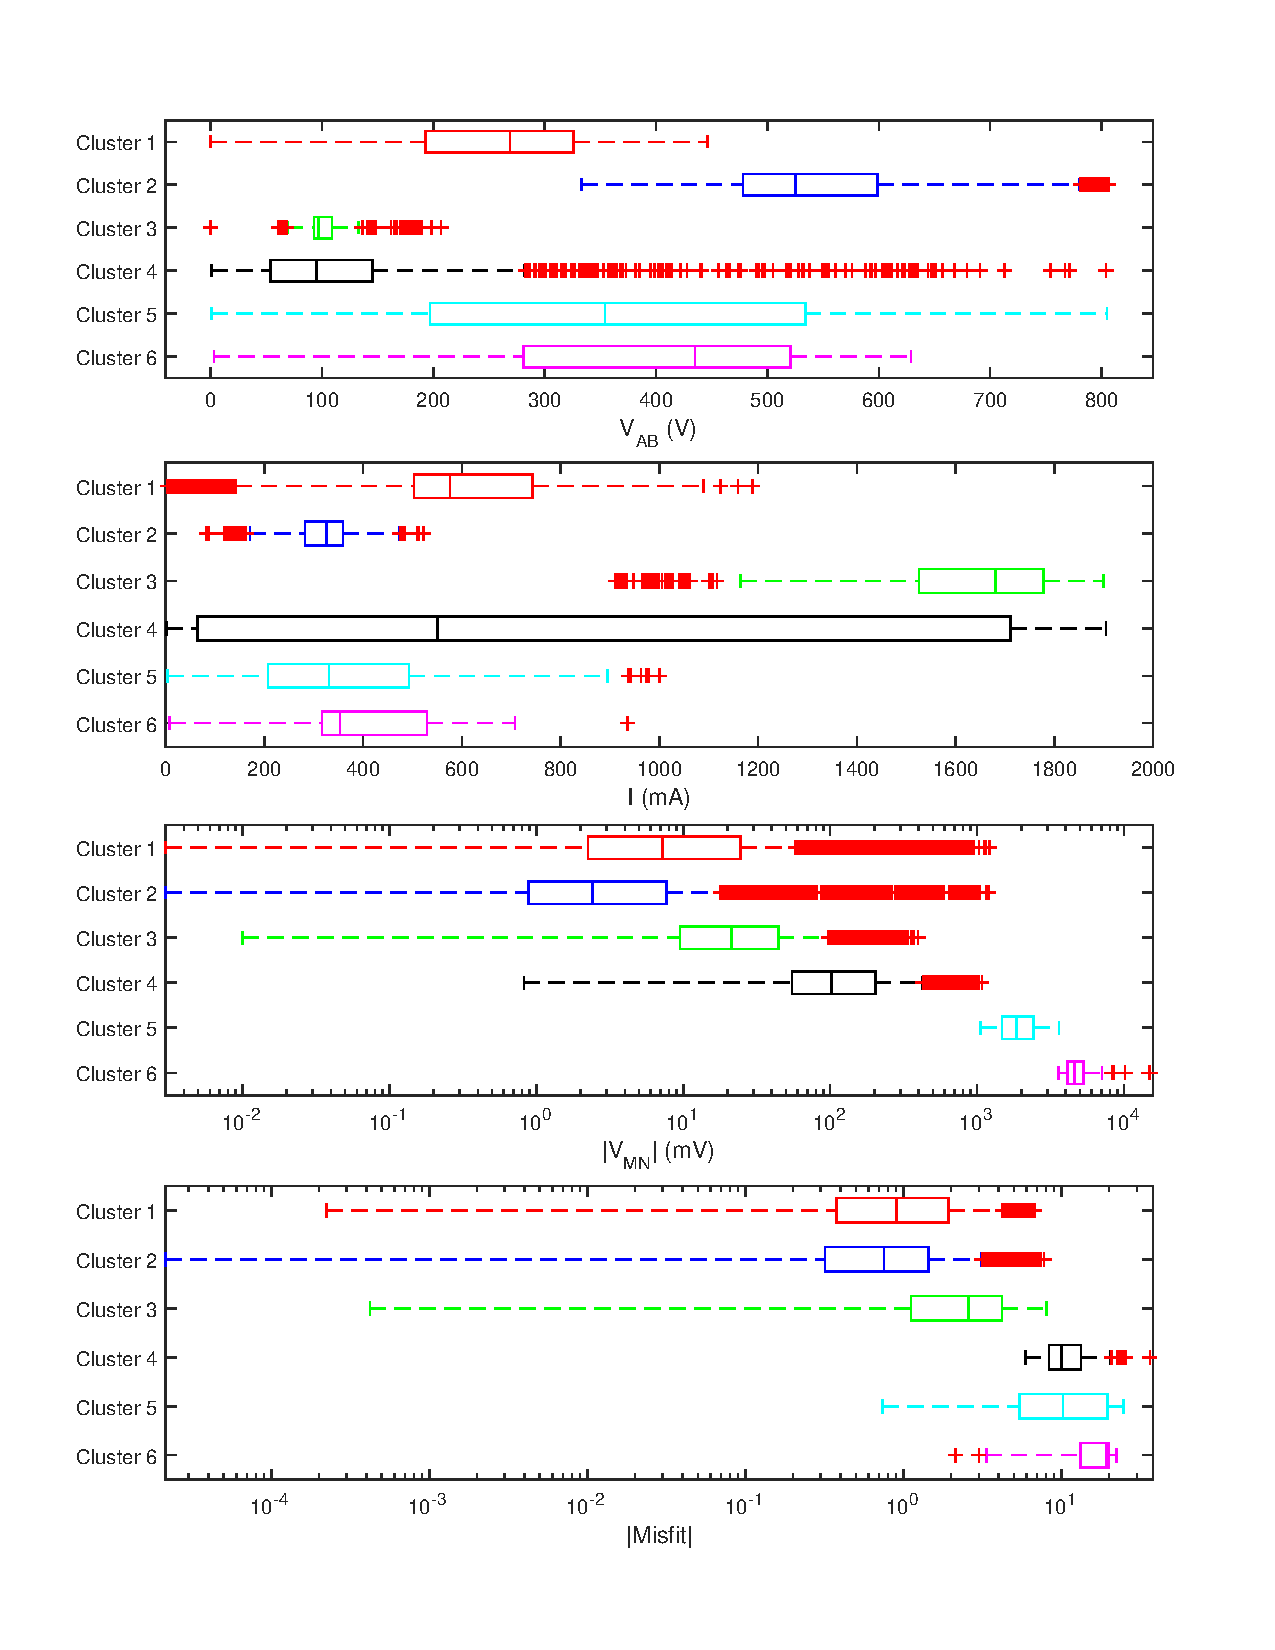
\includegraphics[trim=1cm 1.5cm 2cm 2cm, clip=true,width=0.86\linewidth]{./Figures/Fig13a.pdf}
       } \\%
    \subfigure{%
       \label{fig:AB_Mixed_MN_Cable2_Cluster_PropBoxPlot2}
    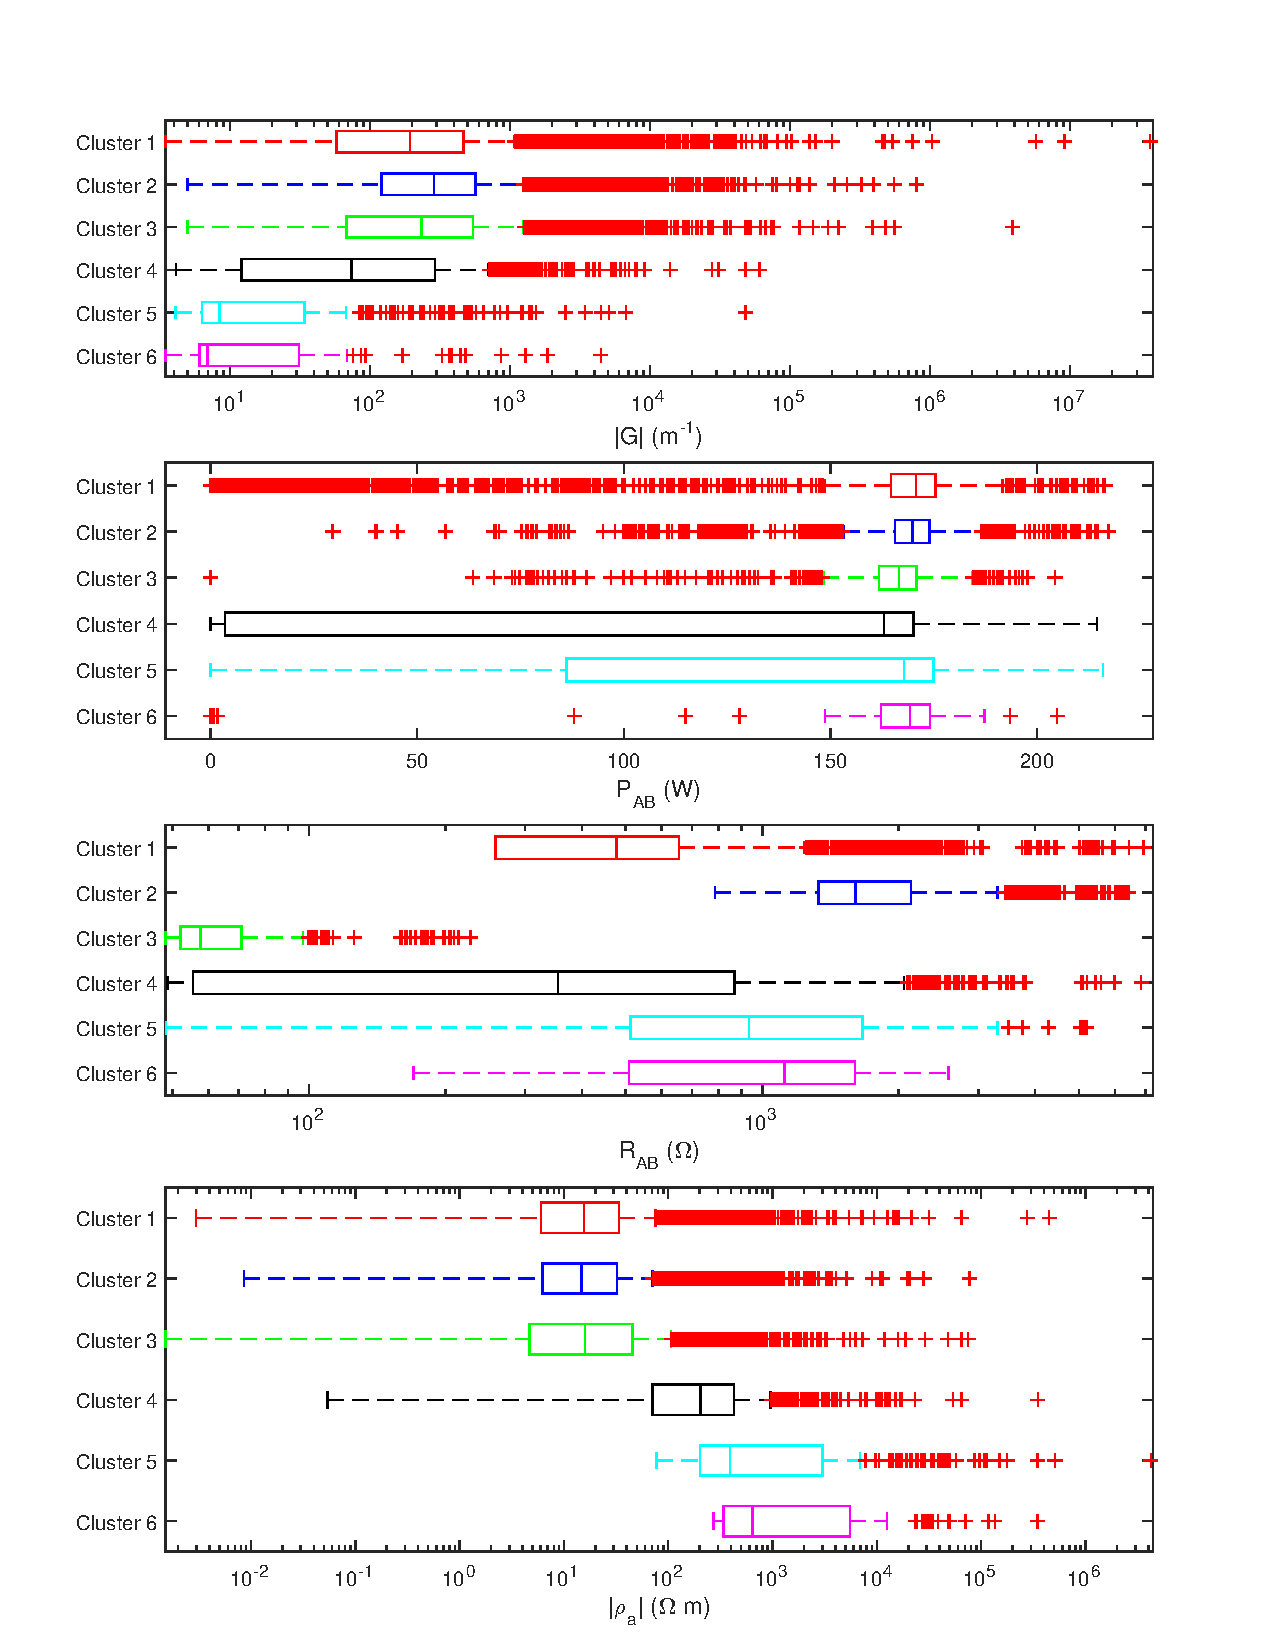
\includegraphics[trim=1cm 0.5cm 2cm 2cm, clip=true,width=0.86\linewidth]{./Figures/Fig13b.pdf}
       } %
    \end{center}
\caption{Boxplots showing the distribution of survey parameters in each cluster from the the AB-Mixed, MN-Cable2 subset. High normalized misfits and the characteristic signatures of noise sources identified in Stage I allow us to identify contaminated clusters.}
\label{fig:AB_Mixed_MN_Cable2_Cluster_PropBoxPlots}
\end{figure}

An example of the data clustering is presented here using the AB-Mixed, MN-Cable2 data subset. Figure \ref{fig:AB_Mixed_MN_Cable2_ClusterComp} shows the distribution of the clusters in different parameter spaces. Boxplots showing the distribution of survey parameters associated with each cluster are shown in Figure \ref{fig:AB_Mixed_MN_Cable2_Cluster_PropBoxPlots}. Together these plots allow us to identify clusters containing inconsistent or highly noise-contaminated data, and search for correlations which provide clues as to the source of the contaminating noise. The boxplots show that clusters 4-6 have many of the traits which characterized the data which were highly contaminated by current leakages in Stage I (i.e. high $V_{MN}$, high $\rho_a$, high normalized data misfits, and lower $P_{AB}$).

After clustering the data, each of the clusters are then inverted independently. If the inversion of an individual cluster converges easily to the target misfit then the data within that cluster is deemed self-consistent and the cluster is set aside for recombination in Stage III. For clusters with moderately large normalized misfits we iterate the data clustering process by further clustering the data within that cluster. In this way we are further subdividing the data to look at clusters of clusters. Through this process a tree of clusters is created (see Figure \ref{fig:ClusterTree}). Clusters, such as clusters 4-6 from the AB-Mixed, MN-Cable2 data subset shown above, with very high normalized misfits, are deemed to be inconsistent and are either discarded or their uncertainties are adjusted. Boxplots like those in Figure \ref{fig:AB_Mixed_MN_Cable2_Cluster_PropBoxPlots} are used to visualize the distribution of parameters within each cluster and identify the signature of possible noise sources. This process continues until all of the clusters associated with a particular data subset have been analyzed. 

\begin{figure} [h!]
\begin{center}
   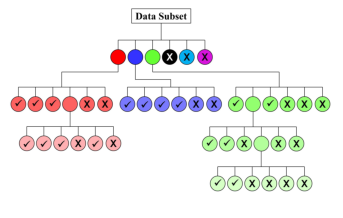
\includegraphics[trim=0cm 0cm 0cm 0cm, clip=true,width=0.75\linewidth]{./Figures/Fig14.pdf}     
\end{center}
\caption{Hypothetical cluster tree diagram showing the verified clusters with a check and the discarded clusters with a X. Each color denotes a cluster and its possible sub-clusters.}
\label{fig:ClusterTree}
\end{figure} 

By breaking the data up into subsets and then clustering the subsets we increase the number of inversions which need to be run in order to verify the self-consistency of the data in each of these groupings. However, each of these inversions becomes a smaller problem to solve. This process is easily parallelized, since each cluster and each subset is analyzed independently at this stage. 

It is important to stress that at this stage we are only checking the self-consistency of data in each cluster. There is a danger that inversions of small clusters may be able to easily fit the data due to a lack of data to constrain various parts of the model space. However, any contaminated or inconsistent data which slip through Stage II in this manner will be caught and dealt with in the following stages as we build the dataset back up and check for inter-cluster and inter-subset consistency. Once all of the data subsets which passed Stage I, have completed Stage II we proceed to Stage III.

\subsection{Stage III: Recombine Verified Clusters From Each Subset}
\label{Data_Quality_Control:StageIII_Recombine_Clusters}

\begin{figure} [!ht]
\begin{center}
   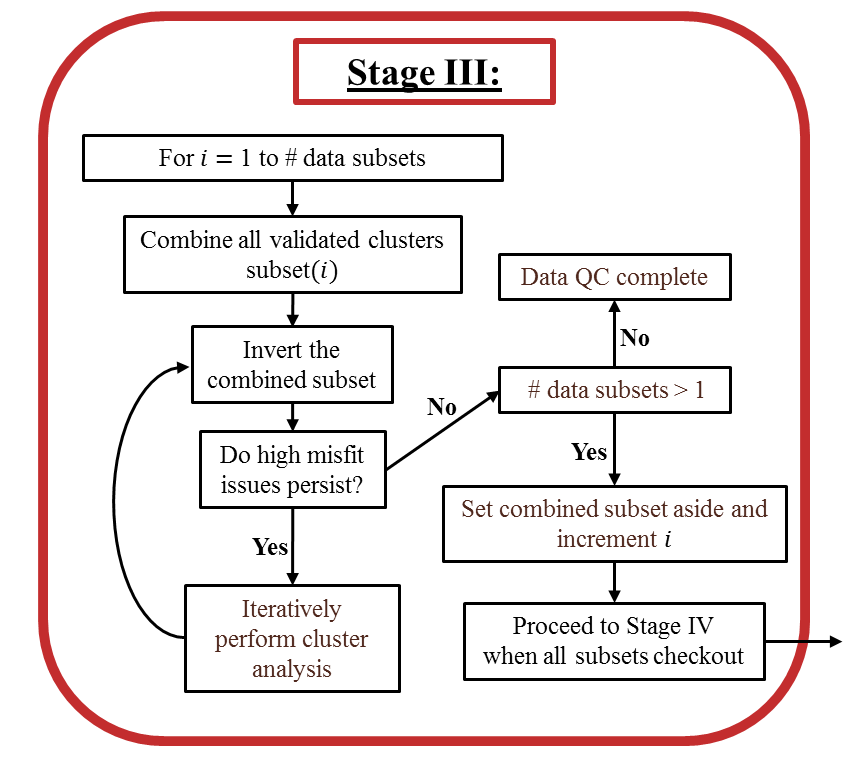
\includegraphics[trim=0cm 0cm 0cm 0cm, clip=true,width=0.8\linewidth]{./Figures/Fig15.pdf}     
\end{center}
\caption{Detailed workflow for Stage III.}
\label{fig:DataQC_workflow_StageIII}
\end{figure}

In Stage III all of those clusters from a given subset, which were verified in Stage II (i.e. checked clusters in Figure \ref{fig:ClusterTree}) are recombined and then re-inverted (see Figure \ref{fig:DataQC_workflow_StageIII} for an outline). If high misfit issues persist then cluster analysis is iteratively performed on the recombined subset until any inter-cluster inconsistencies (i.e. data which may have been consistent with other data in their cluster, but are not consistent with data in other clusters) are dealt with. Since most of the contaminated data has been dealt with in the first two stages this second round of cluster analysis should proceed quickly. By putting each subset through this recombining process separately we keep the size of the datasets small so that the analysis and inversions can be completed quickly. Comparing the recovered inversion models from each data subset can be useful since it provides insight into how well different portions of the model are constrained by the data in each subset.   

If only one subset of data came out of Stage I then the data quality control process is completed here in Stage III and the recombined subset should contain reliable data from which a final inversion model can be obtained. If multiple subsets of data came out of Stage I then proceed to Stage IV where the consistent subsets are recombined into a single dataset. 

Table \ref{tab:DataSubsetSizes} shows the sizes of the data subsets, which were selected for further analysis in Stage I, both before any data were removed and after Stage III of the data QC process was completed. From this table it is evident that each subset was affected by the current leakages and other possible noise sources to different degrees.

\begin{table}[!ht]
\scriptsize
\begin{center}
  \begin{tabular}{| c | c | c | c |}
    \hline
    \bf{Data Subset} & \bf{\# Data (Pre-QC)} & \bf{\# Data (Post-QC)} & \bf{\% Discarded} \\
    \hline
    AB-Cable1, MN-Cable2 & 8,183 & 6,335 & $22.6 \%$ \\
    \hline
    AB-Cable2, MN-Cable1 & 9,485 & 7,584 & $20.0 \%$\\
    \hline
    ABMN-Cable2 & 10,997 & 6,775 & $38.4 \%$\\
    \hline
    AB-Mixed, MN-Cable2  & 22,134 & 4,703 & $78.8 \%$\\
    \hline
    Full Dataset  & 95,194 & 25,397 & $73.3 \%$\\
    \hline    
  \end{tabular}
\caption{Data subset sizes}
\label{tab:DataSubsetSizes}
\end{center}
\end{table}

\subsection{Stage IV: Recombine Verified Subsets}
\label{Data_Quality_Control:StageIV_Recombine_Subsets}

\begin{figure} [!ht]
\begin{center}
   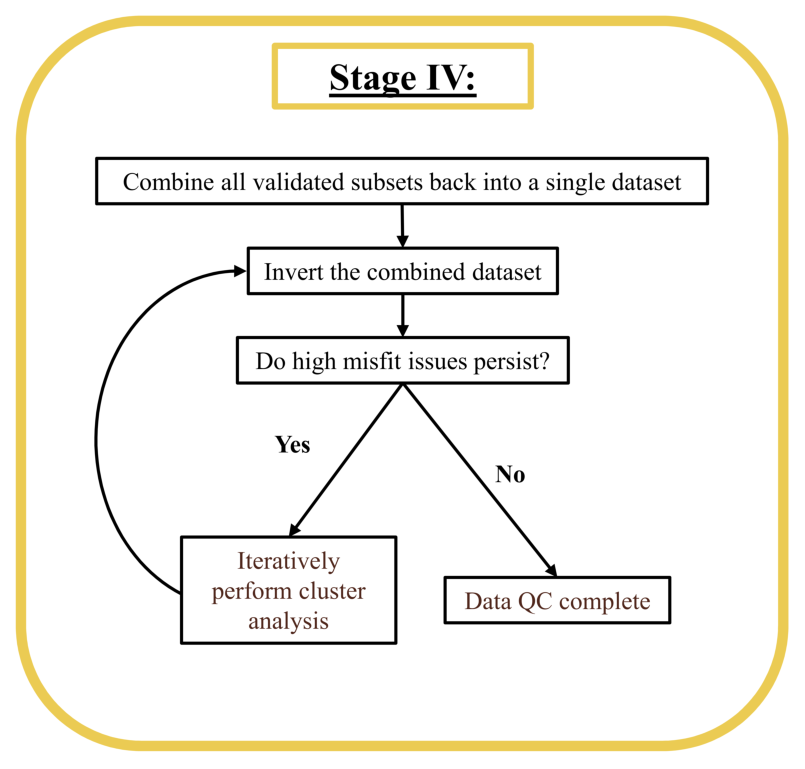
\includegraphics[trim=0cm 0cm 0cm 0cm, clip=true,width=0.75\linewidth]{./Figures/Fig16.pdf}     
\end{center}
\caption{Detailed workflow for Stage IV.}
\label{fig:DataQC_workflow_StageIV}
\end{figure}

In this final stage of the data QC process we recombine the various subsets, which where checked in Stage III, to form a single dataset which can be inverted to obtain a final inversion model. Figure \ref{fig:DataQC_workflow_StageIV} shows an outline of this process. First, all of the data subsets are combined and re-inverted. If the inversion algorithm struggles to adequately fit the data then a final round of cluster analysis is warranted. As in Stage III the cluster analysis is iteratively applied to the recombined dataset. Since the self-consistency of each subset was verified in Stage III, we are now trying to identify inter-subset inconsistencies. For the Mosaic field dataset presented here, additional cluster analysis was not necessary at this stage. However, depending on the dataset and the noise sources present, some troublesome data may remain. These inconsistent clusters may need to be thrown out, or their uncertainties may need to be adjusted. The final line of Table \ref{tab:DataSubsetSizes} compares the original size of the full dataset with that of the final dataset from the data QC process. Due to the highly contaminated nature of this dataset only $27\%$ of the data were retained.     

Through this data QC process, we are able to identify and deal with noise-contaminated data to produce a reduced dataset that contains only those data which have proven themselves to be consistent and reliable. By working with the various subsets of the data we have also had the chance to refine our assigned uncertainties to better balance the data misfit among clusters or subsets with different noise levels. Using this dataset and our refined uncertainty estimates, it is now possible to begin the formal inversion process to attain a conductivity model that can be interpreted with a higher degree of confidence.   


\section{Case Study Results}
\label{Case_Study_Results}

When you compare the inversion results from the full dataset (Figure \ref{fig:CaseStudy_InvMod_Full}) with the inversion model obtained after the data quality control process (Figure \ref{fig:CaseStudy_InvMod_Final}) there are large scale similarities. However, it is easier to interpret the post-QC model. In the initial inversion, most of the anomalies in the central region bleed together to form a generally more conductive region and it is difficult to identify individual anomalies. In the post-QC model there are 6 notable conductive anomalies which have been labeled as A-F in Figure \ref{fig:CaseStudy_InvMod_Final}. The location of many of these anomalies correlate well with those regions where moisture was observed in the mine. Since the post-QC model does a much better job of fitting the observed data (see Figure \ref{fig:CaseStudy_Inv_MisfitPlots}) it can be interpreted with a higher degree of confidence. 

\begin{figure} [!ht]
    \begin{center}
    \subfigure[Initial Model]{%
       \label{fig:CaseStudy_InvMod_Full}
       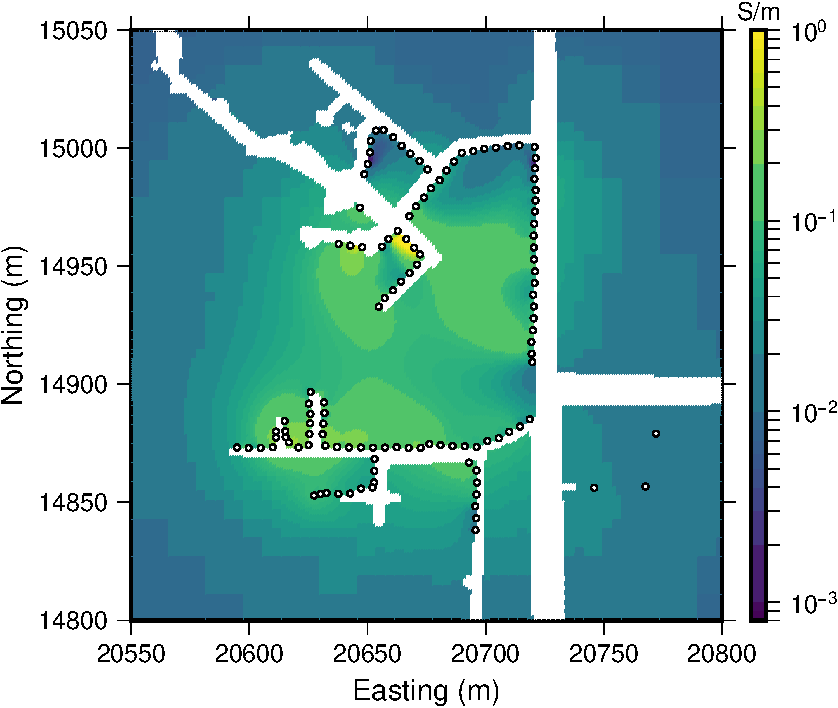
\includegraphics[trim=0cm 0cm 0cm 0cm, clip=true,width=0.95\linewidth]{./Figures/Fig17a.pdf}
       } \\%
    \subfigure[post-QC Model]{%
       \label{fig:CaseStudy_InvMod_Final}
       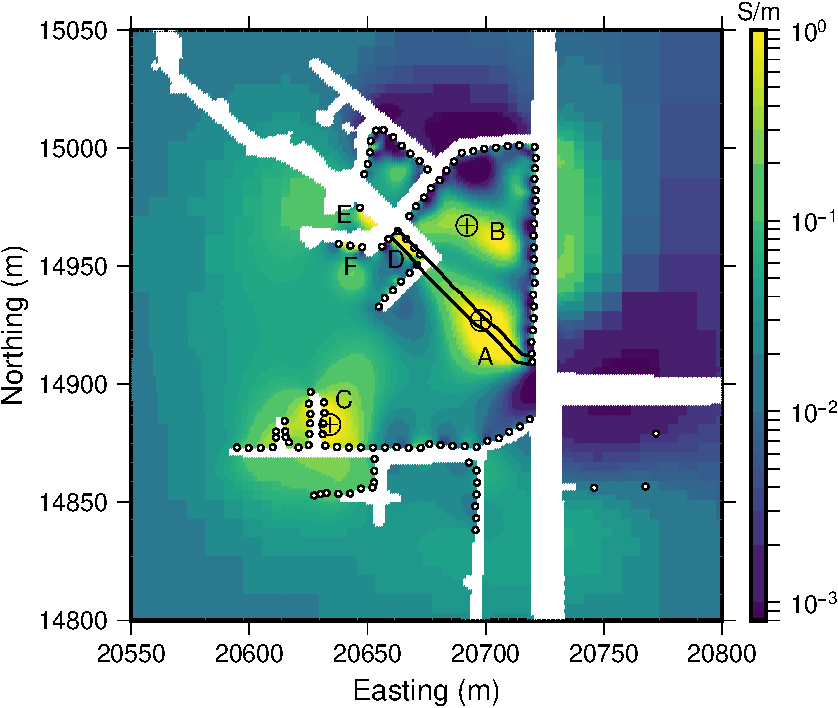
\includegraphics[trim=0cm 0cm 0cm 0cm, clip=true,width=0.95\linewidth]{./Figures/Fig17b.pdf}
       } %     
    \end{center}
\caption{Depth sections from the initial inversion model (panel \ref{fig:CaseStudy_InvMod_Full}) where the full dataset was used, and the  post-QC inversion model (panel \ref{fig:CaseStudy_InvMod_Final}). While many of the conductive anomalies in the initial inversion model bleed together to form a large diffuse region of high conductivity the post-QC inversion model contains 6 notable conductive anomalies (refer to the text for a full interpretation). In this figure the thin black lines through the central portion of the model mark the outline of a former tunnel which was sealed off to stem the inflow of water, and the $\bigoplus$ symbols mark possible locations where water may be seeping down into the salt from the aquifer above.}
\label{fig:CaseStudy_InvMod}
\end{figure}

\begin{figure} [!ht]
	\begin{center}
	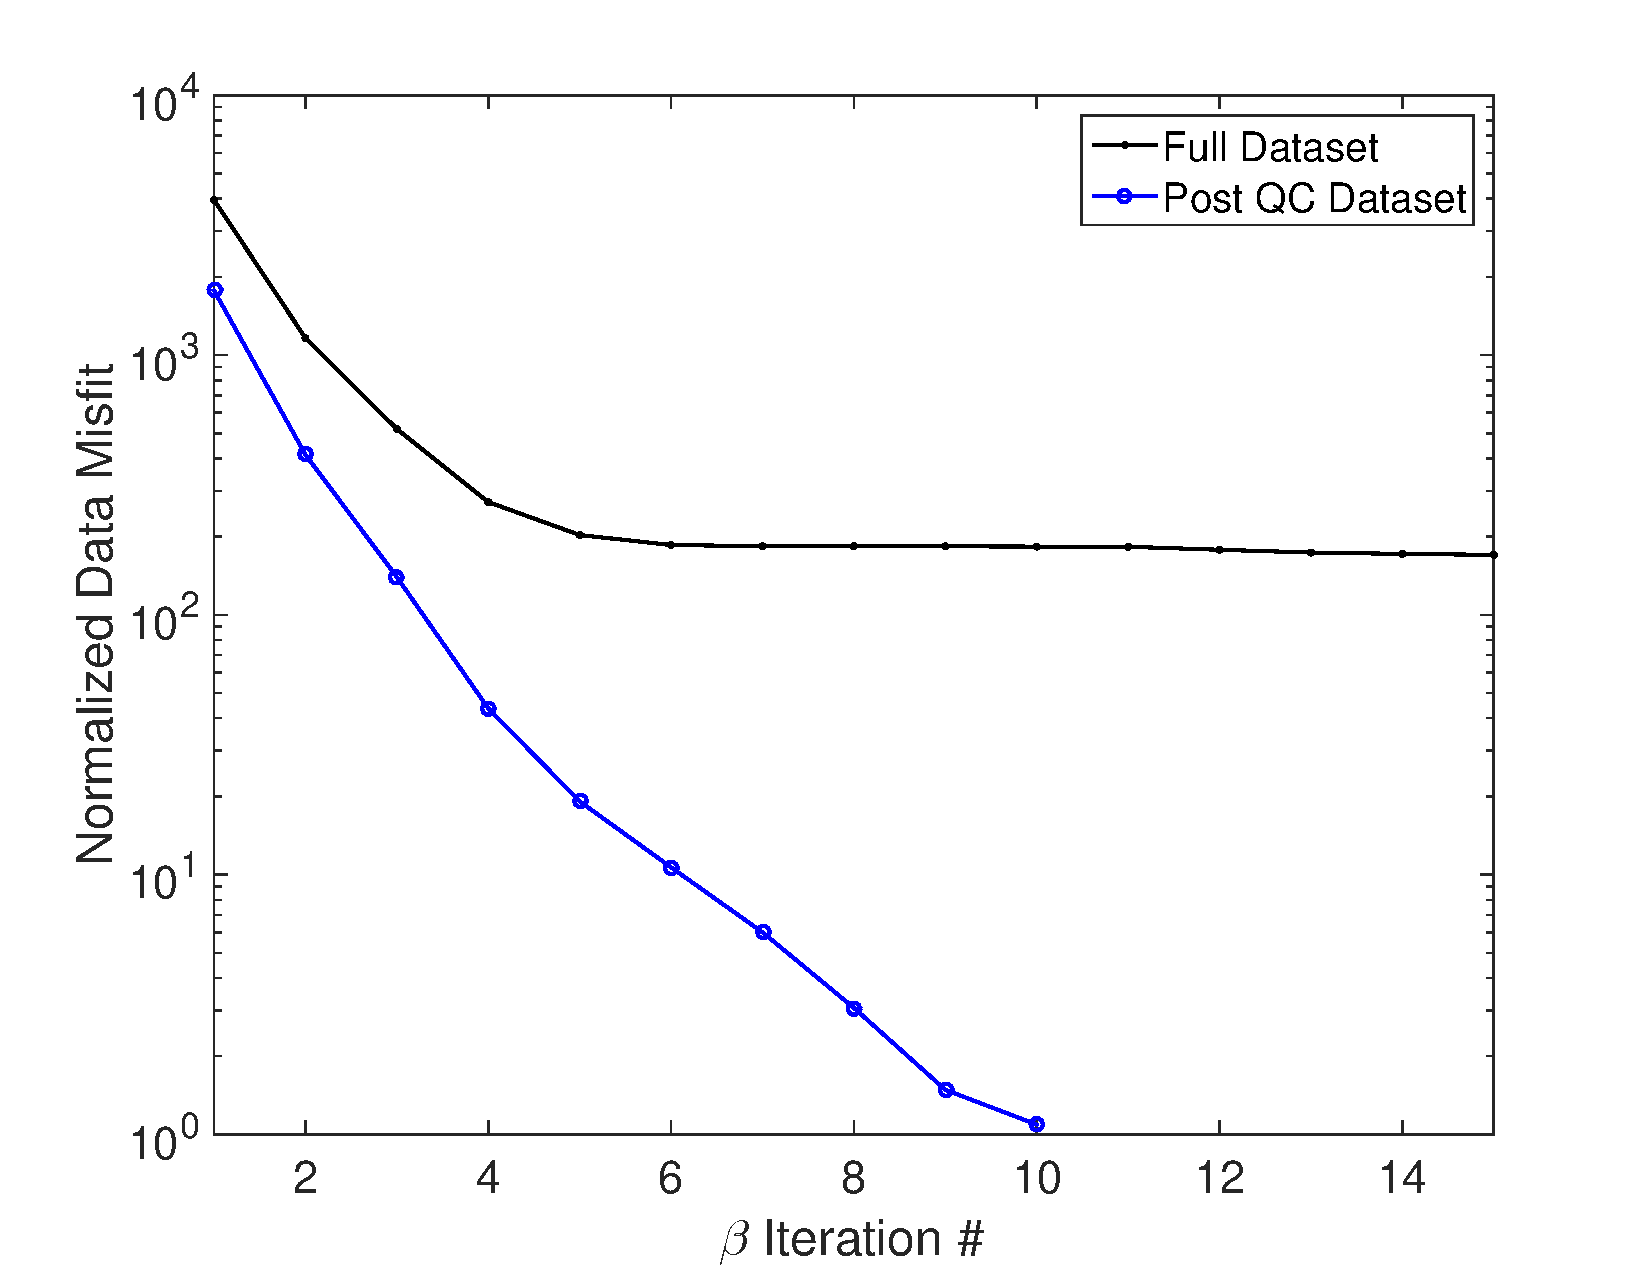
\includegraphics[trim=1.3cm 0.2cm 2.6cm 1.2cm, clip=true,width=0.75\linewidth]{./Figures/Fig18.pdf}
	\end{center}
\caption{Normalized data misfit curves from the initial inversion and the post-QC inversion. While the initial inversion struggles to fit the observed data the inversion of the post-QC data subset reached target misfit after 10 iterations.}
\label{fig:CaseStudy_Inv_MisfitPlots}
\end{figure}

Anomaly A closely follows the location of old mine workings, whose location is marked by the black lines in Figure \ref{fig:CaseStudy_InvMod_Final}, to the north west where it passes over the current mine working and connects with Anomaly D. This old section of tunnel was grouted off (sealed with concrete) at its southern end due to flooding. These inversion results indicate that this old section of tunnel still contains a substantial amount of brine. Anomalies E and F extend downward from the level of the mine workings. In both of these regions there were large quantities of standing water. The $\bigoplus$ symbols mark the location of conductive structures in the recovered model which extend upwards towards the Second Red Bed. In these localities we believe that water is seeping down into the salt from the overlying aquifer to form conductive anomalies A and B. It is possible that the water, in conductive zones A and B, then flows through old mine workings or dissolution conduits to the region around anomalies D-F where it accumulates and slowly seeps downwards.  

In the southern portion of the survey region there is another conductive region, anomaly C, which extends upwards. This is another region where water may be seeping into the mine from the aquifer above. Although there is also evidence of seepage into the mine workings at the far western end of this main tunnel, there is little evidence of this in the recovered conductivity model. Since this region is on the edge of our electrode array we may lack the resolution to resolve this target.

When interpreting these model results we need to be mindful of model resolution limitations which result from most of the electrodes being located along a single depth plane. Throughout the main tunnels there is 5m of variation in the elevation of electrodes. Off to the southeast 3 electrodes were also placed in a raise, approximately 20m higher than the main tunnel level. This variation in the elevation of electrodes helps provide some resolution in the z-direction. However, there is still a danger of the inversion mis-locating conductive anomalies due to the distribution of sensitivities. Conductive bodies above or below the mine level could potentially result in artifacts along the plane of higher sensitivities at the main tunnel level. Alternatively, model structures could also be pushed or smeared outwards into portions for the model which are poorly constrained by the data.   

To quantify the resolution of our model we used a probing technique, studied by \cite{Bekas2007}, to estimate the diagonal of the model resolution matrix ($diag(\mathbf{R}) \approx diag(\mathbf{J}^{T}\mathbf{J})$, where $\mathbf{R}$ and $\mathbf{J}$ are the model resolution and sensitivity matrices respectively. Figure \ref{fig:ModRes_CableSplitCombined_Final} shows the approximate model resolution for the same depth slice shown in Figure \ref{fig:CaseStudy_InvMod}. Model resolution is highest near electrodes 61-120 on Cable 2 since there are fewer data associated with Cable 1 in the post-QC dataset due to the larger current leakage problems. Only slight reductions in model resolution are observed out to a distance of $10$m above or below the main tunnel level. These results improve our confidence in the recovered model since all of the interpreted anomalies fall within this 10m zone above or below the main tunnel level.

\begin{figure} [!ht]
    \begin{center}
       \label{fig:ModRes_CableSplitCombined_Final_z2586}
       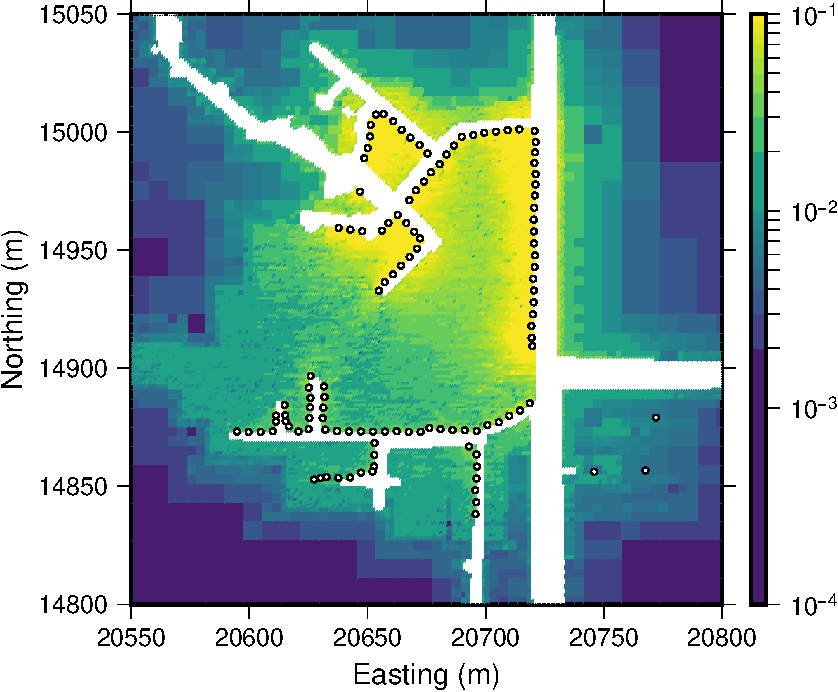
\includegraphics[trim=0cm 0cm 0cm 0cm, clip=true,width=0.95\linewidth]{./Figures/Fig19.pdf} 
    \end{center}
\caption{A plot showing the approximate model resolution for the depth section shown in Figure \ref{fig:CaseStudy_InvMod}. Higher resolution areas are focused around electrodes 61-120 which are connected with Cable 2. In the z-direction, only a small decrease in resolution is observed out to about 10m above or below the main tunnel level suggesting that structures within this region are constrained by the data.}
\label{fig:ModRes_CableSplitCombined_Final}
\end{figure}  
 
\section{Synthetic Testing}
\label{Synthetic_Testing}

To further test the applicability of our data QC methodology we tested it on a synthetic example in which three different types of contaminating noise were added. The synthetic model consists of a 10 m $\times$ 10 m $\times$ 20m long conductive block ($\sigma_{Block}= 10$ S/m) which is vertically centered in the central region between two legs of an asymmetric tunnel (See Figure \ref{fig:Synth_Horseshoe_RefMod}). The tunnels measure 3 m $\times$ 3 m in cross section. Both the tunnels and conductive block are hosted in a $1e^{-4}$ S/m full-space. As in the field example the electrodes are placed every 5 m along the interior walls of the tunnels. The electrodes are numbered 1 through 26 starting in the south-west and proceeding clockwise around the tunnel. A non-conventional dipole-dipole dataset, incorporating all possible dipole-dipole measurements without reciprocals, was forward modeled and 5\% Gaussian noise was added. The inversion results of this relatively uncontaminated dataset are shown in figure \ref{fig:Synth_Horseshoe_InvMod}. Under these normal noise conditions the inversion is able to fit the data and recover the location of the conductive block.  

\begin{figure} [!ht]
    \begin{center}
    \subfigure[True Model]{%
       \label{fig:Synth_Horseshoe_RefMod}
       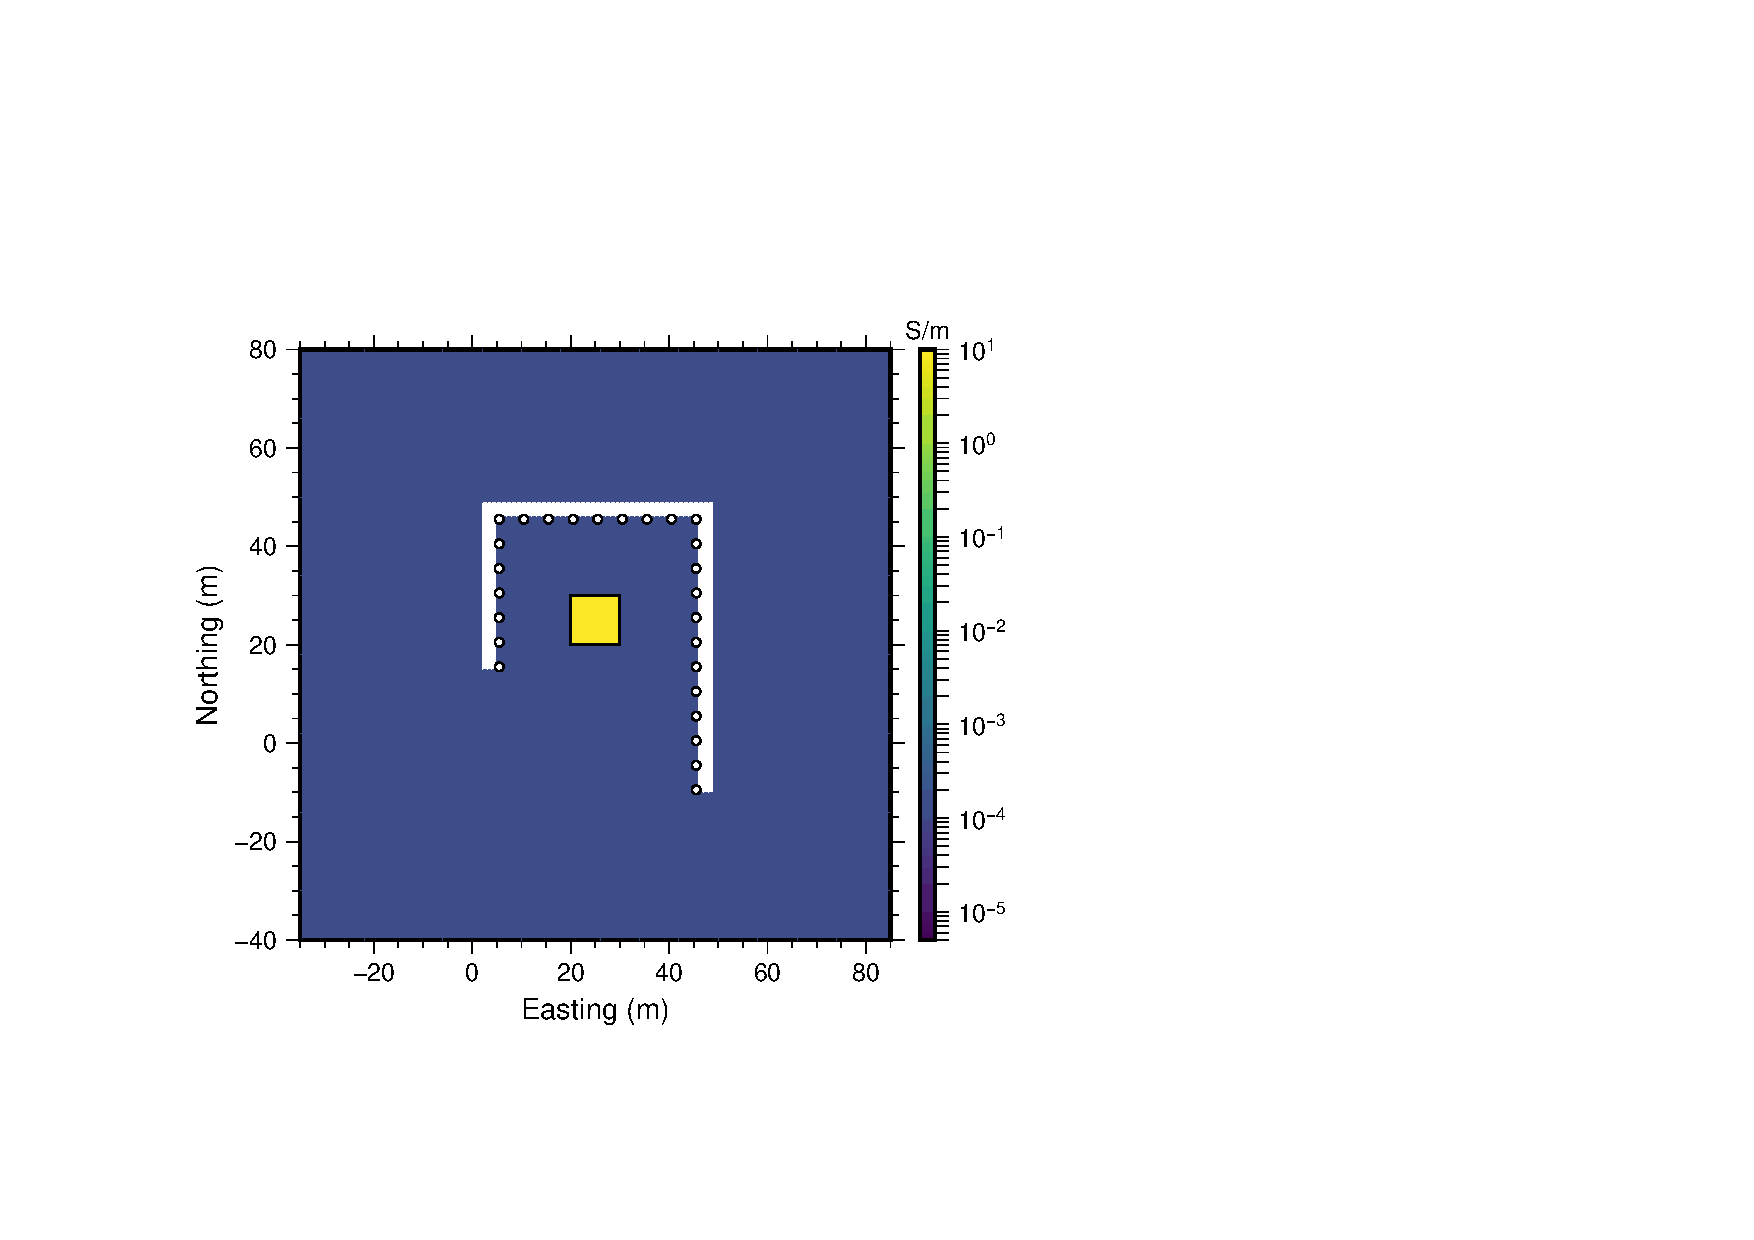
\includegraphics[trim=3.35cm 3.6cm 11.95cm 5.4cm, clip=true,width=0.475\linewidth]{./Figures/Fig20a.pdf}
       } %
    \subfigure[Recovered Model]{%
       \label{fig:Synth_Horseshoe_InvMod}
       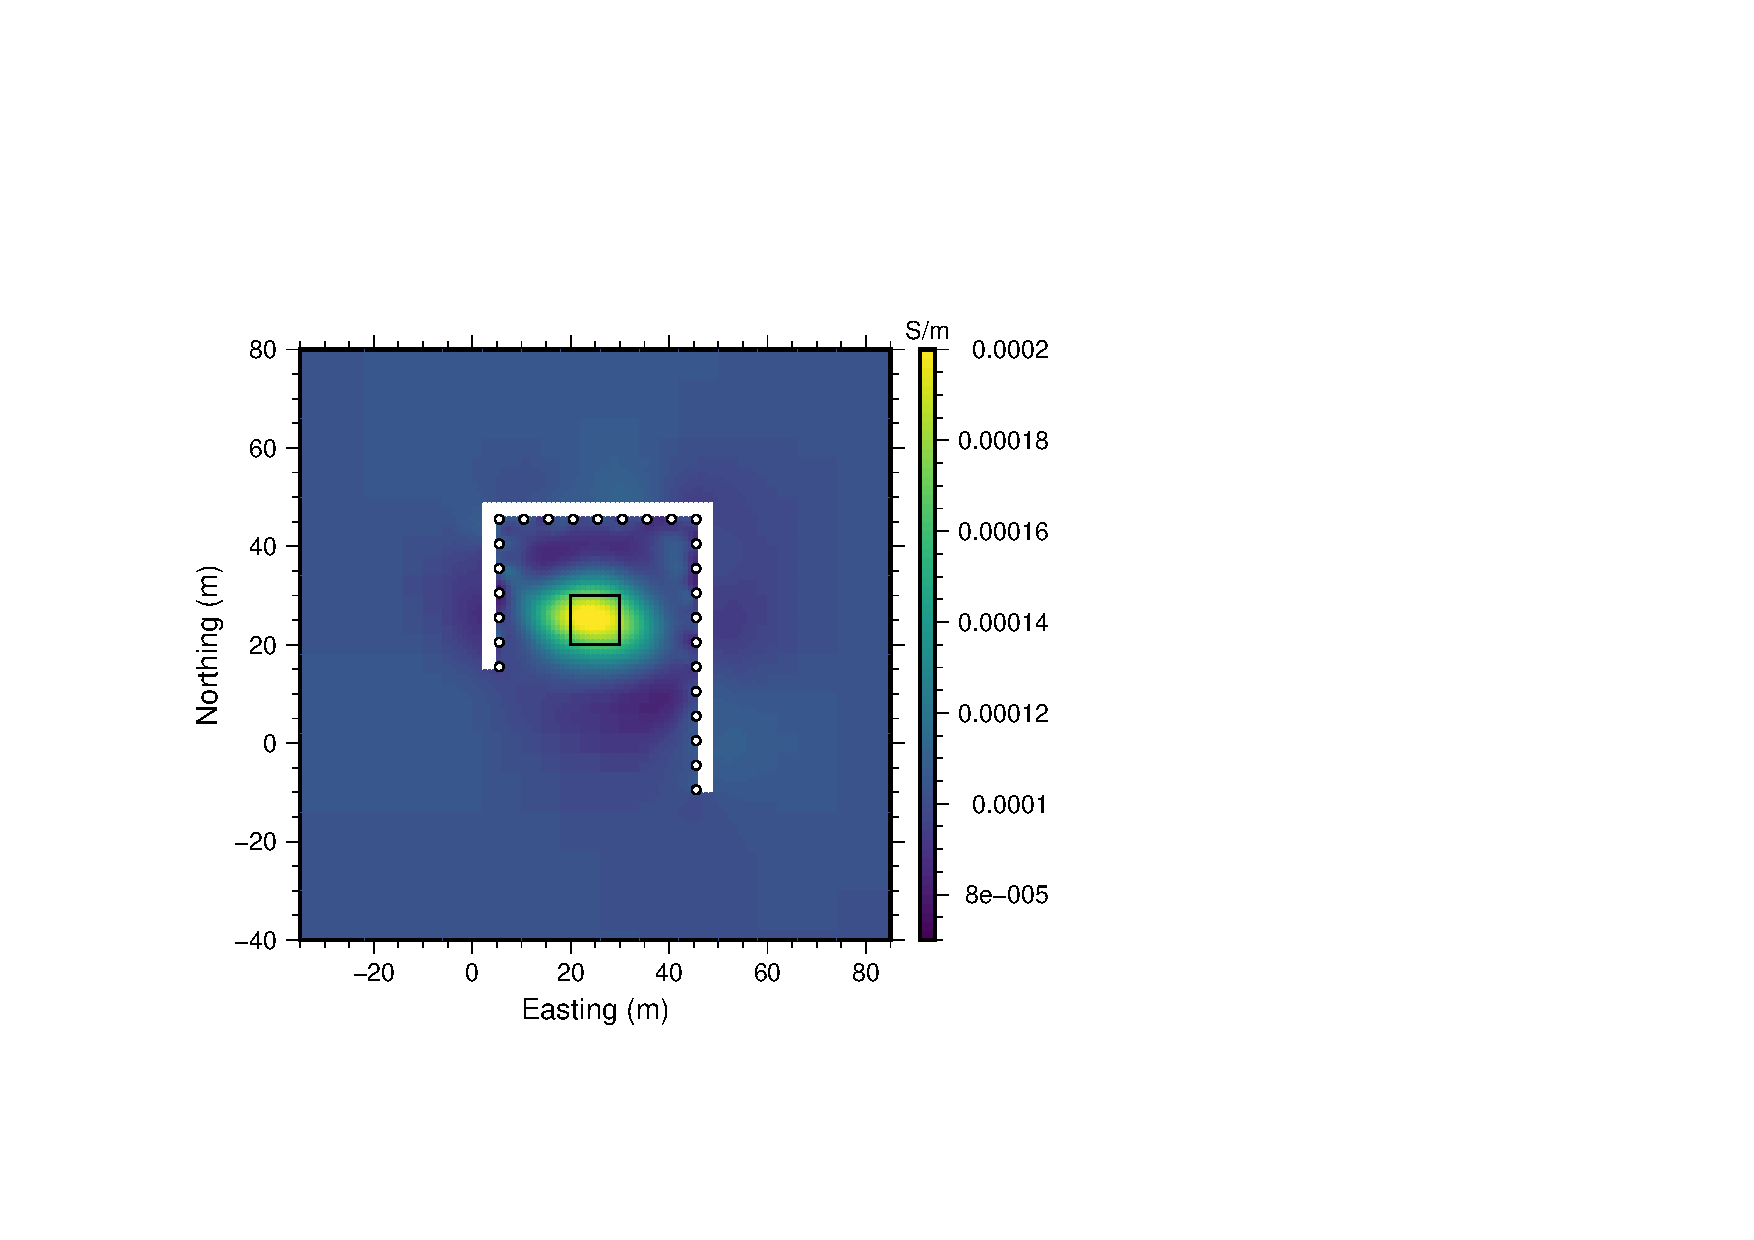
\includegraphics[trim=3.35cm 3.6cm 11.95cm 5.4cm, clip=true,width=0.475\linewidth]{./Figures/Fig20b.pdf}
       } %     
    \end{center}
\caption{A baseline synthetic study which shows how well the inversion is able to recover the conductive block under normal noise conditions, in which 5\% Gaussian noise was add to the forward modeled data. Both panels show depth slices through the model, which cut through the center of the tunnels and conductive block.}
\label{fig:Synth_HorseshoeModels}
\end{figure}

To evaluate the data QC methodology's ability to deal with some of the types of noise present in the field dataset, synthetic trials were set up to simulate the contaminating effects of a few troublesome electrodes, current leakages due to damaged cables or connection boxes, and the effects of infrastructure such as large steel pipes which are hung from the tunnel walls. Statistical measures of the noise present in the field dataset were used to contaminate the synthetic data. Estimations of the noise in the field data were made by computing the percent difference between normalized potentials ($d^{obs} = V_{MN}/I$) from the full field dataset and the forward modeled data from the final post-QC inversion result ($d^{pred}$). Subsets of the data were then analyzed to determine the distribution of percent differences in each subset. A best fitting Student-t location-scale probability distribution was fit to each distribution of percent differences. These probability distributions were then randomly sampled to create noise models for the synthetic data.

\subsection{Bad Electrodes Trial}

For the bad electrodes trial, characteristic noise models derived from the best fitting probability distribution for electrodes 15 and 113 in the field dataset were added to data associated with electrodes 5 and 24 in the synthetic dataset. The contaminated dataset was then put through the data QC process outlined above. In Stage I, it is possible to identify electrodes 5 and 24 as troublesome electrodes using both SVD analysis and boxplots similar to the one shown in Figure \ref{fig:Boxplot_Full_DataMisfit_vs_MElecID}. If all of the data associated with electrodes 5 and 24 are removed, the inversion is able to easily fit the remaining data. For comparison the full dataset was passed to Stage II where the clustering analysis was performed. After only 2 rounds of Stage III clustering the data QC process was completed. Figure \ref{fig:Synth_Horseshoe_BadElec} shows a comparison of the inversion models derived using the full bad electrode dataset, the dataset without any measurements from electrodes 5 or 24, the dataset after one round of cluster analysis, and the final post-QC dataset. 

\begin{figure} [!ht]
    \begin{center}
    \subfigure[Full Dataset]{%
       \label{fig:Synth_Horseshoe_BadElec_Full}
       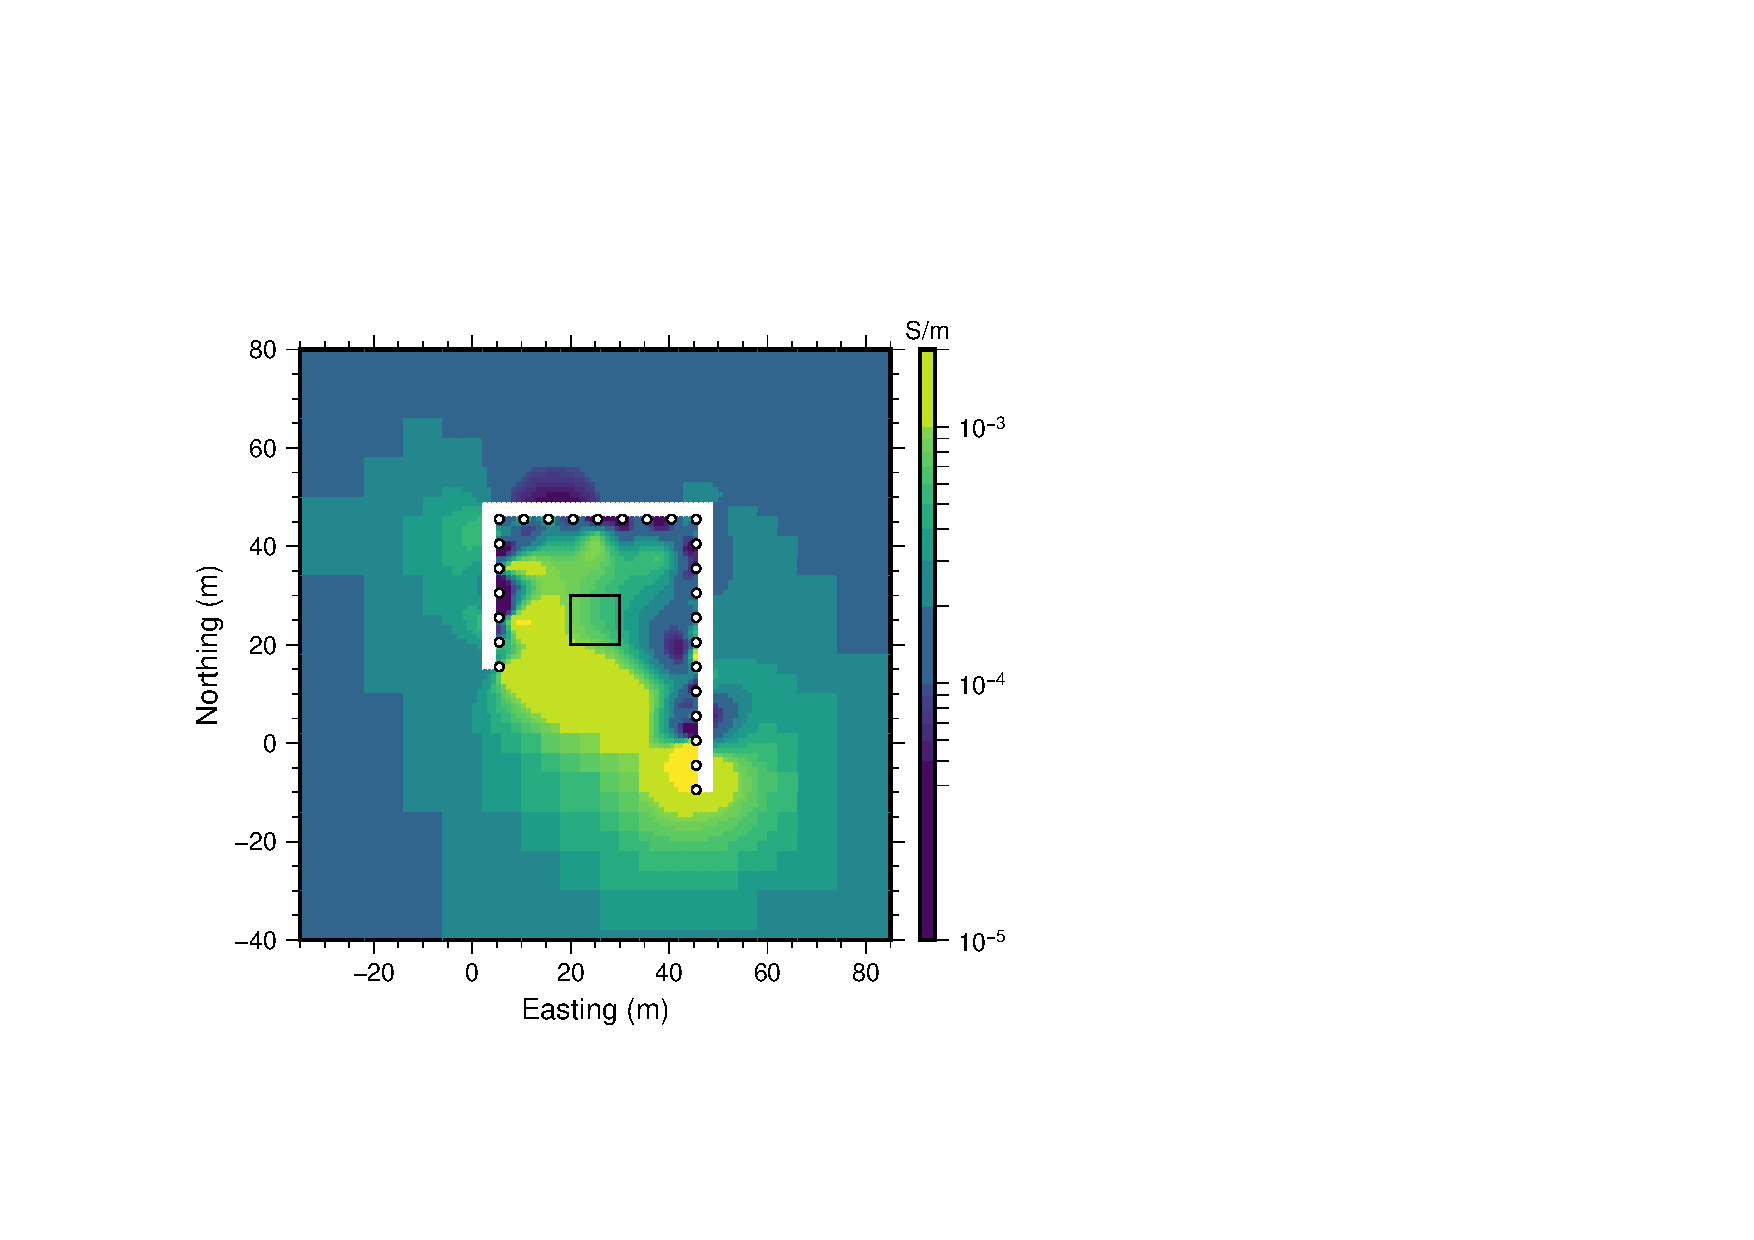
\includegraphics[trim=3.35cm 3.6cm 11.95cm 5.4cm, clip=true,width=0.475\linewidth]{./Figures/Fig21a.pdf}
       } %
    \subfigure[Removed Electrodes 5 and 24]{%
       \label{fig:Synth_Horseshoe_BadElec_No5_24}
       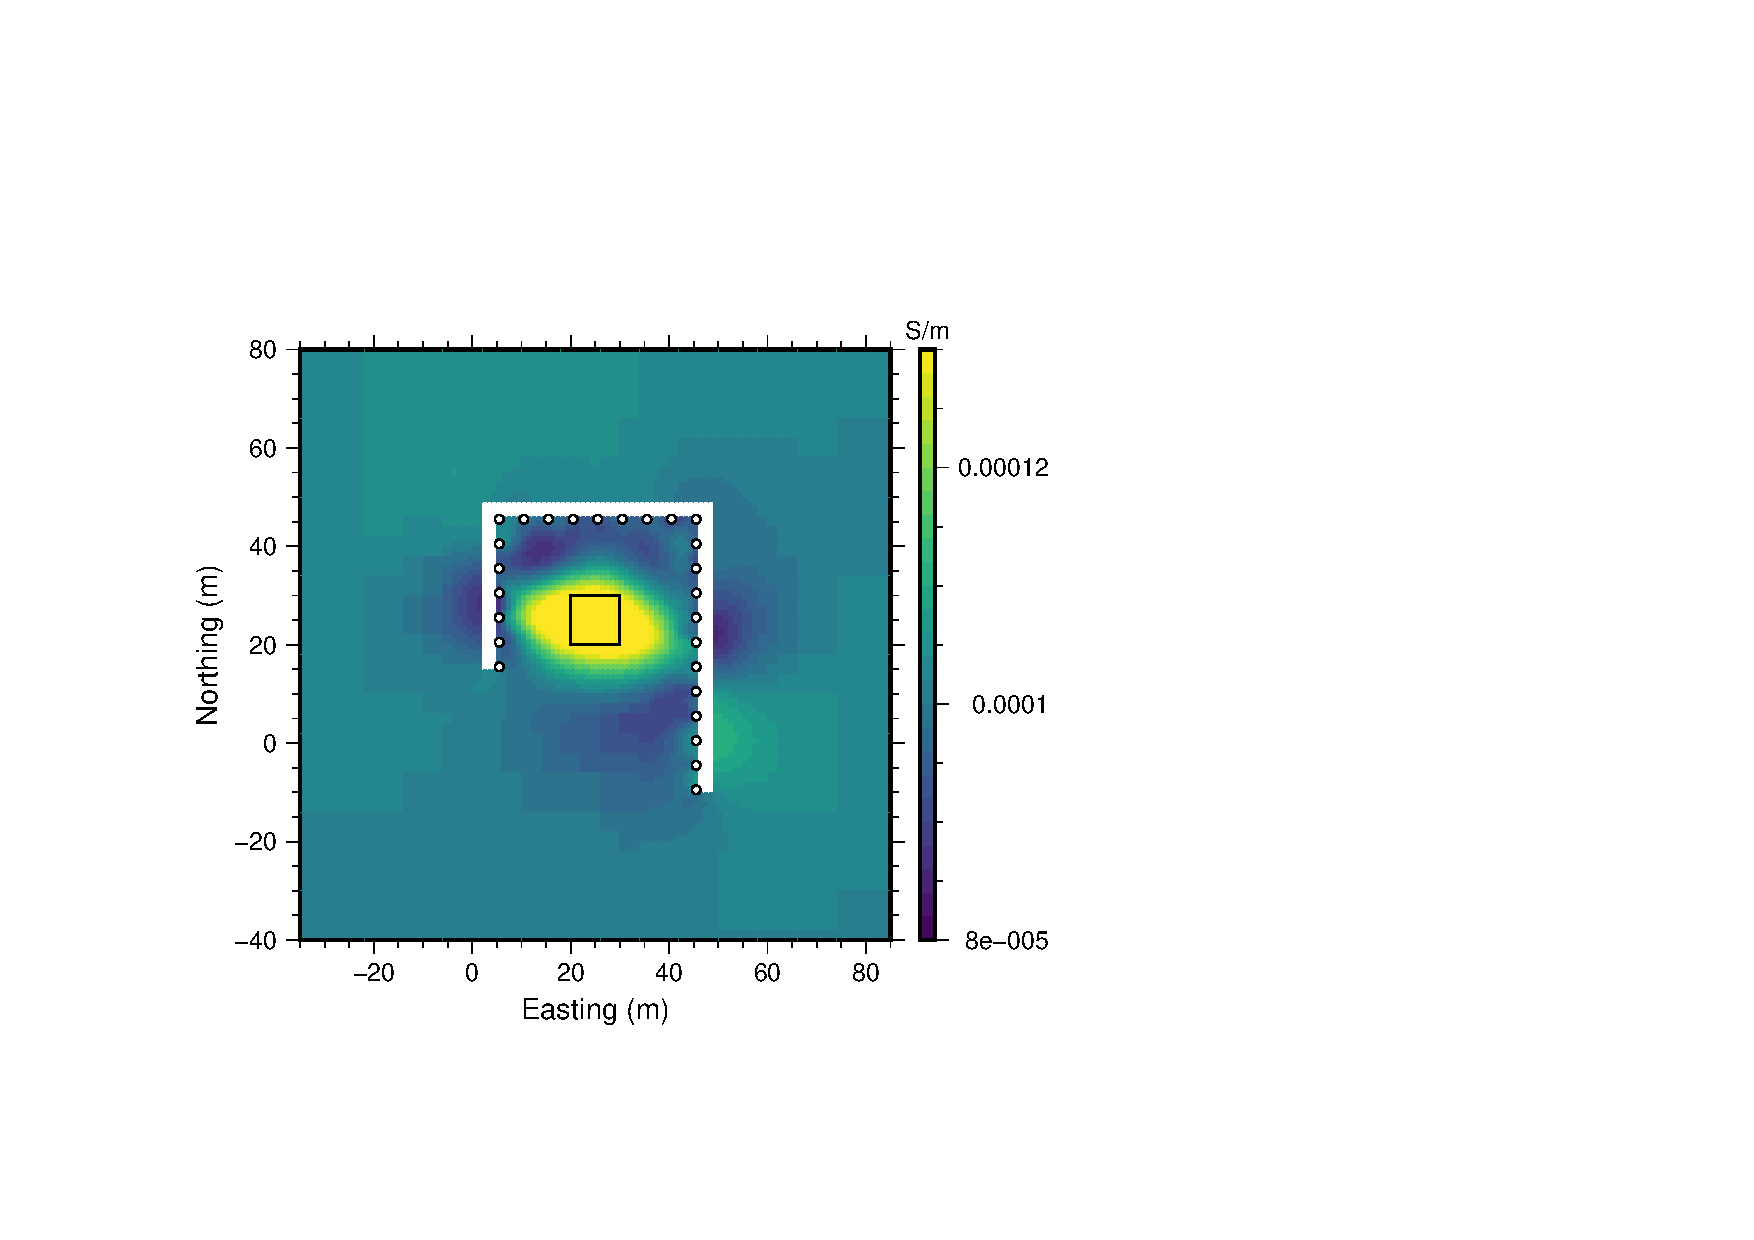
\includegraphics[trim=3.35cm 3.6cm 11.95cm 5.4cm, clip=true,width=0.475\linewidth]{./Figures/Fig21b.pdf}
       } \\%     
    \subfigure[Clustering (Stage III)]{%
       \label{fig:Synth_Horseshoe_BadElec_Clust}
       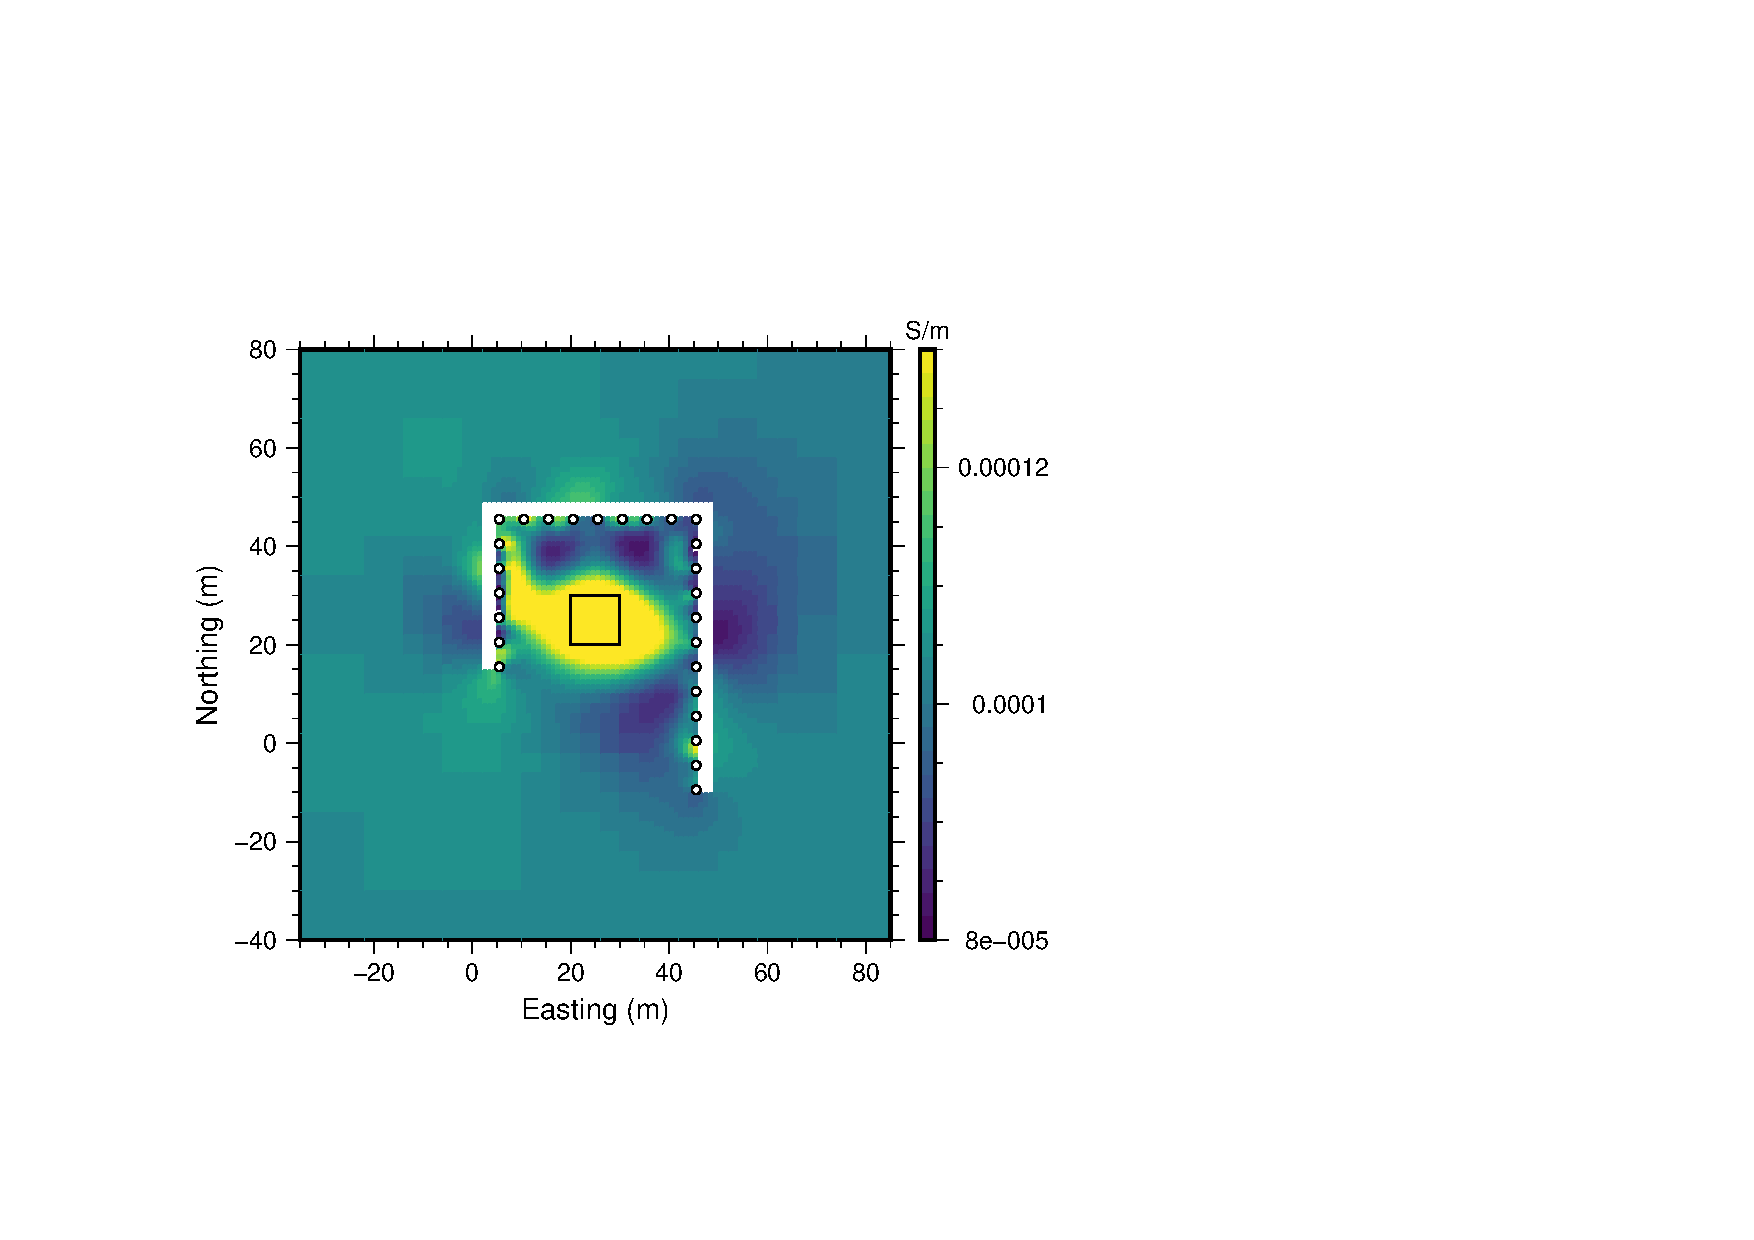
\includegraphics[trim=3.35cm 3.6cm 11.95cm 5.4cm, clip=true,width=0.475\linewidth]{./Figures/Fig21c.pdf}
       } %
    \subfigure[Clustering (Final)]{%
       \label{fig:Synth_Horseshoe_BadElec_ClustFinal}
       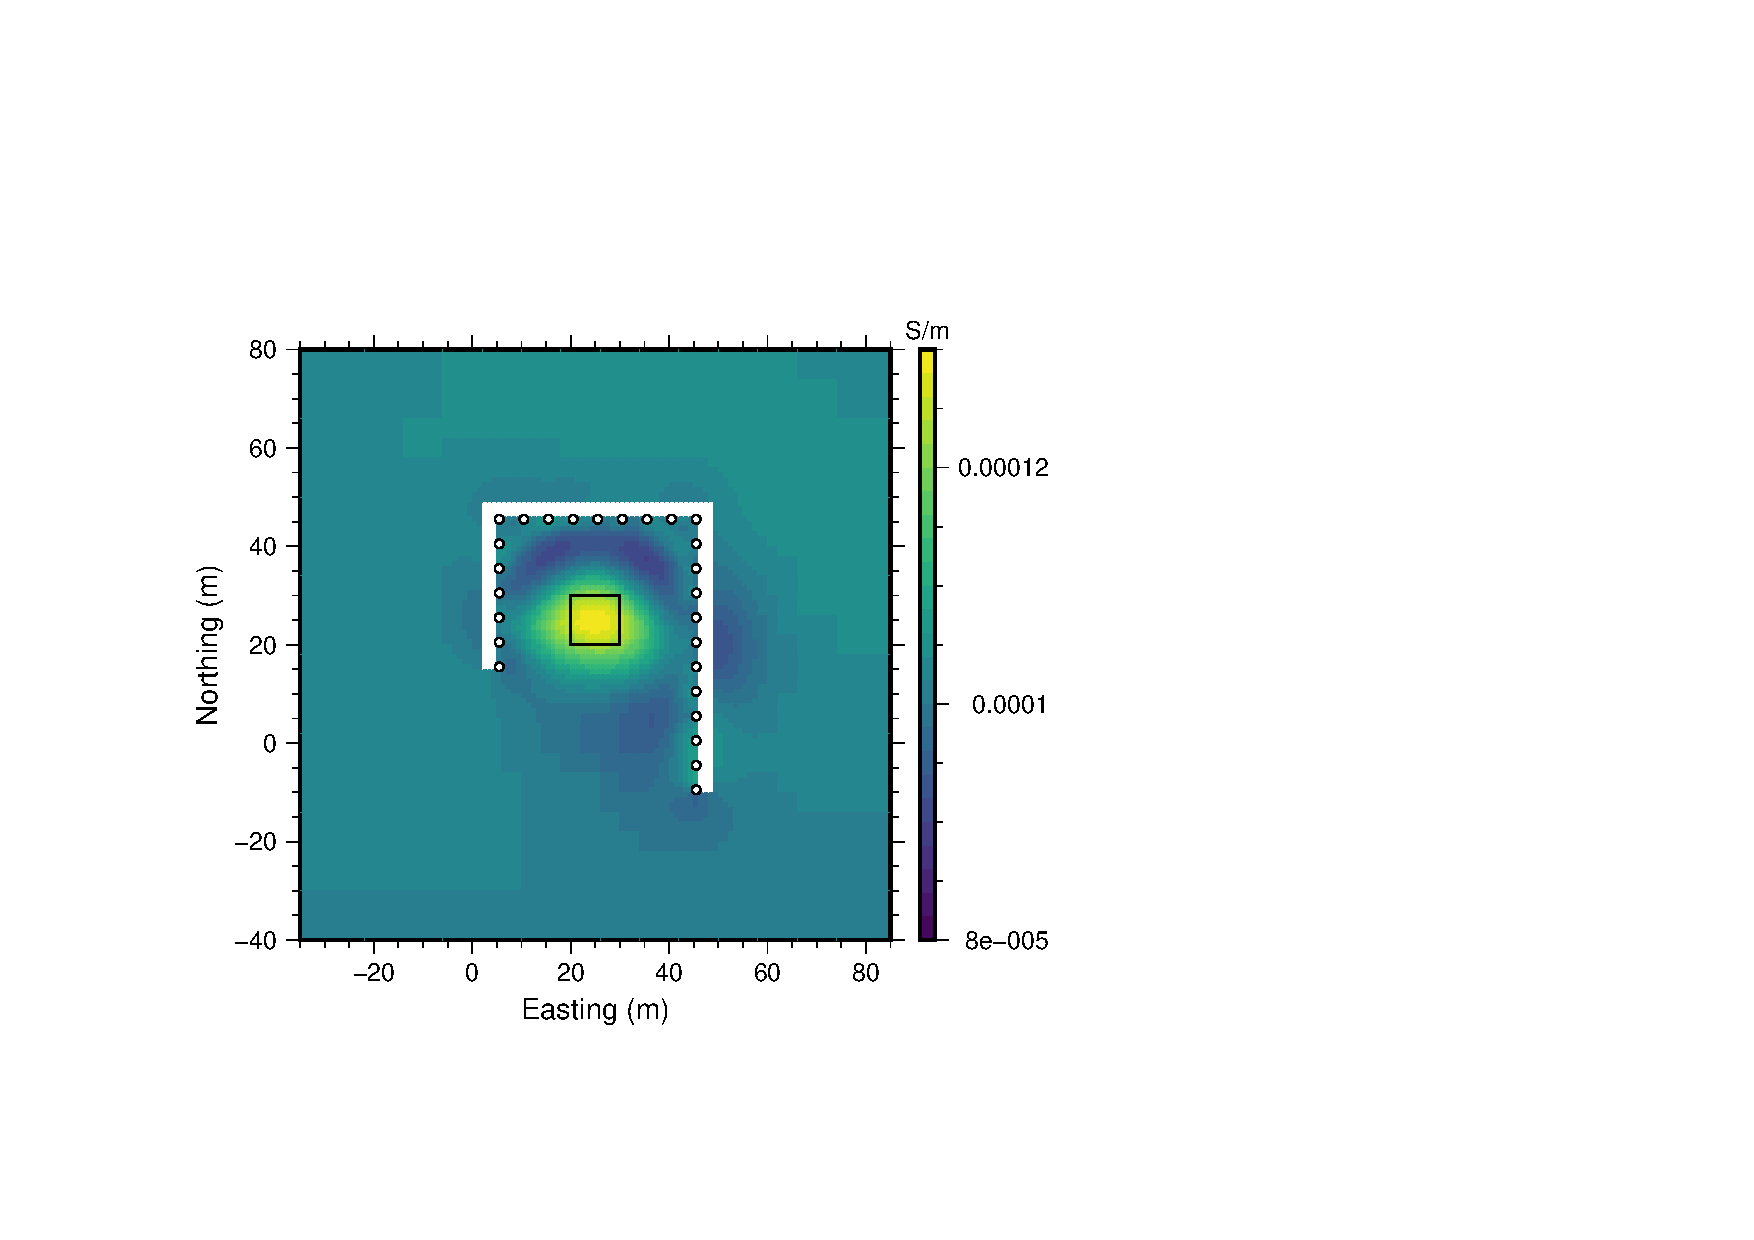
\includegraphics[trim=3.35cm 3.6cm 11.95cm 5.4cm, clip=true,width=0.475\linewidth]{./Figures/Fig21d.pdf}
       } %   
    \end{center}
\caption{Inversion results from the bad electrodes trial. The panels show the progression of the recovered model at different stages of the data QC process. Although good results are attained by removing all measurements associated with electrodes 5 and 24, clustering analysis produces a model which utilizes nearly 8,600 more data and better resolves the shape of the conductive block.}
\label{fig:Synth_Horseshoe_BadElec}
\end{figure}

The normalized misfit curves for each inversion are shown in Figure \ref{fig:Synth_Horseshoe_BadElec_MisfitPlots}, and Table \ref{tab:Synth_BadElec_Sizes} lists the number of data used in each inversion. Although removing all of the data from the two troublesome electrodes allows the inversion to reach the target misfit this may be unnecessary. The results of the cluster analysis indicate that only about one third of the measurements associated with these electrodes were so contaminated with noise that they warranted discarding. By retaining an additional 8,584 measurements the final dataset from the clustering data QC process does a better job of resolving the shape of the conductive block. 

If all of the data associated with a specific electrode are believed to be highly contaminated by a particular noise source it is best to discard all of the data. However, the measurements may only be highly contaminated when a specific electrode is used as a TX electrode, a RX electrode, or when used in a specific configuration with other electrodes. In these types of situations, cluster analysis is an effective tool for discriminating between highly contaminated and usable data.     

\begin{table}[!ht]
\small
\begin{center}
  \begin{tabular}{| c | c | c |}
    \hline
    \bf{Bad Electrodes Dataset} & \bf{\# Data} &  \bf{\% Discarded} \\
    \hline
    Full & 44,850 & $0 \%$\\
    \hline
    No electrode 5 or 24 & 31,878 & $28.9 \%$\\ % 12,972 removed
    \hline
    Clustering (Stage III)) & 41,206 & $8.1 \%$\\
    \hline
    Clustering (Final) & 40,462 & $9.8 \%$\\ % 4,388
    \hline   
  \end{tabular}
\caption{Dataset sizes for the bad electrodes trial.}
\label{tab:Synth_BadElec_Sizes}
\end{center}
\end{table}    

\begin{figure} [!ht]
	\begin{center}
	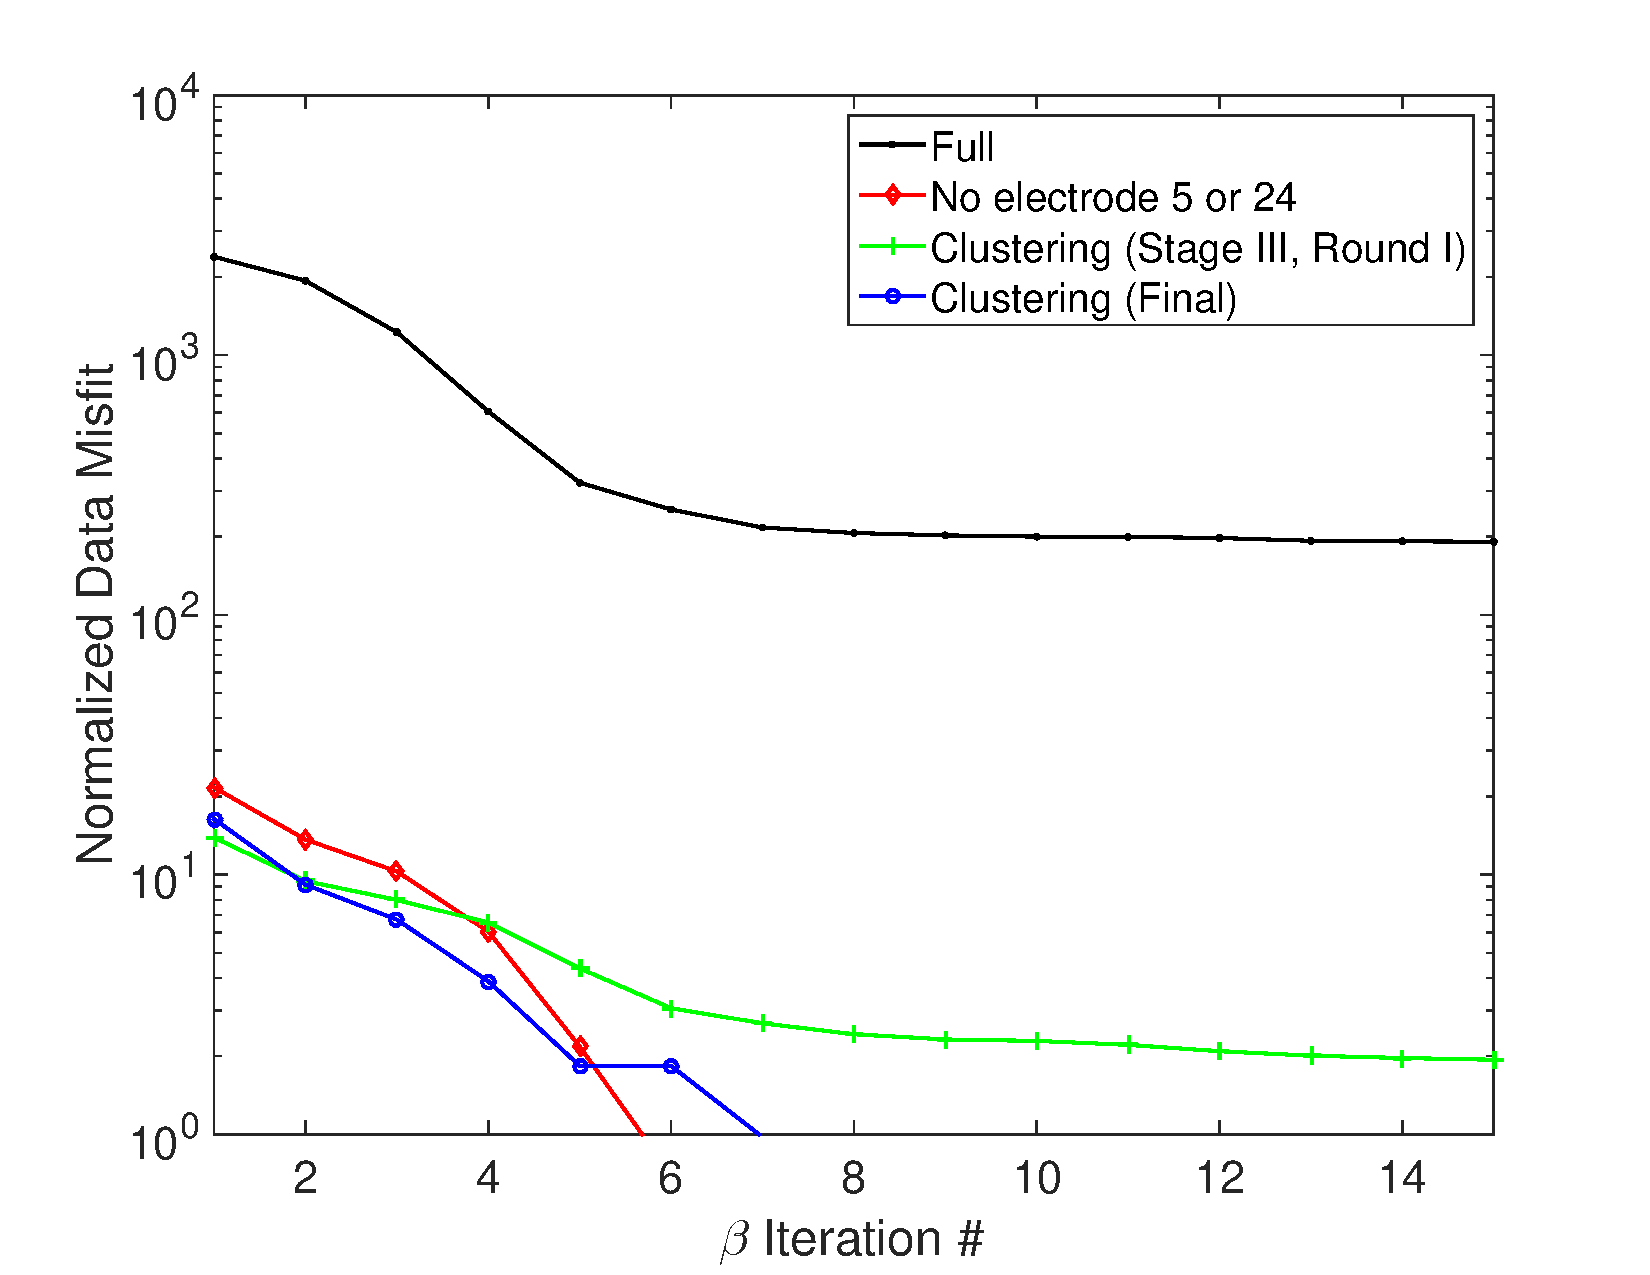
\includegraphics[trim=1.3cm 0.2cm 2.6cm 1.2cm, clip=true,width=0.75\linewidth]{./Figures/Fig22.pdf}
	\end{center}
\caption{This graph shows normalized data misfit curves for inversion results of the synthetic bad electrodes trial. While the inversion struggles to fit the full dataset the data QC methodology dramatically reduces the misfit so that misfits reach target levels for the subset in which all data associated with electrodes 5 and 24 were removed and the final dataset derived using clustering analysis.}
\label{fig:Synth_Horseshoe_BadElec_MisfitPlots}
\end{figure}

\subsection{Bad Cable Trial}

For the bad cable trial, noise based on the distributions observed in each of the cable split categories of the field data were added to the synthetic data in each corresponding category. The data QC methodology was then applied to the synthetic dataset in the same manner as the field dataset. Three rounds of Stage III clustering were required to obtain a final quality controlled dataset due to the very high levels of noise added to the data. The panels in Figure \ref{fig:Synth_Horseshoe_BadCable} show a progression through each of these rounds of clustering. 

In this trial there are radical changes in the recovered model from the initial inversion of the full dataset (panel \ref{fig:Synth_Horseshoe_BadCable_Full}) to the final post-QC inversion (panel \ref{fig:Synth_Horseshoe_BadCable_ClustFinal}). In the recovered model from the full dataset (panel \ref{fig:Synth_Horseshoe_BadCable_Full}) conductive material is concentrated along the western and northern sections of the tunnel. After the first round of Stage IV clustering, the conductive anomaly has shifted towards the central region between the tunnels but lies to the south of the true location of the conductive block. Small spacial scale positive and negative amplitude artifacts abound around electrode locations on the interior walls of the tunnel. In the final round of Stage IV clustering, the main conductive anomaly shifts northward towards the true location of the conductive block and artifacts are minimized.
\begin{figure} [!ht]
    \begin{center}
    \subfigure[Full Dataset]{%
       \label{fig:Synth_Horseshoe_BadCable_Full}
       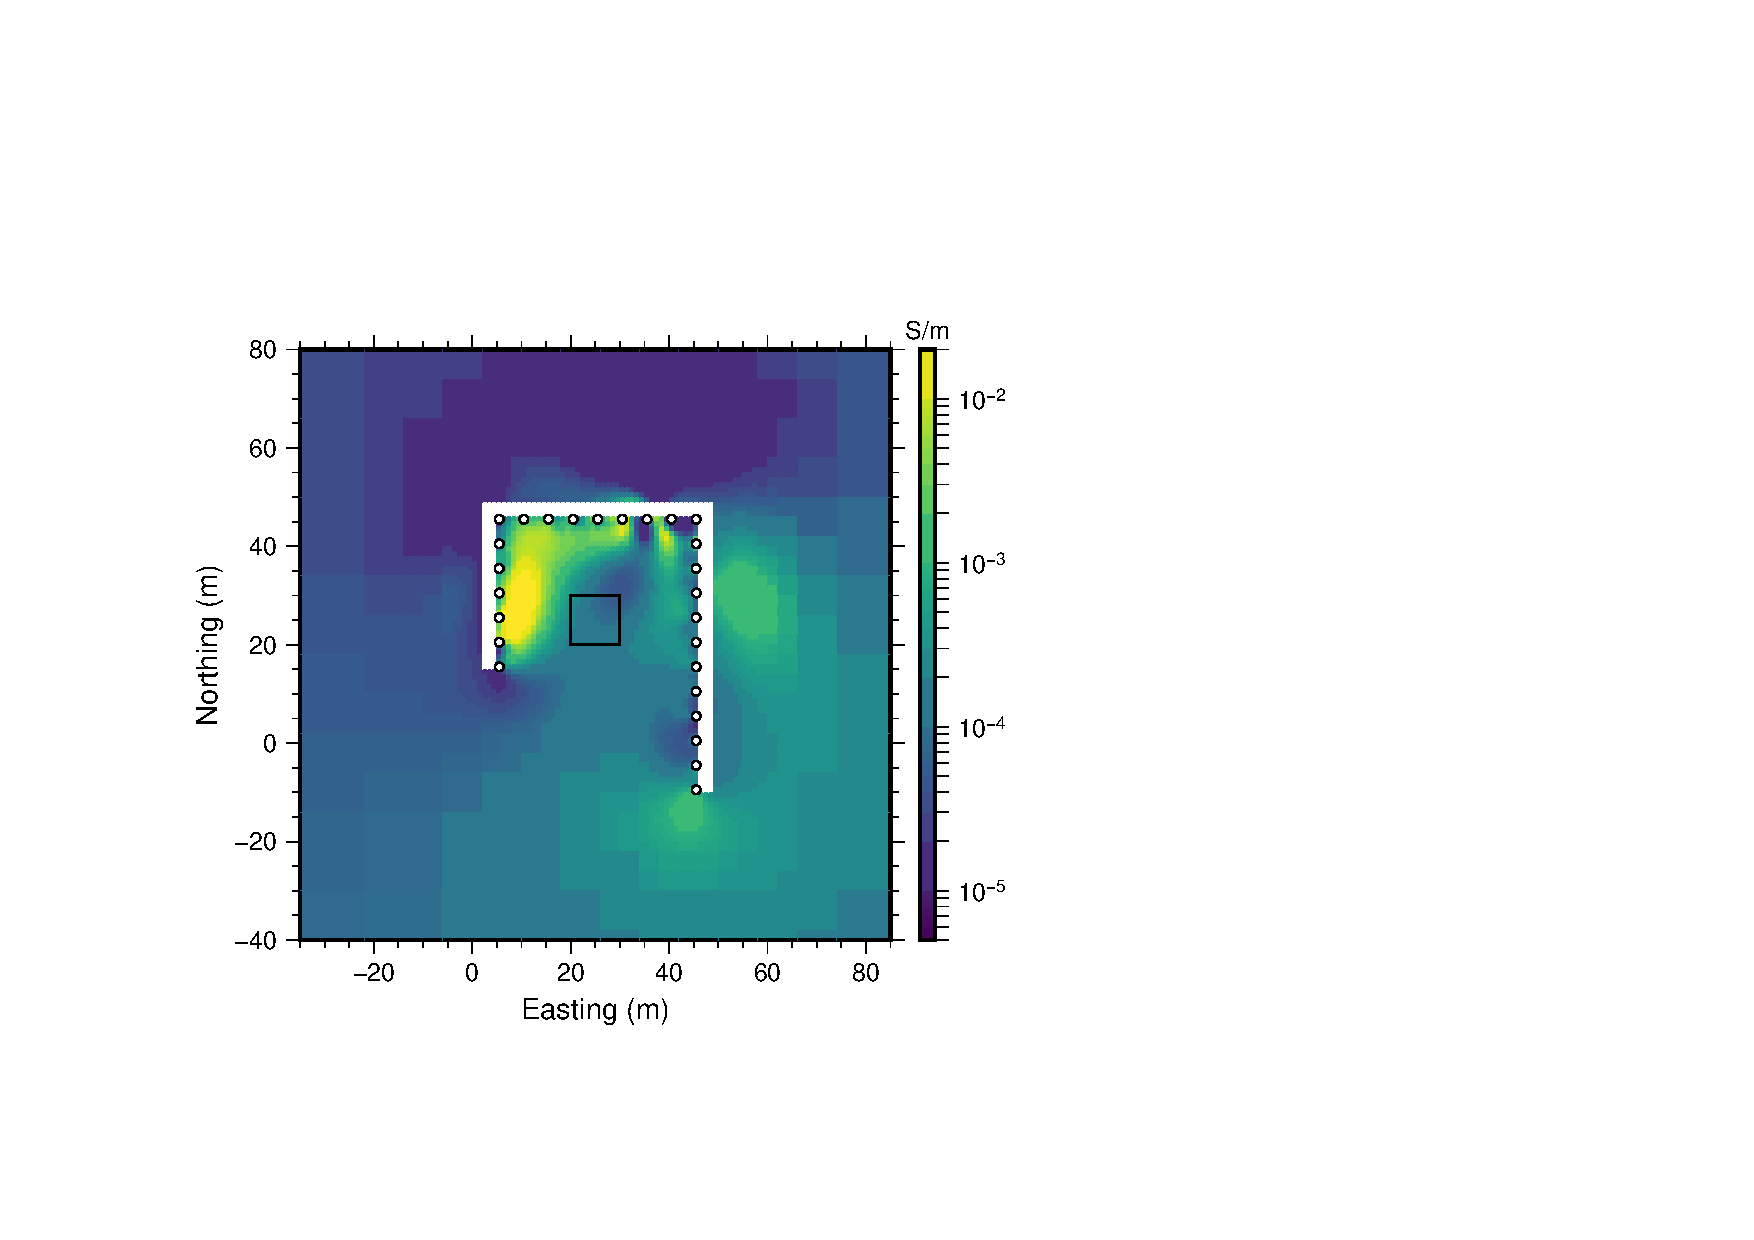
\includegraphics[trim=3.35cm 3.6cm 11.95cm 5.4cm, clip=true,width=0.475\linewidth]{./Figures/Fig23a.pdf}
       } %
    \subfigure[Clustering (Stage IV, Round I)]{%
       \label{fig:Synth_Horseshoe_BadCable_ClustStg2}
       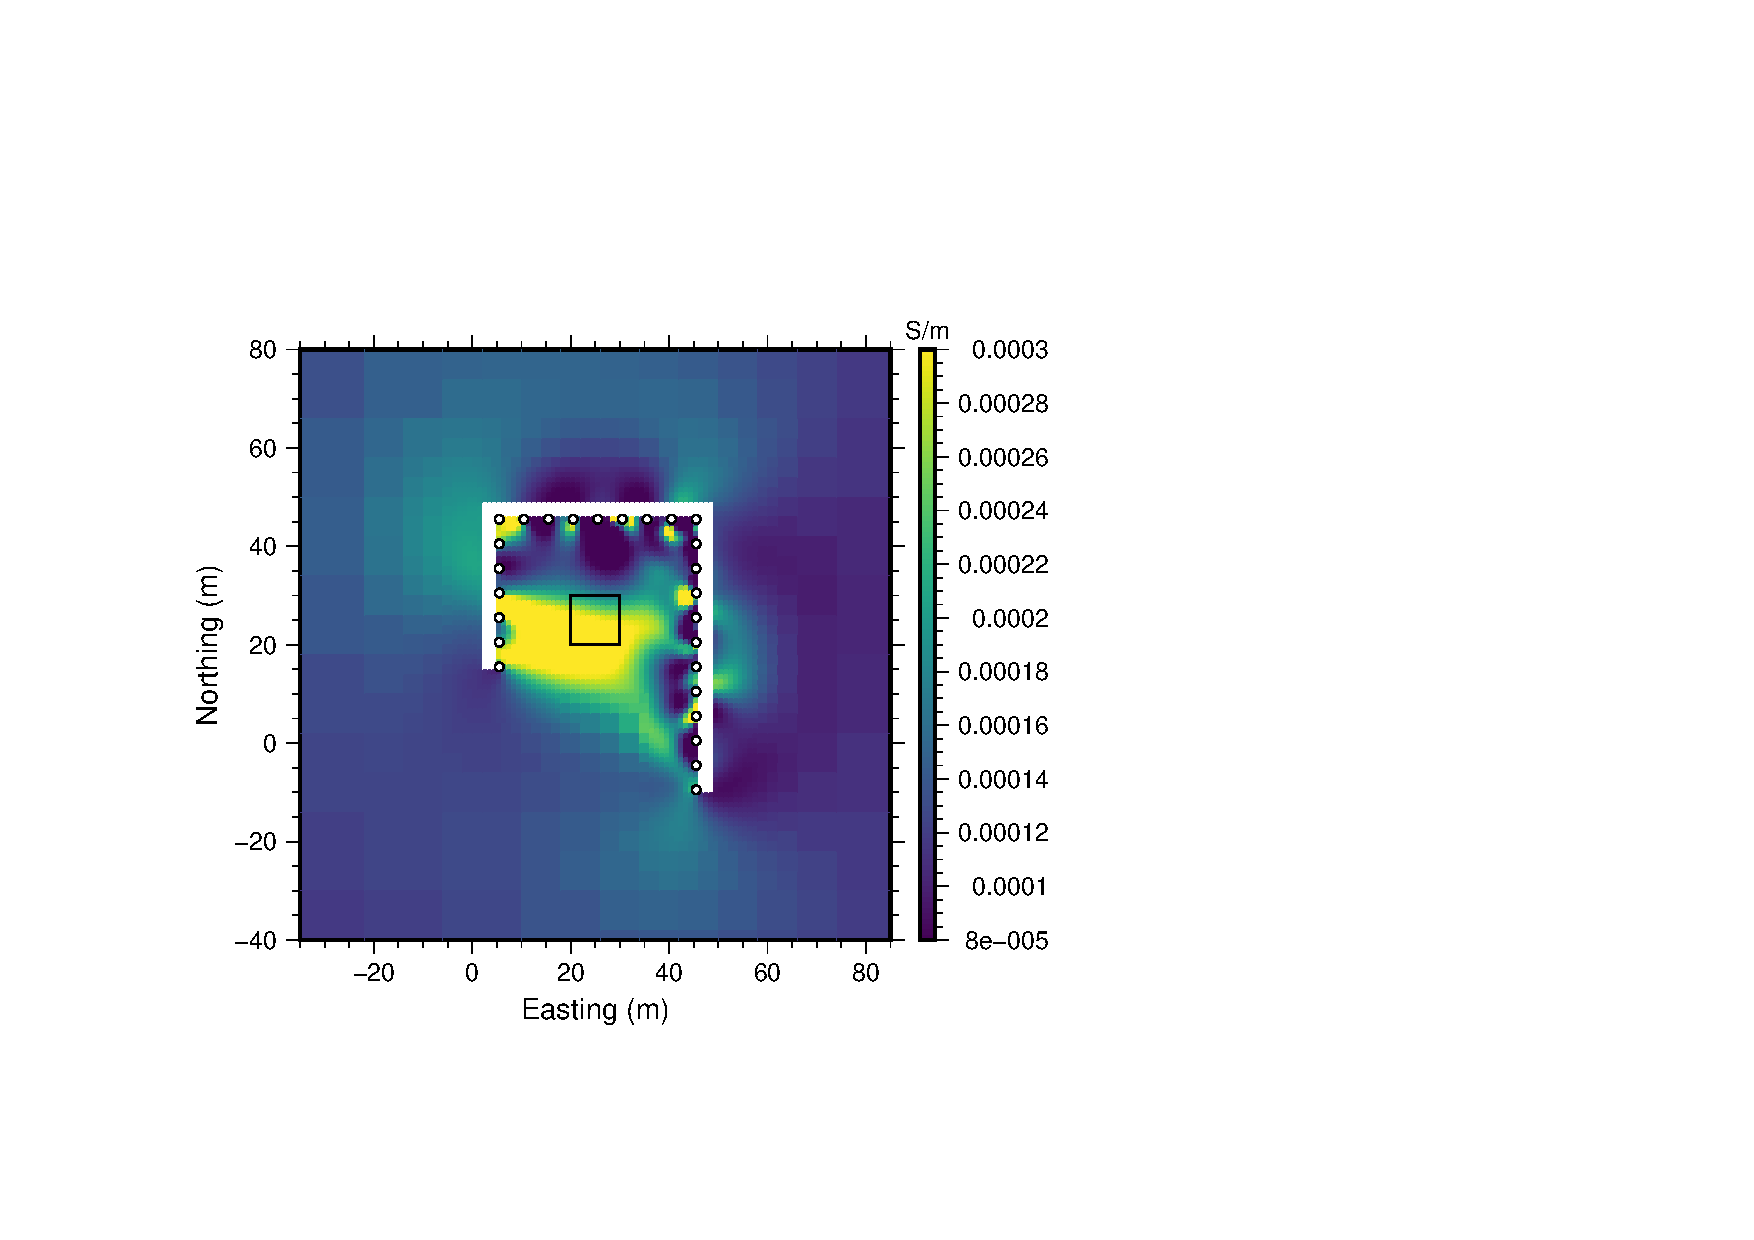
\includegraphics[trim=3.35cm 3.6cm 11.95cm 5.4cm, clip=true,width=0.475\linewidth]{./Figures/Fig23b.pdf}
       } \\%     
    \subfigure[Clustering (Stage IV, Round II)]{%
       \label{fig:Synth_Horseshoe_BadCable_ClustStg3}
       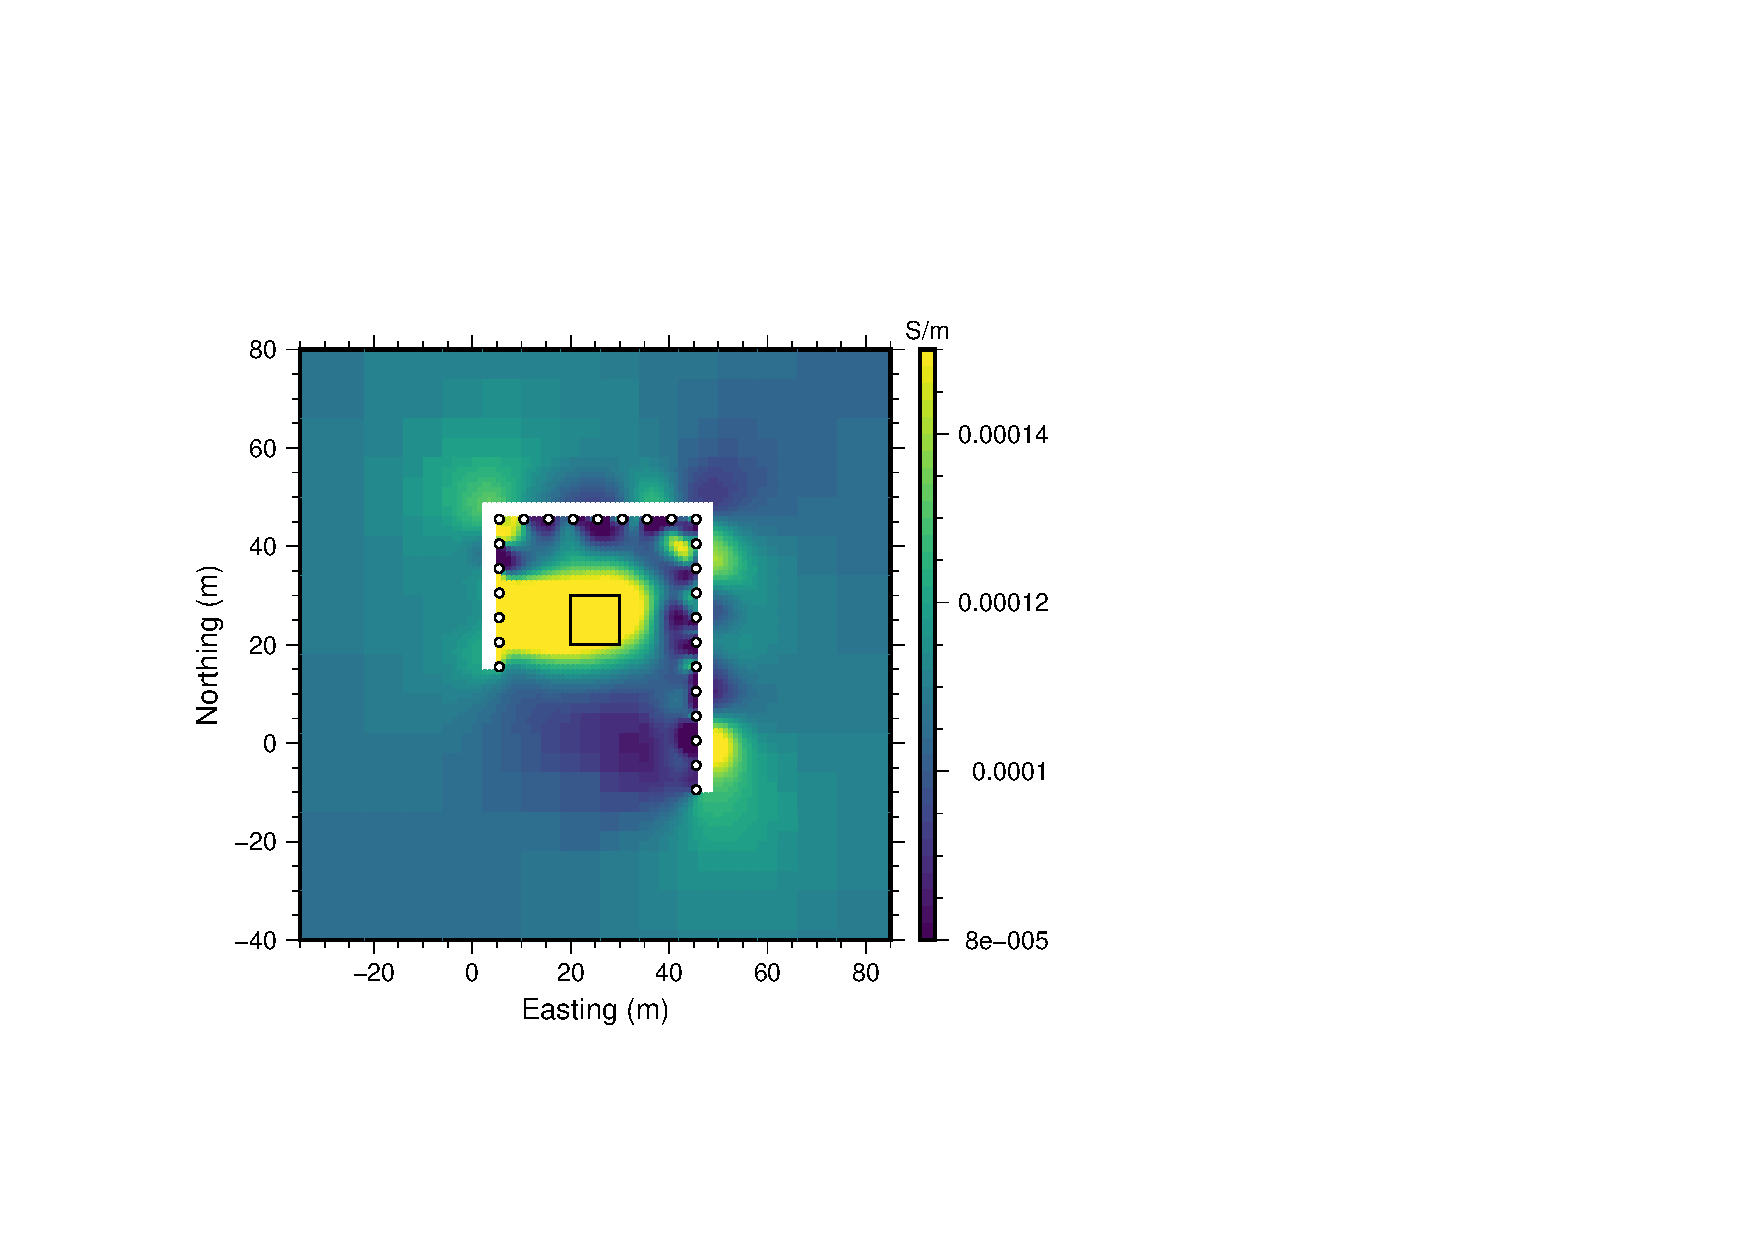
\includegraphics[trim=3.35cm 3.6cm 11.95cm 5.4cm, clip=true,width=0.475\linewidth]{./Figures/Fig23c.pdf}
       } %
    \subfigure[Clustering (Final)]{%
       \label{fig:Synth_Horseshoe_BadCable_ClustFinal}
       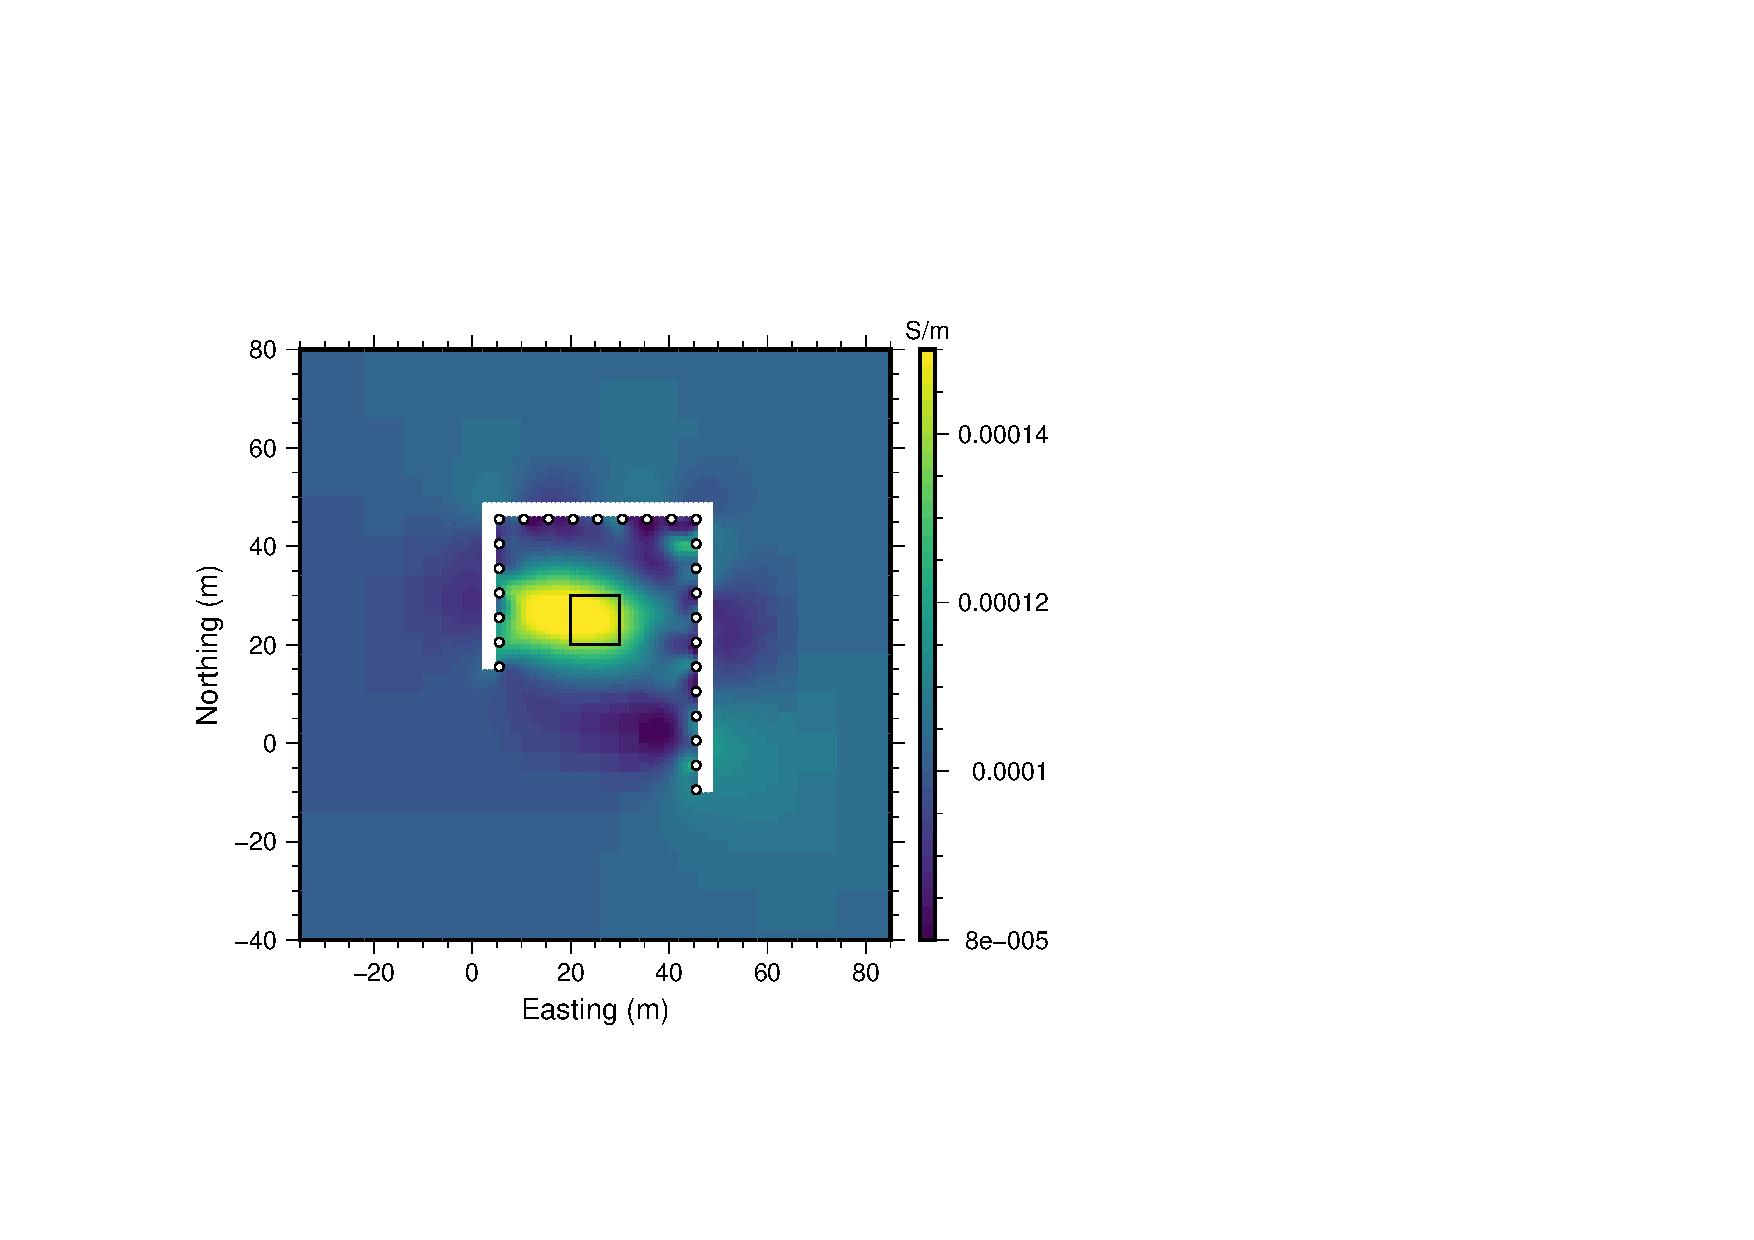
\includegraphics[trim=3.35cm 3.6cm 11.95cm 5.4cm, clip=true,width=0.475\linewidth]{./Figures/Fig23d.pdf}
       } %   
    \end{center}
\caption{These figures shows the incremental improvements in the recovered model after each round of clustering analysis for the highly noise-contaminated data in the bad cable trial. As the highly contaminated or inconsistent data are filtered out or the uncertainties are adjusted the location of the conductive anomaly shifts closer to the true location of the conductive block and many of the small scale artifacts disappear.}
\label{fig:Synth_Horseshoe_BadCable}
\end{figure}

The normalized data misfit curves in Figure \ref{fig:Synth_Horseshoe_BadCable_MisfitPlots} show that the initial inversion really struggled to fit the data because it was so severely contaminated. Although extensive testing was conducted to adjust the uncertainties of problematic clusters, nearly 85\% of the data were excluded from the final inversion (refer to Table \ref{tab:Synth_BadCable_Sizes}). Despite the severity of the contamination the post-QC recovered model does a reasonably good job of recovering the location of the conductive block. The smearing out of the conductive anomaly to the west is likely due to a lack of sufficient data to constrain this portion of the model since so much of the data had to be discarded. 

\begin{table}[!ht]
\small
\begin{center}
  \begin{tabular}{| c | c | c |}
    \hline
    \bf{Bad Cable Dataset} & \bf{\# Data} & \bf{\% Discarded}\\
    \hline
    Full & 44,850 & $0 \%$\\
    \hline
    Clustering (Stage IV, Round I) &  13,779 & $69.3 \%$\\
    \hline
    Clustering (Stage IV, Round II) & 12,285 & $72.6 \%$\\
    \hline
    Clustering (Final) & 7,082 & $84.2 \%$\\
    \hline   
  \end{tabular}
\caption{Dataset sizes for the bad cable trial.}
\label{tab:Synth_BadCable_Sizes}
\end{center}
\end{table} 

\begin{figure} [!ht]
	\begin{center}
	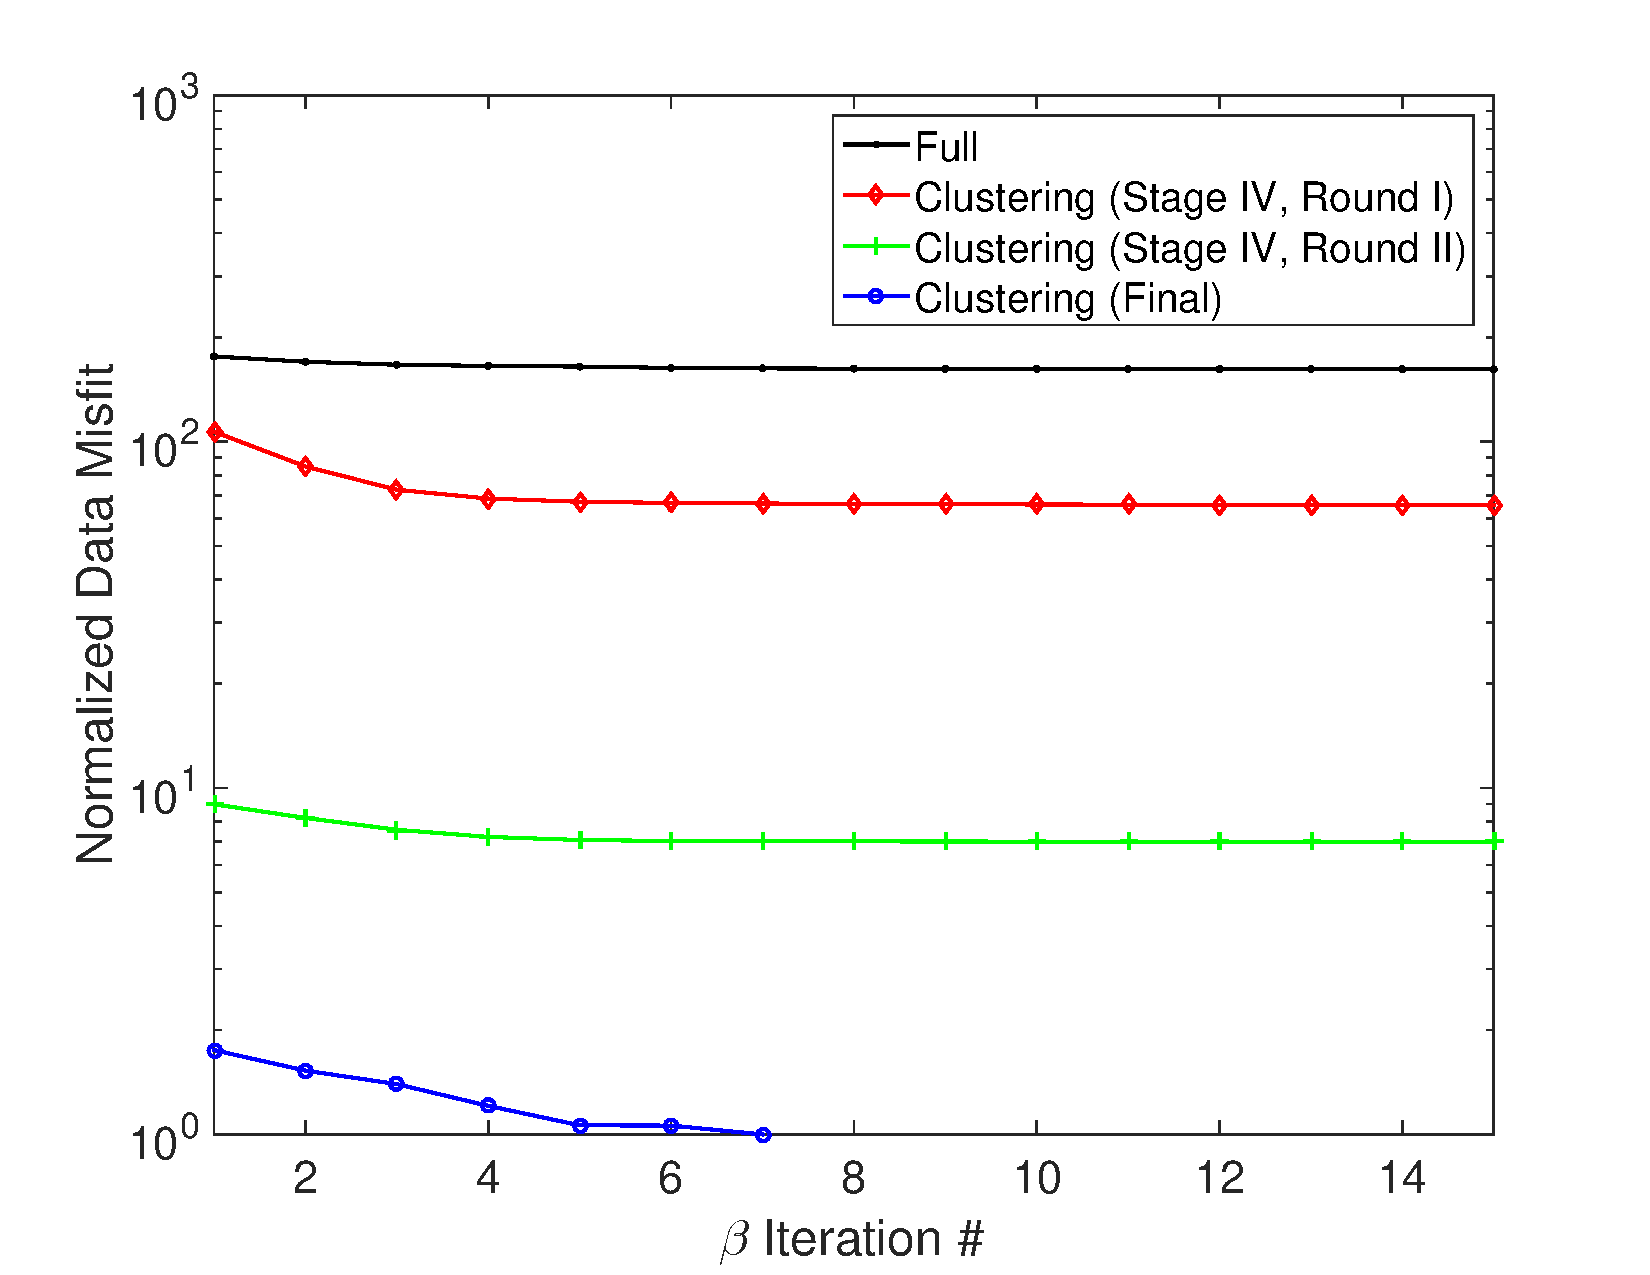
\includegraphics[trim=1.3cm 0.2cm 2.6cm 1.2cm, clip=true,width=0.75\linewidth]{./Figures/Fig24.pdf}
	\end{center}
\caption{Normalized data misfit curves, for the bad cable trial, that show the improvements in data fit with each round of clustering analysis. Due to the very high noise levels the misfit curves are fairly flat. The inversion of the final clustering subset is able to reach target misfit after 7 iterations.}
\label{fig:Synth_Horseshoe_BadCable_MisfitPlots}
\end{figure}

\subsection{Simulated Infrastructure Trial}

In the simulated infrastructure trial, a single cell thick conductive structure was added to the inside wall of the tunnel to simulate the presence of a large pipe or other infrastructure. This pipe-like structure runs along the eastern leg of the tunnel between electrode 16 and 20 (see Figure \ref{fig:Synth_Horseshoe_UniInfrastructure_RefMod}). A relative conductivity of about $2.2 \times 10^5$ S/m was assigned, which approximates the existence of a steel cylinder with a radius of 10 cm within the larger 1 m model cells. Synthetic data was forward modeled using the model with the ``pipe''. By inverting the data without taking the simulated infrastructure into account we can treat the signal from the thin conductive structure as a source of contaminating noise.

The results of the simulated infrastructure trial are shown in Figure \ref{fig:Synth_Horseshoe_UniInfrastructure}. As in the other trials, the inversion struggles to fit the full dataset and a number of artifacts are introduced into the recovered model in the vicinity of the pipe-like structure. In Stage I of the data QC process, boxplots similar to the one shown in Figure \ref{fig:Boxplot_Full_DataMisfit_vs_MElecID} and SVD analysis was used to search for sources of noise which are associated with specific electrodes. Measurements using electrodes 16-20 were found to be consistently associated with higher normalized misfits than other electrodes. Since these are the electrodes closest to the conductive ``pipe'' it seems logical that measurements utilizing these electrodes would be most impacted. If all of the data associated with electrodes 16-20 are removed, the inversion is able to easily fit the remaining data and the recovered model does a reasonably good job of resolving the conductive block as shown in panel \ref{fig:Synth_Horseshoe_UniInfrastructure_InvMod_NoElec16to20}. 

When the clustering analysis was carried out on the full dataset, a final quality controlled dataset was obtained after a single round of Stage III clustering. The recovered model (see panel \ref{fig:Synth_Horseshoe_UniInfrastructure_InvMod_Clustering}) shows that the clustering analysis only removed those data which were inconsistent and therefore difficult to fit. It did not completely remove the influence of the pipe-like conductor since a conductive anomaly is present between electrodes 16 and 20. If the location of infrastructure was documented during data acquisition, conductive anomalies such as this can be correctly attributed to infrastructure. Although a few small artifacts persist, the location and size of the conductive block are well resolved.  

\begin{figure} [!ht]
    \begin{center}
    \subfigure[True Model]{%
       \label{fig:Synth_Horseshoe_UniInfrastructure_RefMod}
       \includegraphics[trim=3.35cm 3.6cm 11.95cm 5.4cm, clip=true,width=0.475\linewidth]{./Figures/Fig25a.pdf}
       } %
    \subfigure[Full Dataset]{%
       \label{fig:Synth_Horseshoe_UniInfrastructure_InvMod_Full}
       \includegraphics[trim=3.35cm 3.6cm 11.95cm 5.4cm, clip=true,width=0.475\linewidth]{./Figures/Fig25b.pdf}
       } \\%
    \subfigure[Removed Electrodes 16-20]{%
       \label{fig:Synth_Horseshoe_UniInfrastructure_InvMod_NoElec16to20}
       \includegraphics[trim=3.35cm 3.6cm 11.95cm 5.4cm, clip=true,width=0.475\linewidth]{./Figures/Fig25c.pdf}
       } %     
    \subfigure[Clustering (Final)]{%
       \label{fig:Synth_Horseshoe_UniInfrastructure_InvMod_Clustering}
       \includegraphics[trim=3.35cm 3.6cm 11.95cm 5.4cm, clip=true,width=0.475\linewidth]{./Figures/Fig25d.pdf}
       } %
    \end{center}
\caption{A series of panels showing the results of the simulated infrastructure trial. While electrodes 16-20, which were closest to the pipe-like structure could be identified and removed as troublesome electrodes in Stage I of the data QC process clustering analysis leads to the removal of far fewer data. While nearly all evidence of the infrastructure have been removed from the inversion of the dataset without data from electrodes 16-20 the inversion of the final clustering dataset still prominently shows the location of the pipe. Trade-offs between improved model resolution due to better data coverage and possible interpretation complications related to infrastructure based anomalies need to be considered when processing the data.}
\label{fig:Synth_Horseshoe_UniInfrastructure}
\end{figure}

Normalized data misfit curves are shown in Figure \ref{fig:Synth_Horseshoe_UniInfrastructure_MisfitPlots} for each inversion, while the number of data in each dataset is summarized in Table \ref{tab:Synth_Infrastructure_Sizes}. While there is valuable signal contained in the additional 19,600 data retained in the final clustering dataset, the presence of infrastructure based anomalies can complicate the interpretation. This is especially true if the location of infrastructure is unknown or if conductive targets are in close proximity to the infrastructure. Care needs to be taken to differentiate the 2 types of anomalies; a comparison of \ref{fig:Synth_Horseshoe_UniInfrastructure_InvMod_NoElec16to20} and \ref{fig:Synth_Horseshoe_UniInfrastructure_InvMod_Clustering} may prove to be a useful tool for this.  

\begin{table}[!ht]
\small
\begin{center}
  \begin{tabular}{| c | c | c |}
    \hline
    \bf{Simulated Infrastructure Dataset} & \bf{\# Data} & \bf{\% Discarded} \\
    \hline
    Full &  44,850 & $0 \%$ \\
    \hline
    No electrodes 16-20 & 17,955 & $60.0 \%$ \\
    \hline
    Clustering (Stage III) & 38,144 & $15.0 \%$ \\
    \hline
    Clustering (Final) & 37,552 & $16.3 \%$ \\
    \hline   
  \end{tabular}
\caption{Dataset sizes for the simulated infrastructure trial.}
\label{tab:Synth_Infrastructure_Sizes}
\end{center}
\end{table} 

\begin{figure} [!ht]
	\begin{center}
	\includegraphics[trim=1.3cm 0.2cm 2.6cm 1.2cm, clip=true,width=0.75\linewidth]{./Figures/Fig26.pdf}
	\end{center}
\caption{Normalized data misfit curves for the simulated infrastructure trial which show that both the final clustering inversion and the inversion of the dataset with measurements from electrodes 16-20 removed are able to reach target misfit where the inversion of the full dataset struggles to fit the signal associated with the pipe-like conductor.}
\label{fig:Synth_Horseshoe_UniInfrastructure_MisfitPlots}
\end{figure}


\section{Discussion}
\label{Discussion}
The multi-stage data quality control process presented in section \ref{Data_Quality_Control} has been shown to be an effective tool for identifying and dealing with highly noise-contaminated or inconsistent data. By incorporating $k$-means clustering analysis into the data QC methodology, we have removed some of the subjectivity from the process. It is no longer necessary to pick specific parameter based thresholds to filter out the contaminated data, since the clustering algorithm groups them together. By studying the characteristics of the different data clusters, it is possible to identify those clusters which contain noisy or inconsistent data and deal with them accordingly.

The utility of this methodology is clearly illustrated in our analysis of the highly contaminated Mosaic field dataset. Despite the high levels of electrical noise, primarily due to current leakages in the switch cables and connecting boxes, we were able to select a reliable subset of the data for inversion. The post-QC recovered conductivity model (see Figure \ref{fig:CaseStudy_InvMod_Final}) was interpreted to show three possible locations where water may be entering the mine workings from above. While there is a conductive anomaly in the vicinity of anomaly E which extends downwards, it is difficult to determine if this represents water which is seeping downward into the underlying salt or water that is coming up from below due to over pressurization of the deeper aquifer. To address concerns related to model resolution we are currently researching different electrode array designs, for subterranean environments, to improve resolution in the z-direction and better constrain the around tunnel location of targets. Despite the possible resolution limitations, the location of conductive anomalies in the inversion model correlate well with an old tunnel, which was sealed off to stem the inflow of water, and regions where water was observed during data collection. These field observations greatly increase our confidence in the final inversion model and our interpretation.

To further test the utility of this data QC methodology three synthetic trials were conducted (see Section \ref{Synthetic_Testing}). The success of the synthetic trials improve our confidence in the recovered model from the field dataset and show that the data QC methodology is an effective tool for diagnosing and handling a variety of potential noise sources which may otherwise be difficult to identify in large, non-conventional DC resistivity datasets. The synthetic trials show that while the analysis in Stage I is useful for identifying possible noise sources, discarding too much data at this stage can lead to significant reductions in model resolution. Clustering analysis offers a more surgical way to deal with noisy or inconsistent data, but is more time intensive. Boxplots such as those shown in Figure \ref{fig:Boxplot_Misfit_vs_M_ElecID} are useful tools for assessing the degree of contamination and determining if additional analysis is warranted. 

While we have demonstrated the utility of this data QC methodology, further research which explores the use of different statistical analysis and clustering techniques holds promise for further refinement. Although this data QC methodology was designed for and tested using DC resistivity data, it is generalizable and could easily be adapted to analyze other types of geophysical field data.   


\section{Acknowledgments}
\label{Acknowledgments}
Thanks to Golder Associates and Mosaic for providing the field dataset which was analyzed in this study. Additionally we would like to thank Michael Maxwell (Principal and Senior Geophysicist at Golder Associates), Rob Eso (Research Scientist at Nova Mining Exploration Solutions), and all of the members of the UBC-Geophysical Inversion Facility for their insightful discussions and assistance. We greatly appreciate the thorough and constructive reviews provided by two anonymous reviewers.

% The Appendices part is started with the command \appendix;
% appendix sections are then done as normal sections
\appendix

\section{Electrode Location Errors}
\label{Appen:ElecLocErr}
A first order estimation of the modeling errors due to uncertainties in electrode locations can be computed by assuming that we are working in a homogeneous full-space. It is then simple to compute the impact of perturbations to A, B, M, and N electrodes locations on the analytic solution of the potential difference. For a dipole-dipole survey in a full space the analytic solution for the potential difference is given by the following equation.

\begin{equation}
 V_{MN} = \frac{I}{4 \pi \sigma} G = \frac{I}{4 \pi \sigma} \left[ \frac{1}{\overline{AM}} - \frac{1}{\overline{BM}} - \frac{1}{\overline{AN}} + \frac{1}{\overline{BN}} \right] 
% \Delta V & = &\frac{I}{4 \pi \sigma} \left[ \frac{1}{\left\| \vec{r}_{A} - \vec{r}_{M} \right\|} - \frac{1}{\left\| \vec{r}_{B} - \vec{r}_{M} \right\|} - \frac{1}{\left\| \vec{r}_{A} - \vec{r}_{N} \right\|} + \frac{1}{\left\| \vec{r}_{B} - \vec{r}_{N} \right\|} \right] \nonumber
\end{equation}

Where  $V_{MN}$ is the potential difference between the M and N electrode [V], $I$ in the injection current [A], $\sigma$ is the full-space conductivity [S/m], and $G$ is the geometric factor [$m^{-1}$] which is a function of the electrode separation distances $\overline{AM}$, $\overline{BM}$, $\overline{AN}$, and $\overline{BN}$ [m]. We define $\overline{AM} = \left\| \vec{r}_{A} - \vec{r}_{M} \right\|_{2}$ where $\vec{r}_{A}$ and $\vec{r}_{M}$ are the locations of the A and M electrodes respectively. If the other electrode separation distances are defined similarly we can express the uncertainty of each potential difference measurement ($\delta V_{MN}$) due to perturbations in $\vec{r}_{A}$, $\vec{r}_{B}$, $\vec{r}_{M}$ and $\vec{r}_{N}$ in the following manner.

\begin{multline}
 \delta V_{MN} = \bigg[ (\nabla_{\vec{r}_{A}} V_{MN} \cdot \delta \vec{r}_{A} )^2+ (\nabla_{\vec{r}_{B}} V_{MN} \cdot \delta \vec{r}_{B})^2 + \\ 
 (\nabla_{\vec{r}_{M}} V_{MN} \cdot \delta \vec{r}_{M})^2 + (\nabla_{\vec{r}_{N}} V_{MN} \cdot \delta \vec{r}_{N})^2 \bigg]^{1/2}
\end{multline}

\cite{Oldenborger2005} provide a more thorough discussion on the effects of electrode location errors which account for variations in conductivity.

\section{Normalized Data Residual}
\label{Appen:NDR}
Two approaches were tested to quantify the difference between repeat and reciprocal measurements: a percent difference relative to the mean, and a normalized data residual. The percent difference is not ideal since small measurements can quite easily have large percent differences while the magnitude of the actual difference is quite small. For this reason the normalized data residual was chosen to be the more reliable metric. 

Assuming that measurements $i$ and $j$ have been flagged as repeats or reciprocals then the normalized data residual $\left(\tilde{r}\right)$ between measurements $i$ and $j$ is defined in the following manner. 
\begin{equation}
\label{eq:NormalizedDataResid}
\tilde{r}  = \frac{\left| d^{obs}(i) \right| - \left| d^{obs}(j) \right|}{\xi(i) + \xi(j)}
\end{equation} 
where the observed data $d^{obs} = V_{MN}/I$ and $\xi$ is the uncertainty which has been assigned to $d^{obs}$. The hope is that normalized data residuals $\leq 1$ are indicative of repeat/reciprocal pairs which have $d^{obs}$ measurements that are self-consistent given their associated uncertainties.

% References with bibTeX database:

\bibliographystyle{model2-names}
\bibliography{Thesis_References}


\end{document}
